% Template LaTeX para Informes de Proyectos de Grado de Computación
% InCo, Facultad de Ingeniería, Universidad de la República
% 06/2023

\documentclass{prgrado}

\usepackage{tabularx}
\newcolumntype{Y}{>{\centering\arraybackslash}X}
\usepackage{booktabs}
\usepackage{enumitem}

\usepackage[table]{xcolor}
\usepackage{graphicx}
\usepackage{subcaption}
\usepackage[section]{placeins}
\usepackage{csquotes}

\usepackage{array}
\usepackage{longtable}
\usepackage{booktabs}
\usepackage{float}
\usepackage{rotating}
\usepackage{pdflscape}

\newcolumntype{L}[1]{>{\raggedright\arraybackslash}p{#1}}

%%%%%%%%%%%%%%%%%%%%%%%%%%%%%%%%%%%%%%%%%%%%%%%%%%%%%%%%%%%%%%%%%%%%%%%%%%%%%%%%%%%%%%%%%%%%%%%%
% Datos del Proyecto:
%%%%%%%%%%%%%%%%%%%%%%%%%%%%%%%%%%%%%%%%%%%%%%%%%%%%%%%%%%%%%%%%%%%%%%%%%%%%%%%%%%%%%%%%%%%%%%%%

% título del proyecto (debe escribirse en minúscula, con excepción de la
% letra inicial de la primera palabra y nombres propios)
\title{Diseño y desarrollo de un robot educativo con procesamiento de imágenes}   

% autores
\author{Facundo Cardozo, Joaquin Sanson, Luis Zamora y Nadia Verdier}  

% fecha de la defensa
\date{\today}                                 

% supervisor
\supervisor{Jorge Visca}                

% cosupervisor (comentar si no tiene)
\cosupervisor{Ewelina Bakala}

% licencia creative commons del documento
% opciones: by, by-sa, by-nd, by-nc, by-nc-sa y by-nc-nd
% opción por defecto: by-nc-nd versión 4.0
\cclicense{by}{4.0}

%%%%%%%%%%%%%%%%%%%%%%%%%%%%%%%%%%%%%%%%%%%%%%%%%%%%%%%%%%%%%%%%%%%%%%%%%%%%%%%%%%%%%%%%%%%%%%%%


%links con colores 
\hypersetup{
  colorlinks   = true,
  urlcolor     = blue,
  linkcolor    = blue,
  citecolor    = red
}


\begin{document}

%%%%%%%%%%%%%%%%%%%%%%%%%%%%%%%%%%%%%%%%%%%%%%%%%%%%%%%%%%%%%%%%%%%%%%%%%%%%%%%%%%%%%%%%%%%%%%%%
% Parte inicial
%%%%%%%%%%%%%%%%%%%%%%%%%%%%%%%%%%%%%%%%%%%%%%%%%%%%%%%%%%%%%%%%%%%%%%%%%%%%%%%%%%%%%%%%%%%%%%%%

\frontmatter % numeración en romanos, capitulos sin numerar

% carátula
\maketitle


%%%%%%%%%%%%%%%%%%%%%%%%%%%%%%%%%%%%%%%%%%%%%%%%%%%%%%%%%%%%%%%%%%%%%%%%%%%%%%%%%%%%%%%%%%%%%%%%

% agradecimientos
\chapter*{Agradecimientos}

Agradecemos especialmente a las maestras Elisa, Cecilia y María José por su valiosa colaboración durante la etapa de validación del proyecto en contexto real de aula. Su disposición para permitir la realización de pruebas con Robotito en sus clases fue fundamental para evaluar la propuesta en condiciones auténticas de uso educativo.

Asimismo, agradecemos el tiempo dedicado a responder nuestras consultas y a compartir observaciones pedagógicas y operativas a partir de su experiencia docente. Sus aportes y retroalimentación contribuyeron de forma directa a mejorar tanto el diseño de las actividades como decisiones técnicas del sistema, fortaleciendo la calidad y pertinencia de este trabajo.



%%%%%%%%%%%%%%%%%%%%%%%%%%%%%%%%%%%%%%%%%%%%%%%%%%%%%%%%%%%%%%%%%%%%%%%%%%%%%%%%%%%%%%%%%%%%%%%%

% resumen
\chapter*{Resumen}
\addcontentsline{toc}{chapter}{Resumen}

Robotito es una plataforma educativa de software libre y hardware abierto utilizada para introducir conceptos de robótica y pensamiento computacional en niños de nivel inicial y primeros años de primaria. En su versión original, el robot cuenta con sensores básicos de color y de distancia que limitan el tipo de actividades que se le pueden proponer a los estudiantes.

Este trabajo presenta el diseño e implementación de una extensión de Robotito que incorpora capacidades de procesamiento de imágenes mediante una cámara HuskyLens, ampliando así su capacidad de percibir el entorno. La solución integra tres componentes principales: un módulo que permite la comunicación entre la cámara HuskyLens y la placa ESP32 del robot y permite el seguimiento de líneas y la lectura de marcadores visuales (AprilTags); un sistema de control del comportamiento basado en Árboles de Comportamiento (\textit{Behavior Trees}), implementado como una biblioteca reutilizable en Lua; y un configurador web que permite a los docentes definir secuencias de actividad y transferirlas al robot de forma inalámbrica mediante comunicación Bluetooth Low Energy (BLE), con persistencia de datos en la memoria no volátil del ESP32.

A partir de estas capacidades se diseñó una actividad educativa en la que Robotito recorre un circuito siguiendo una línea, se detiene en distintas estaciones marcadas con tags y valida si el orden de las tarjetas ubicadas por los estudiantes corresponde a una secuencia previamente configurada por el docente, brindando retroalimentación visual inmediata mediante luces LED.

La propuesta fue validada mediante entrevistas con docentes de educación inicial y primaria, y a través de dos sesiones prácticas con estudiantes de distintas edades en contextos reales de aula. Los resultados obtenidos muestran que la solución es técnicamente viable, resulta comprensible y motivadora para los niños, y permite integrar contenidos curriculares diversos. A partir del \textit{feedback} recibido se realizaron ajustes al diseño original, entre ellos la incorporación de funciones de pausa y reinicio que otorgan a los docentes mayor control sobre el flujo de la actividad en el aula.

Este trabajo constituye un aporte concreto a la plataforma Robotito, sentando las bases para futuras extensiones que aprovechen la percepción visual y la arquitectura modular desarrollada.

\vspace{1cm}
\noindent\textbf{Palabras clave:} Robótica educativa,  procesamiento de imágenes, Robotito, ESP32, Husky-Lens, I2C, Lua RTOS, C++, Árboles de comportamiento, Bluetooth Low Energy, NVS


%%%%%%%%%%%%%%%%%%%%%%%%%%%%%%%%%%%%%%%%%%%%%%%%%%%%%%%%%%%%%%%%%%%%%%%%%%%%%%%%%%%%%%%%%%%%%%%%

% índice
\tableofcontents
\newpage


%%%%%%%%%%%%%%%%%%%%%%%%%%%%%%%%%%%%%%%%%%%%%%%%%%%%%%%%%%%%%%%%%%%%%%%%%%%%%%%%%%%%%%%%%%%%%%%%
% Parte central
%%%%%%%%%%%%%%%%%%%%%%%%%%%%%%%%%%%%%%%%%%%%%%%%%%%%%%%%%%%%%%%%%%%%%%%%%%%%%%%%%%%%%%%%%%%%%%%%

\mainmatter %numeración en arábicos, numerar capítulos 

% introducción
\chapter{Introducción}

Robotito es una plataforma educativa de software libre y hardware abierto pensada para actividades de robótica y programación en las primeras etapas de la formación \cite{tejera2019robotito}. Si bien el robot ya tiene capacidad de uso en el aula, tiene una limitación clara: cuenta con sensores que permiten un reconocimiento acotado de su entorno, limitando el tipo de actividades que se le puede proponer a los estudiantes.

A partir de esta carencia, se propone como punto de partida de este trabajo integrar una herramienta de procesamiento de imágenes al robot con el objetivo de extender su capacidad de percibir ciertos elementos de su entorno y reaccionar adecuadamente. Tomando esa propuesta, la tarea se dividió en dos partes: integrar una cámara a Robotito y, una vez disponible la nueva capacidad de percepción visual, diseñar y ejecutar una actividad educativa que la aproveche.

Para resolver esto se incorporaron los siguientes componentes a Robotito: una cámara HuskyLens (módulo de procesamiento de imágenes capaz de seguir líneas y reconocer tags sin sobrecargar al microcontrolador del robot), un sistema de control basado en árboles de comportamiento que organiza y coordina las acciones del robot, una aplicación web donde el docente configura la actividad, y un canal BLE (\textit{Bluetooth Low Energy}, una variante de Bluetooth pensada para enviar poca cantidad de datos consumiendo muy poca energía) que transporta esa configuración hacia el robot. Con estos componentes funcionando en conjunto, se logra plantear una actividad donde Robotito puede realizar un recorrido siguiendo una línea continua, reconocer estaciones (puntos de parada del recorrido) marcadas con tags (de tipo \textit{AprilTag}) y verificar si una secuencia armada por los estudiantes es correcta. El motivo de cada una de estas elecciones técnicas se explica con más detalle en los capítulos siguientes.

Para facilitar la comprensión de las secciones siguientes, se presenta una breve descripción de la actividad desarrollada y los objetivos de la solución. Esto permite establecer desde el comienzo el contexto de uso de los nuevos componentes incorporados a Robotito, así como las capacidades y limitaciones consideradas en el proyecto.

\section{Actividad pedagógica}

La actividad desarrollada consiste en un recorrido guiado por una línea donde Robotito detecta tags en estaciones (puntos de parada del recorrido) y valida el orden de una secuencia previamente configurada por el docente. Su objetivo es estimular la habilidad de secuenciación —entendida como la capacidad de ordenar elementos o acciones siguiendo una relación lógica o temporal— además de acercar a los estudiantes a conceptos de robótica y pensamiento computacional. 

El docente prepara la actividad desde el configurador web y transfiere la configuración al robot utilizando BLE. Luego, los estudiantes ubican tarjetas que contienen tags en las estaciones definidas en el tablero y observan la retroalimentación del robot —acierto o error— según la posición de cada una en el recorrido. Las especificaciones de la ejecución del robot se detallan con mayor profundidad en el Capítulo~\ref{cap:analisis}.

\begin{figure}[H]
    \centering

    \begin{subfigure}{0.8\textwidth}
        \centering
        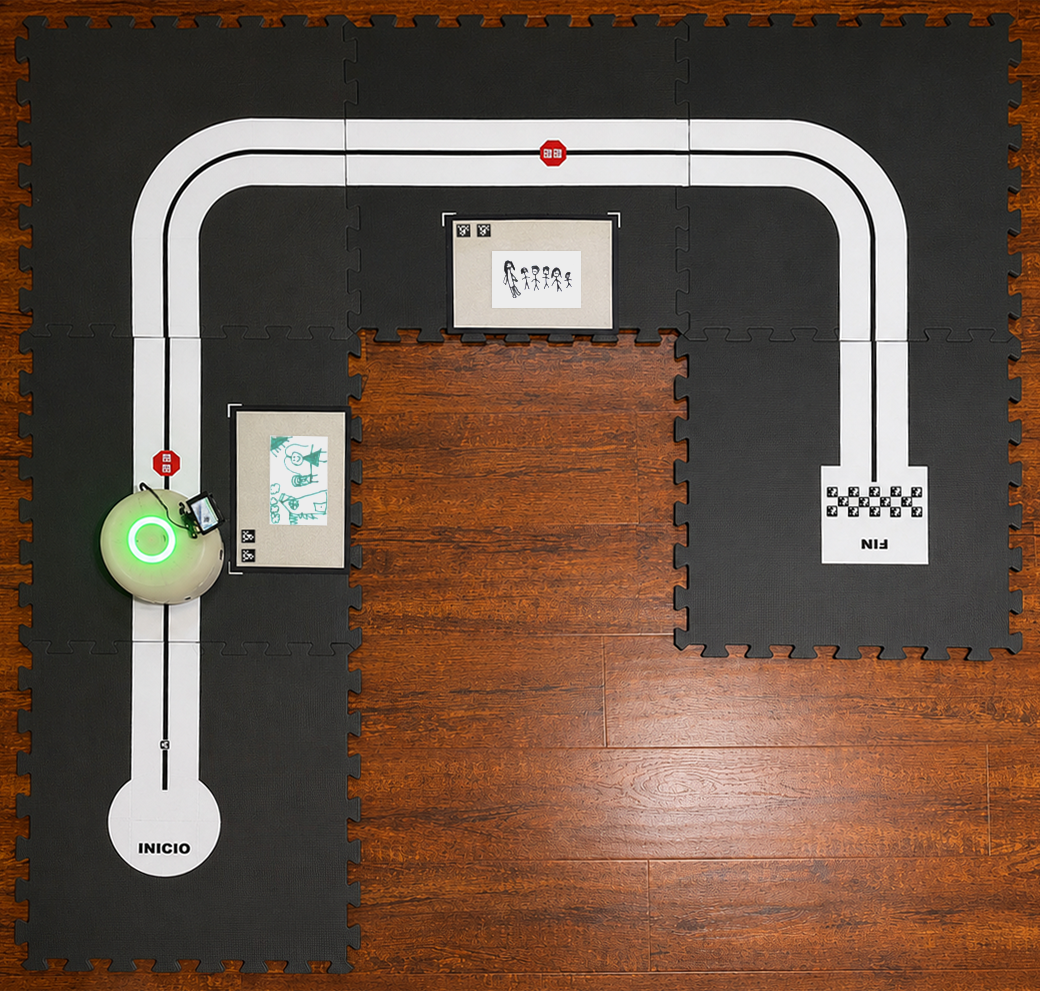
\includegraphics[width=\linewidth]{images/tablero/robotito-recorrido-foto-final.png}
    \end{subfigure}

    \caption{Montaje completo de la actividad. En la imagen se pueden observar el tablero modular, la línea que sigue Robotito durante el recorrido, el propio Robotito, los tags de referencia utilizados para detener o guiar la ejecución, las estaciones donde se ubican las tarjetas, y las tarjetas con dibujos colocadas por los estudiantes. También se observan el punto de inicio y el punto de fin del recorrido.}
    \label{fig:foto-tablero-completo}
\end{figure}

\section{Objetivos}

El objetivo general del proyecto es desarrollar una extensión de la plataforma Robotito que permita ejecutar una actividad educativa utilizando las capacidades de percepción visual brindada por la cámara HuskyLens, como seguimiento de línea y lectura de tags, además del procesamiento de los datos obtenidos por parte del robot, configuración inalámbrica desde una aplicación web y un sistema de control basado en árboles de comportamiento (\textit{Behavior Trees}). Para eso se determinaron los siguientes objetivos específicos:

\begin{itemize}
    \item Implementar la comunicación entre la cámara HuskyLens y la placa SparkFun ESP32 Thing mediante el bus I2C.
    \item Traducir y adaptar el módulo de control de la cámara al entorno Lua RTOS de Robotito.
    \item Diseñar e implementar un módulo propio de \textit{Behavior Trees}, que funcione como biblioteca de control general reutilizable para futuros proyectos.
    \item Integrar el sistema de percepción visual y el controlador BT dentro del flujo de tareas del robot.
    \item Desarrollar una actividad educativa basada en las capacidades de lectura de HuskyLens: seguimiento de línea, lectura de tags y validación de secuencias por parte del procesamiento del robot.
    \item Documentar la impresión de docentes y estudiantes sobre la actividad a partir de instancias piloto realizadas en un entorno similar al de una clase real.
    \item Extender el módulo existente de comunicación Bluetooth Low Energy (BLE) de Robotito para permitir la transferencia inalámbrica de configuraciones de actividad, con persistencia de datos en la memoria no volátil (NVS) de ESP32 Thing.
    \item Desarrollar un configurador web que permita registrar tags, definir secuencias de recorrido y enviarlas al robot sin necesidad de modificar el firmware.
\end{itemize}


Finalmente, la solución debe permitir separar con claridad la configuración de la actividad, la percepción visual y la lógica de control. Esto se ubicará en una biblioteca desarrollada que debe permitir que otros docentes e investigadores reutilicen los nodos de control en nuevos proyectos sin necesidad de modificar el código base. Cumpliendo con estos objetivos, se espera obtener una versión extendida de Robotito capaz de ejecutar una actividad configurable mediante un comportamiento autónomo organizado con árboles de comportamiento. 

\section{Organización del documento}

El presente trabajo se estructura en seis capítulos y un apéndice técnico.

En el Capítulo~\ref{cap:antecedentes} se presenta una revisión de
antecedentes centrada en la plataforma Robotito y en los robots educativos
existentes para actividades secuenciales, que sirvieron de referencia para
definir el alcance de este proyecto.

En el Capítulo~\ref{cap:analisis} se expone el análisis del problema y el
diseño de la solución. Allí se retoma el problema abordado, se detallan los
requerimientos identificados y se presenta el diseño general del sistema,
incluyendo los módulos a implementar y la actividad educativa propuesta.

En el Capítulo~\ref{cap:implementacion} se describe la implementación de la
solución, organizada en cuatro secciones. En primer lugar, se presenta el
módulo de percepción visual con HuskyLens, detallando su funcionamiento y su
integración con Robotito mediante el protocolo I2C. Luego se describe el
control del comportamiento mediante Árboles de Comportamiento (\textit{Behavior
Trees}), incluyendo sus fundamentos teóricos y la arquitectura del módulo
desarrollado. A continuación se presenta el configurador web utilizado para
la preparación de secuencias, y finalmente se detalla la configuración de
actividades y la comunicación BLE entre el configurador y el robot.

En el Capítulo~\ref{cap:experimentacion} se documenta la experimentación
realizada, tanto desde el punto de vista técnico como pedagógico:
entrevistas con docentes, sesiones prácticas con estudiantes, análisis de
resultados y ajustes realizados a partir del feedback.

En el Capítulo~\ref{cap:conclusiones} se presentan las conclusiones
generales y las líneas de trabajo futuro.

Finalmente, el apéndice reúne material complementario. 
Las referencias bibliográficas se presentan al final del documento.
\chapter{Revisión de antecedentes}
\label{cap:antecedentes}

\section{Robotito}

El robot Robotito fue desarrollado en la Facultad de Ingeniería de la Universidad de la República, pensado para introducir conceptos de robótica y pensamiento computacional en niños de entre 4 y 7 años. Se programa reorganizando los objetos de su entorno, sin necesidad de una interfaz de programación explícita. Previo a este proyecto, contaba con dos modalidades de interacción.

La primera modalidad utilizaba un sensor de color, ubicado en la base del robot, para detectar tarjetas de colores colocadas sobre la superficie de juego. Cada color indicaba una dirección de movimiento y el robot cambiaba su trayectoria al pasar sobre una tarjeta manteniendo el nuevo rumbo hasta encontrar otra. El estado activo se comunicaba mediante un anillo de LEDs RGB. El robot se activaba al apoyarlo en el piso y se detenía al levantarlo.

La segunda modalidad empleaba seis sensores de distancia distribuidos alrededor del robot para detectar objetos cercanos como conos. Robotito se desplazaba hacia el objeto más lejano detectado dentro de su alcance y si perdía de vista su objetivo realizaba un barrido de la zona para reencontrarlo o buscar uno nuevo.

\subsection{Actividades}

El equipo de Robotito documentó una serie de actividades organizadas de forma incremental en un libro destinado a docentes.

Las primeras actividades se centraban en la familiarización con el robot: conocer sus partes, aprender normas de uso y descubrir de forma exploratoria la relación entre las tarjetas de colores y el movimiento. A partir de allí, se introducían tareas de complejidad creciente, como resolver secuencias de tres pasos, planificar trayectorias evitando obstáculos representados con conos, o completar desafíos narrativos como ayudar al robot a recolectar frutas dispersas en la alfombra. Las actividades basadas en el sensor de distancia seguían una lógica similar, comenzando por la exploración libre del comportamiento del robot y avanzando hacia ejercicios de predicción, donde los niños debían anticipar hacia qué objeto se movería el robot antes de encenderlo.

% PONER IMÁGENES DE ACTIVIDADES DE ROBOTITO VIEJO.

\section{Robots educativos para actividades secuenciales}

Existen varios robots educativos comerciales para niños de nivel inicial y primeros años de primaria que, como Robotito, se programan sin una interfaz de programación explícita. Algunos de ellos sirvieron de referencia para pensar la actividad de este proyecto. Bee-Bot \cite{beebot} se controla mediante botones físicos sobre el propio robot. Estos permiten almacenar una secuencia de movimientos: avanzar, retroceder y girar. Cubetto \cite{cubetto}, en cambio, utiliza un tablero externo con bloques de colores insertables que codifican cada instrucción antes de ejecutar el recorrido, de forma similar a como Robotito se programa disponiendo tarjetas en su entorno.

Qobo \cite{qobo} es un robot con forma de caracol pensado para niños de 3 a 8 años. El robot avanza sobre un recorrido armado con tarjetas tipo puzle y un sensor ubicado en su base lee la instrucción impresa en cada una a medida que las va recorriendo.

En todos estos casos la interacción se resuelve con sensores de contacto, lectura óptica de patrones impresos o botones, sin cámara que permita al robot interpretar su entorno.

\begin{figure}[H]
    \centering
    \begin{subfigure}[b]{0.31\textwidth}
        \centering
        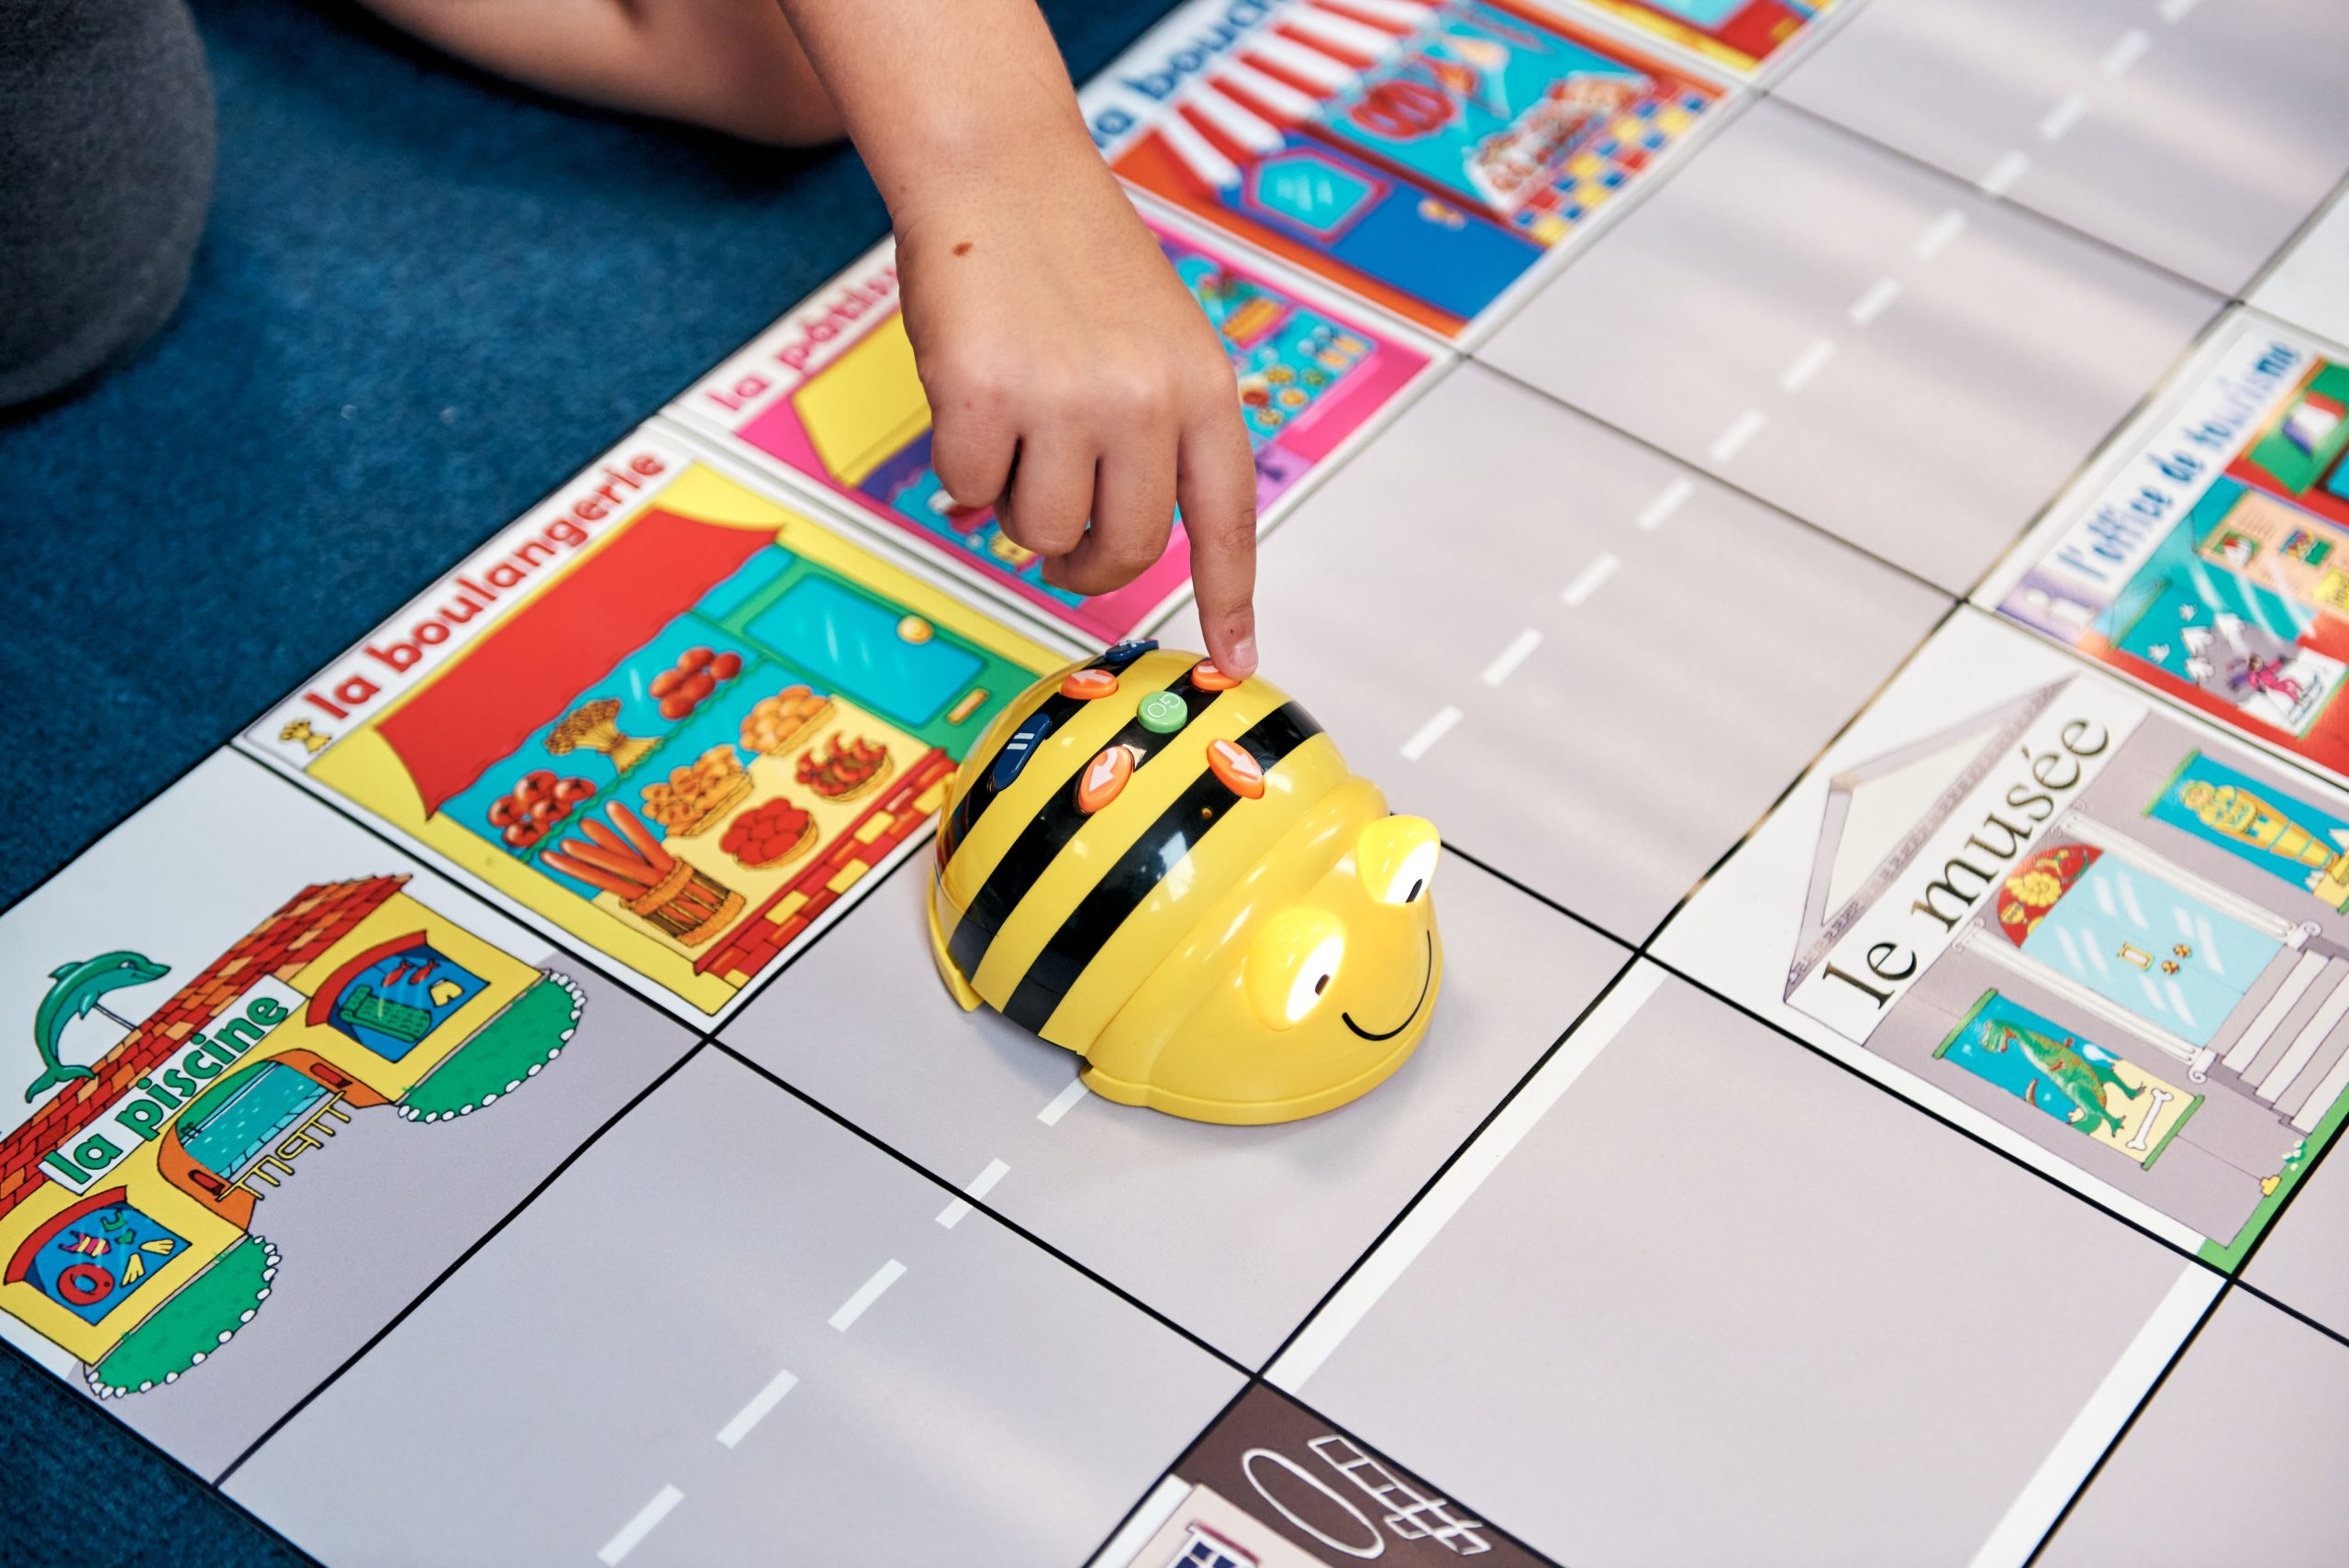
\includegraphics[height=4cm,width=\linewidth,keepaspectratio]{images/antecedentes/bee-bot.jpg}
        \caption{Bee-Bot}
    \end{subfigure}
    \hfill
    \begin{subfigure}[b]{0.31\textwidth}
        \centering
        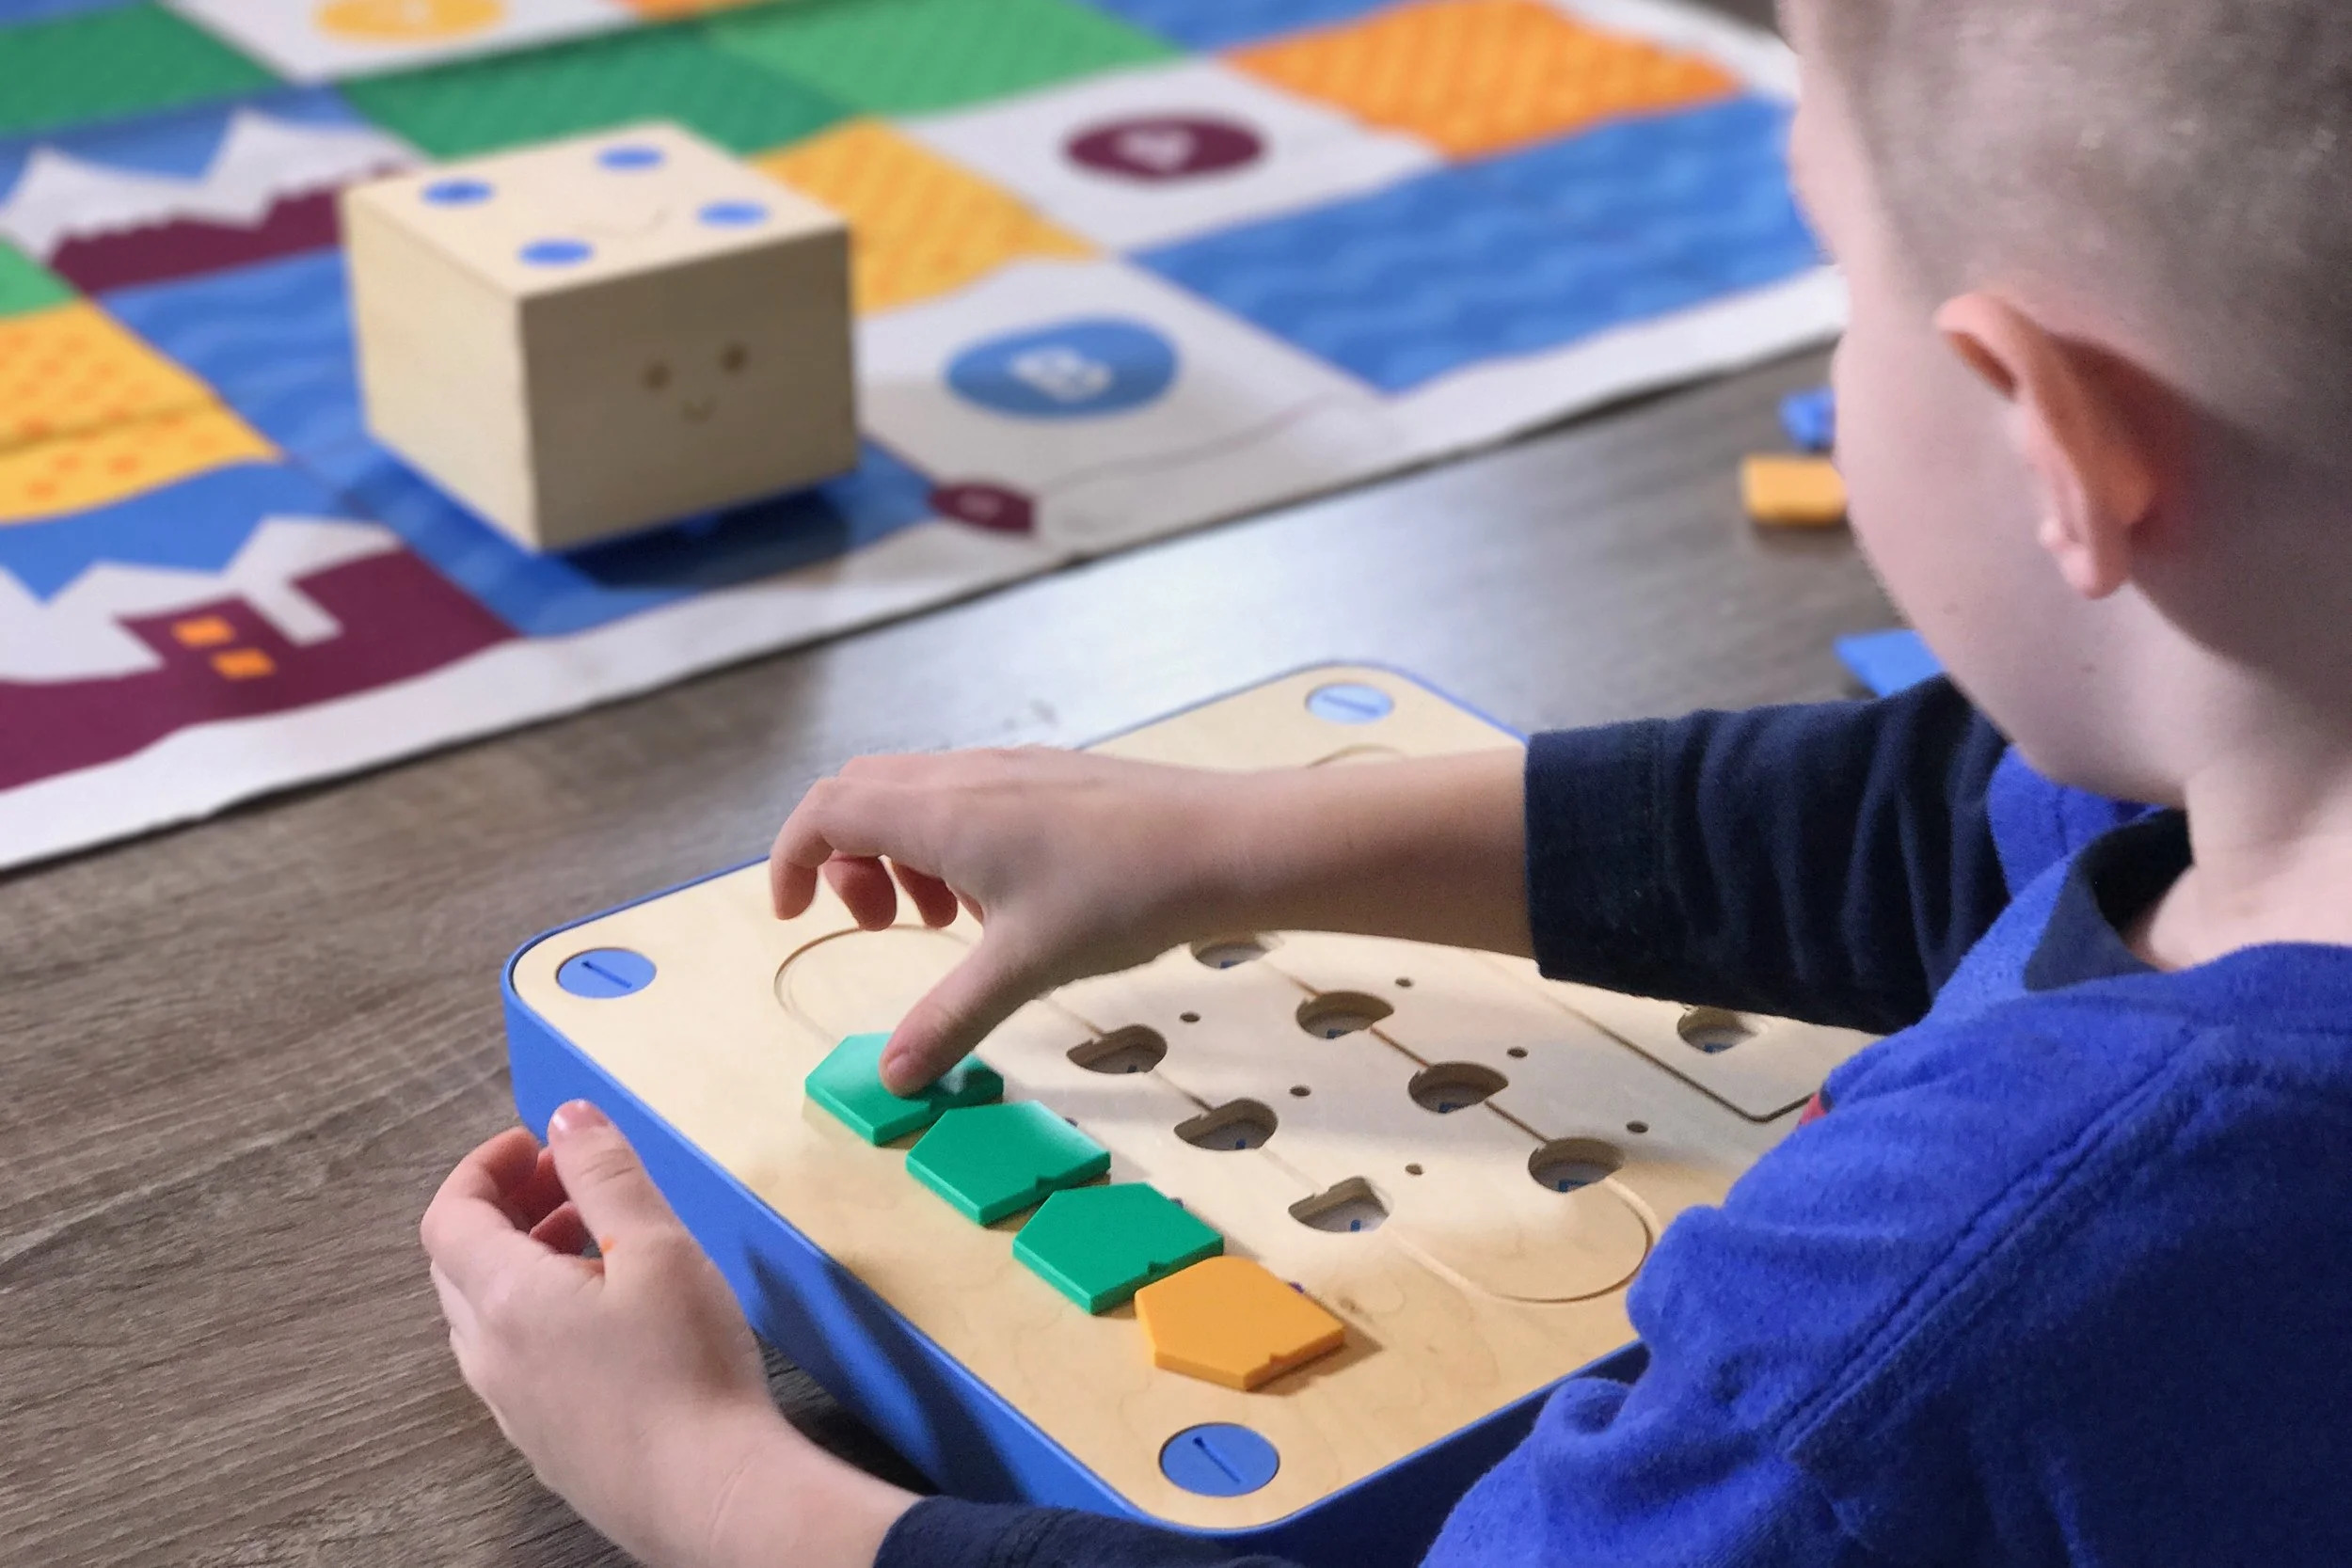
\includegraphics[height=4cm,width=\linewidth,keepaspectratio]{images/antecedentes/cubetto.jpg}
        \caption{Cubetto}
    \end{subfigure}
    \hfill
    \begin{subfigure}[b]{0.31\textwidth}
        \centering
        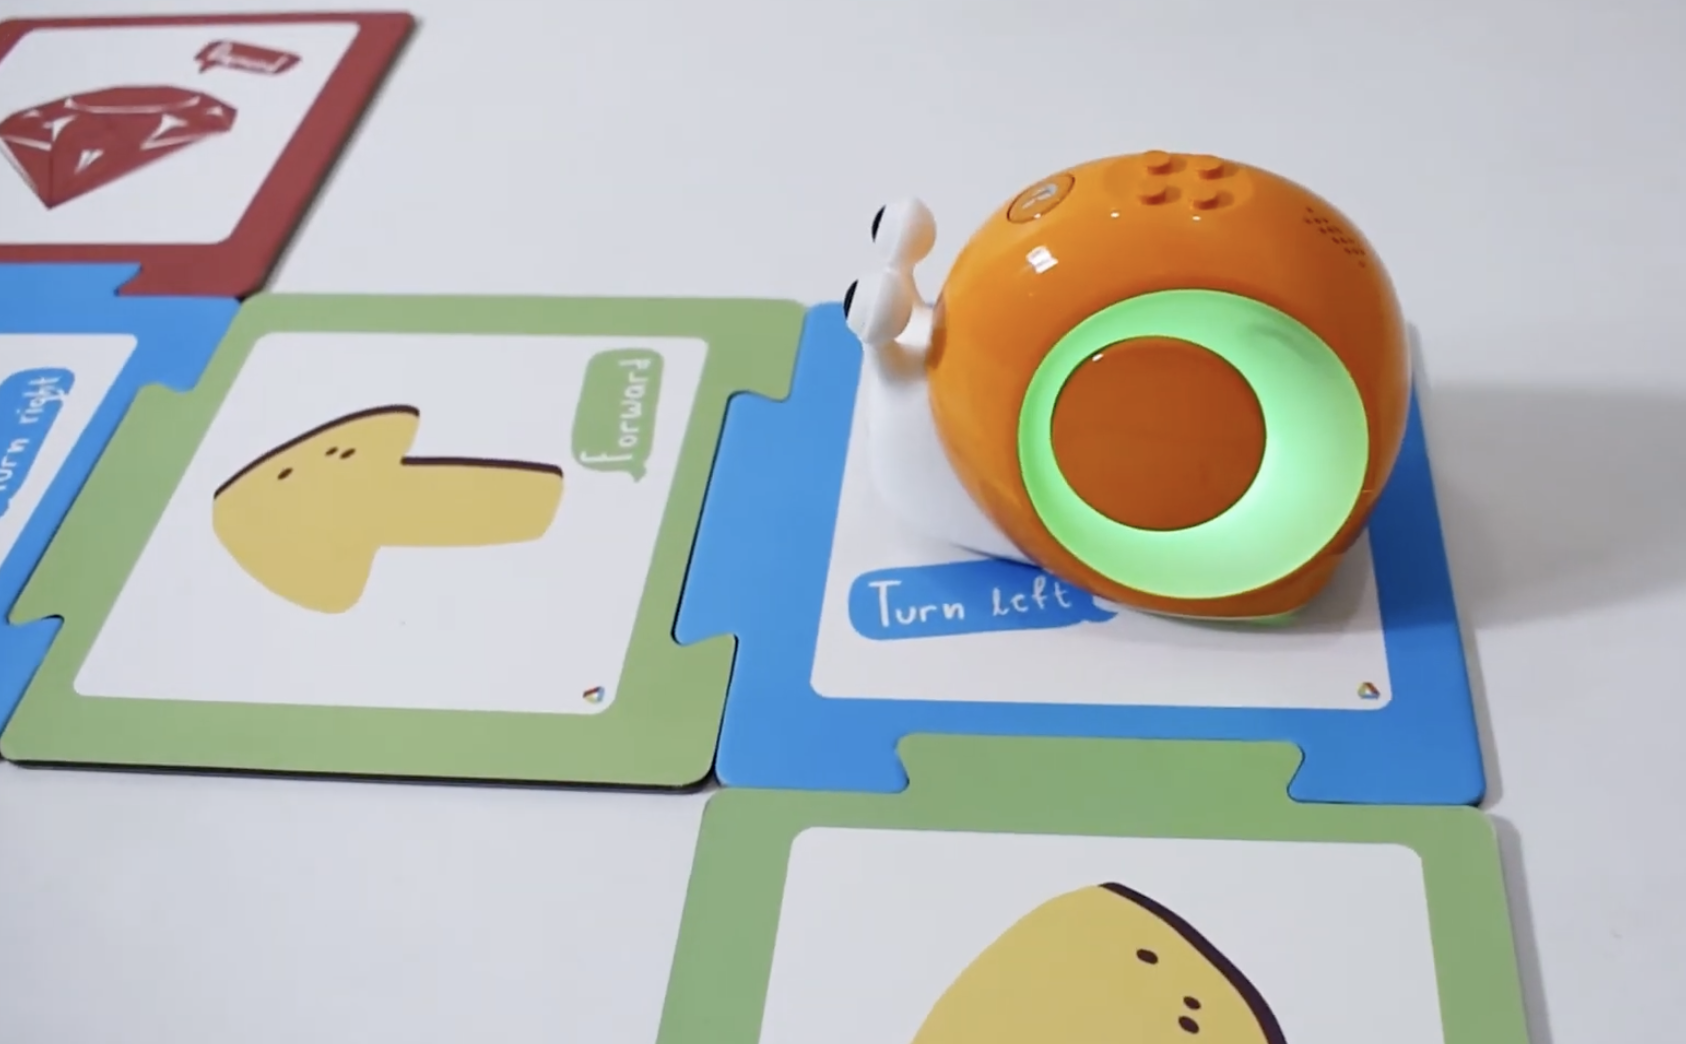
\includegraphics[height=4cm,width=\linewidth,keepaspectratio]{images/antecedentes/qobo.png}
        \caption{Qobo}
    \end{subfigure}
    \caption{Robots educativos con lógica de programación similar a Robotito.}
    \label{fig:robots-antecedentes}
\end{figure}

% ================== INICIO CAP 3 (ANALISIS & DISEÑO) ==================

\chapter{Análisis del problema y diseño de la solución}
\label{cap:analisis}

% Aclarar que parte de la premisa fue incorporar una cámara a robotito y que nuestro planteo fue cómo usarla para poder lograr dinámicas en centros educativos con niños.

% Hablar de las limitantes que tiene Robotito v1 (tuvimos que usar la cámara para cosas que pensábamos usar el sensor de rgb por ejemplo).

% Mencionar los módulos a implementar (no el cómo los implementamos) 
% - HuskyLens.
% - Behavior Tree.
% - Web
% - BLE.

% Incorporar una definición clara del alcance funcional -> Mencionar los pasos de la actividad, qué partes tiene (encastrables, tags, linea), desarrollo de la actividad. Argumentar las decisiones tomadas para la solución (tags, colores, config, pista, etc)

% Imágenes del tablero

\section{Análisis del problema}

Robotito forma parte de un proyecto de robótica educativa en constante crecimiento que ha recibido diversas modificaciones a lo largo del tiempo, con el principal objetivo de ampliar sus capacidades de programación y interacción. 

Un ejemplo es el trabajo de \citeA{hitta2022configuracionRobotito}, en el que se desarrolló una interfaz de programación visual basada en Blockly. Esta interfaz permite que usuarios sin conocimientos de programación definan nuevos comportamientos para Robotito mediante una aplicación móvil. Posteriormente, \citeA{silveira2024robotitoRFID} desarrolló una interfaz de programación basada en tarjetas con tecnología RFID. Es una propuesta interesante que permite representar físicamente instrucciones y secuencias, facilitando el trabajo de conceptos de pensamiento computacional en actividades orientadas a la educación inicial.

De manera similar, este trabajo se enfoca particularmente en el proceso de integración de una herramienta de procesamiento de imágenes a Robotito, con el objetivo de extender su capacidad de relacionarse con su entorno y de esa manera permitir el planteo de actividades más complejas con materiales variados y más atractivos en un entorno infantil. 

\subsection{Problemas identificados}

Originalmente la versión de Robotito sobre el que se trabajó contaba con un sensor en la parte inferior de su base capaz de reconocer colores y detectar cambios de distancia. Como se mencionó en el capítulo anterior, esto permitió la realización de actividades mediante la ubicación de tarjetas de colores sobre el piso, que luego eran detectadas por el robot al ubicarse este directamente arriba, para luego producir distintas reacciones en base a qué color era detectado por el sensor. 

Si bien estas condiciones son suficientes para la realización diversas actividades con distintos niveles de dificultad, se pueden identificar algunas limitantes: cada tarjeta debe contener únicamente un color (evitando errores de lectura de color incorrecto); el robot debe estar posicionado directamente arriba de la tarjeta para poder identificar el color; si bien el sensor funciona en la mayoría de los casos, diferencias de iluminación en el entorno pueden generar inconsistencias de lectura.

Desde el punto de vista técnico, incorporar visión artificial en una plataforma embebida puede comprometer la estabilidad del sistema y afectar la capacidad de respuesta del robot. El procesamiento de imágenes requiere recursos significativos de CPU, memoria y tiempo de ejecución. En el caso de Robotito, el microcontrolador principal debe encargarse simultáneamente del control de motores, la lectura de sensores, la comunicación con otros módulos y la ejecución del entorno Lua RTOS. Además la solución a implementar debe ser estructurada de una manera que sea fácil de entender y mantener, con posibilidades de extender su funcionalidad a futuro.

\subsection{Requerimientos de la solución}

A partir de los problemas identificados se proponen siguientes requerimientos:

\begin{itemize}
    \item \textbf{Bajo impacto computacional sobre el ESP32:} el procesamiento de imágenes no debe ejecutarse directamente en el microcontrolador principal. El sistema debe recibir información visual ya procesada, en forma de datos de alto nivel utilizables por la lógica de control.

    \item \textbf{Compatibilidad con la plataforma existente:} la solución debe integrarse con la arquitectura actual de Robotito, manteniendo el uso de la placa SparkFun ESP32 Thing, Lua RTOS y los mecanismos de comunicación disponibles.

    \item \textbf{Modularidad del software:} la percepción visual, la toma de decisiones y la ejecución de acciones deben mantenerse desacopladas, de forma de facilitar el mantenimiento, la extensión y la reutilización del sistema.

    \item \textbf{Reactividad ante eventos del entorno:} el robot debe ser capaz de responder a estímulos visuales durante la ejecución de una actividad, sin depender exclusivamente de secuencias rígidas de comandos.

    \item \textbf{Integración física robusta:} la incorporación de nuevos componentes no debe afectar negativamente la estabilidad, ergonomía ni facilidad de uso del robot. La cámara debe ubicarse en una posición adecuada para la detección visual y su montaje debía ser seguro y replicable.

    \item \textbf{Aplicabilidad pedagógica:} la solución debe habilitar actividades comprensibles y manipulables por docentes y estudiantes, utilizando elementos más atractivos como parte activa de la experiencia educativa.
\end{itemize}

\section{Diseño de la solución}

Para cumplir con los requerimientos planteados se propone extender Robotito mediante una cámara HuskyLens, capaz de procesar imágenes y devolver información de alto nivel sobre los elementos detectados. De esta manera, el procesamiento visual no se realiza en el ESP32 y el robot puede reconocer elementos ubicados dentro del campo de visión de la cámara, sin depender únicamente del sensor situado en la parte inferior de su base.

La solución se organiza en módulos específicos que separan la percepción visual, el control del comportamiento y la configuración de la actividad. Esta organización permite integrar las nuevas capacidades con la arquitectura existente de Robotito, facilitar su mantenimiento y habilitar una actividad educativa configurable. A continuación se presentan los módulos necesarios para implementar la solución.

\subsection{Módulos a implementar}

La solución se organiza en cuatro módulos principales, cuyas responsabilidades se presentan a continuación. La implementación de cada uno se describe en detalle en el Capítulo 4.

En primer lugar, es necesario un módulo especializado que permita el intercambio de información entre HuskyLens y el robot. Este debe ser capaz de iniciar la comunicación con la cámara, construir mensajes y enviarlos, interpretar y validar sus respuestas, además de exponer los métodos necesarios que luego serán invocados desde el entorno de Lua RTOS.

Por otro lado, es necesario definir una capa de control organizada mediante el modelo de Árboles de Comportamiento, en la que cada nodo represente una acción, una condición o una estructura de control específica. Esta organización permite dividir el comportamiento general del robot en componentes simples y reutilizables, facilitando la incorporación de nuevas funcionalidades sin modificar por completo la lógica existente.

Finalmente, con el objetivo de facilitar la interacción del docente con Robotito y posibilitar la customización de la actividad a ser planteada, se decide implementar un configurador web en el que el usuario es capaz de editar la secuencia correcta esperada por el robot y enviársela utilizando el protocolo de comunicación BLE (Bluetooth Low Energy). Del lado del robot, es necesaria la implementación de un módulo capaz de realizar la conexión con el configurador web y transportar datos entre ambas partes, además de guardar correctamente los datos recibidos en el almacenamiento NVS (Non-Volatile Storage) de ESP32.

\section{Diseño de la actividad}

Una vez definidos los módulos a implementar se plantearon diversas actividades posibles, aplicables en entornos de educación inicial y acordes a la arquitectura actual de Robotito y las capacidades de percepción de HuskyLens. Luego de establecer ciertos requisitos y realizar algunas pruebas, se logra definir un modelo de actividad.

Una de las principales premisas establecidas es la de que el robot debe poder obtener información visual de su entorno y trasladarse según los elementos que haya identificado en cada lectura. Luego de realizar distintas pruebas con la cámara ya integrada al robot se determina que utilizar la función de Seguimiento de líneas (\textit{Line Tracking}) es una manera confiable de cumplir con este requisito. Esto trae la necesidad de encontrar una forma de detener y reanudar el recorrido en determinados momentos específicos de la actividad. Entre las funciones disponibles de HuskyLens para cumplir con este requerimiento, se observa que los modos de Reconocimiento de color (\textit{Color recognition}) y Reconocimiento de marcadores visuales (\textit{Tag recognition}) son los que presentan mejores resultados prácticos. Si bien el modo de Reconocimiento de color puede resultar útil en algunas situaciones, se descarta esta opción al encontrar ciertas inconsistencias de lectura en casos de prueba con iluminación no favorable, en los que la cámara parece no detectar un color previamente identificado en otro caso con iluminación distinta del ambiente. Por esta razón, se concluye que la actividad debe contar con diversos marcadores visuales (de tipo \textit{AprilTag}) a lo largo de un recorrido definido por una línea.

\subsection{Caso de uso}

Se propone una actividad cuyo principal objetivo es generar una instancia donde el docente presenta el concepto de secuencia ordenada utilizando a Robotito como verificador de secuencias, acercando al alumno a conceptos de robótica y pensamiento computacional. Para esto se define un sistema que consiste en tres elementos principales (además de otros que se mencionan más adelante):

\begin{itemize}
    \item Robotito con cámara HuskyLens integrada que recibe información visual del exterior y reacciona en base a los datos obtenidos.
\end{itemize}

\begin{itemize}
    \item Un tablero que contiene un recorrido (definido por una línea contínua) y varios ``puntos de parada'' (la cantidad que sea necesaria, según la cantidad de elementos de la secuencia definida por el docente) que corresponden a cada posición de la secuencia a verificar por Robotito. Cada punto de parada se determina con un tag específico a lo largo del recorrido junto a una zona específica para ubicar las tarjetas. Además, el tablero contiene un punto de partida y uno de fin, donde Robotito debe empezar y terminar el recorrido, respectivamente.
\end{itemize}

\begin{figure}[htbp]
    \centering

    % Primera fila
    \begin{subfigure}{0.25\textwidth}
        \centering
        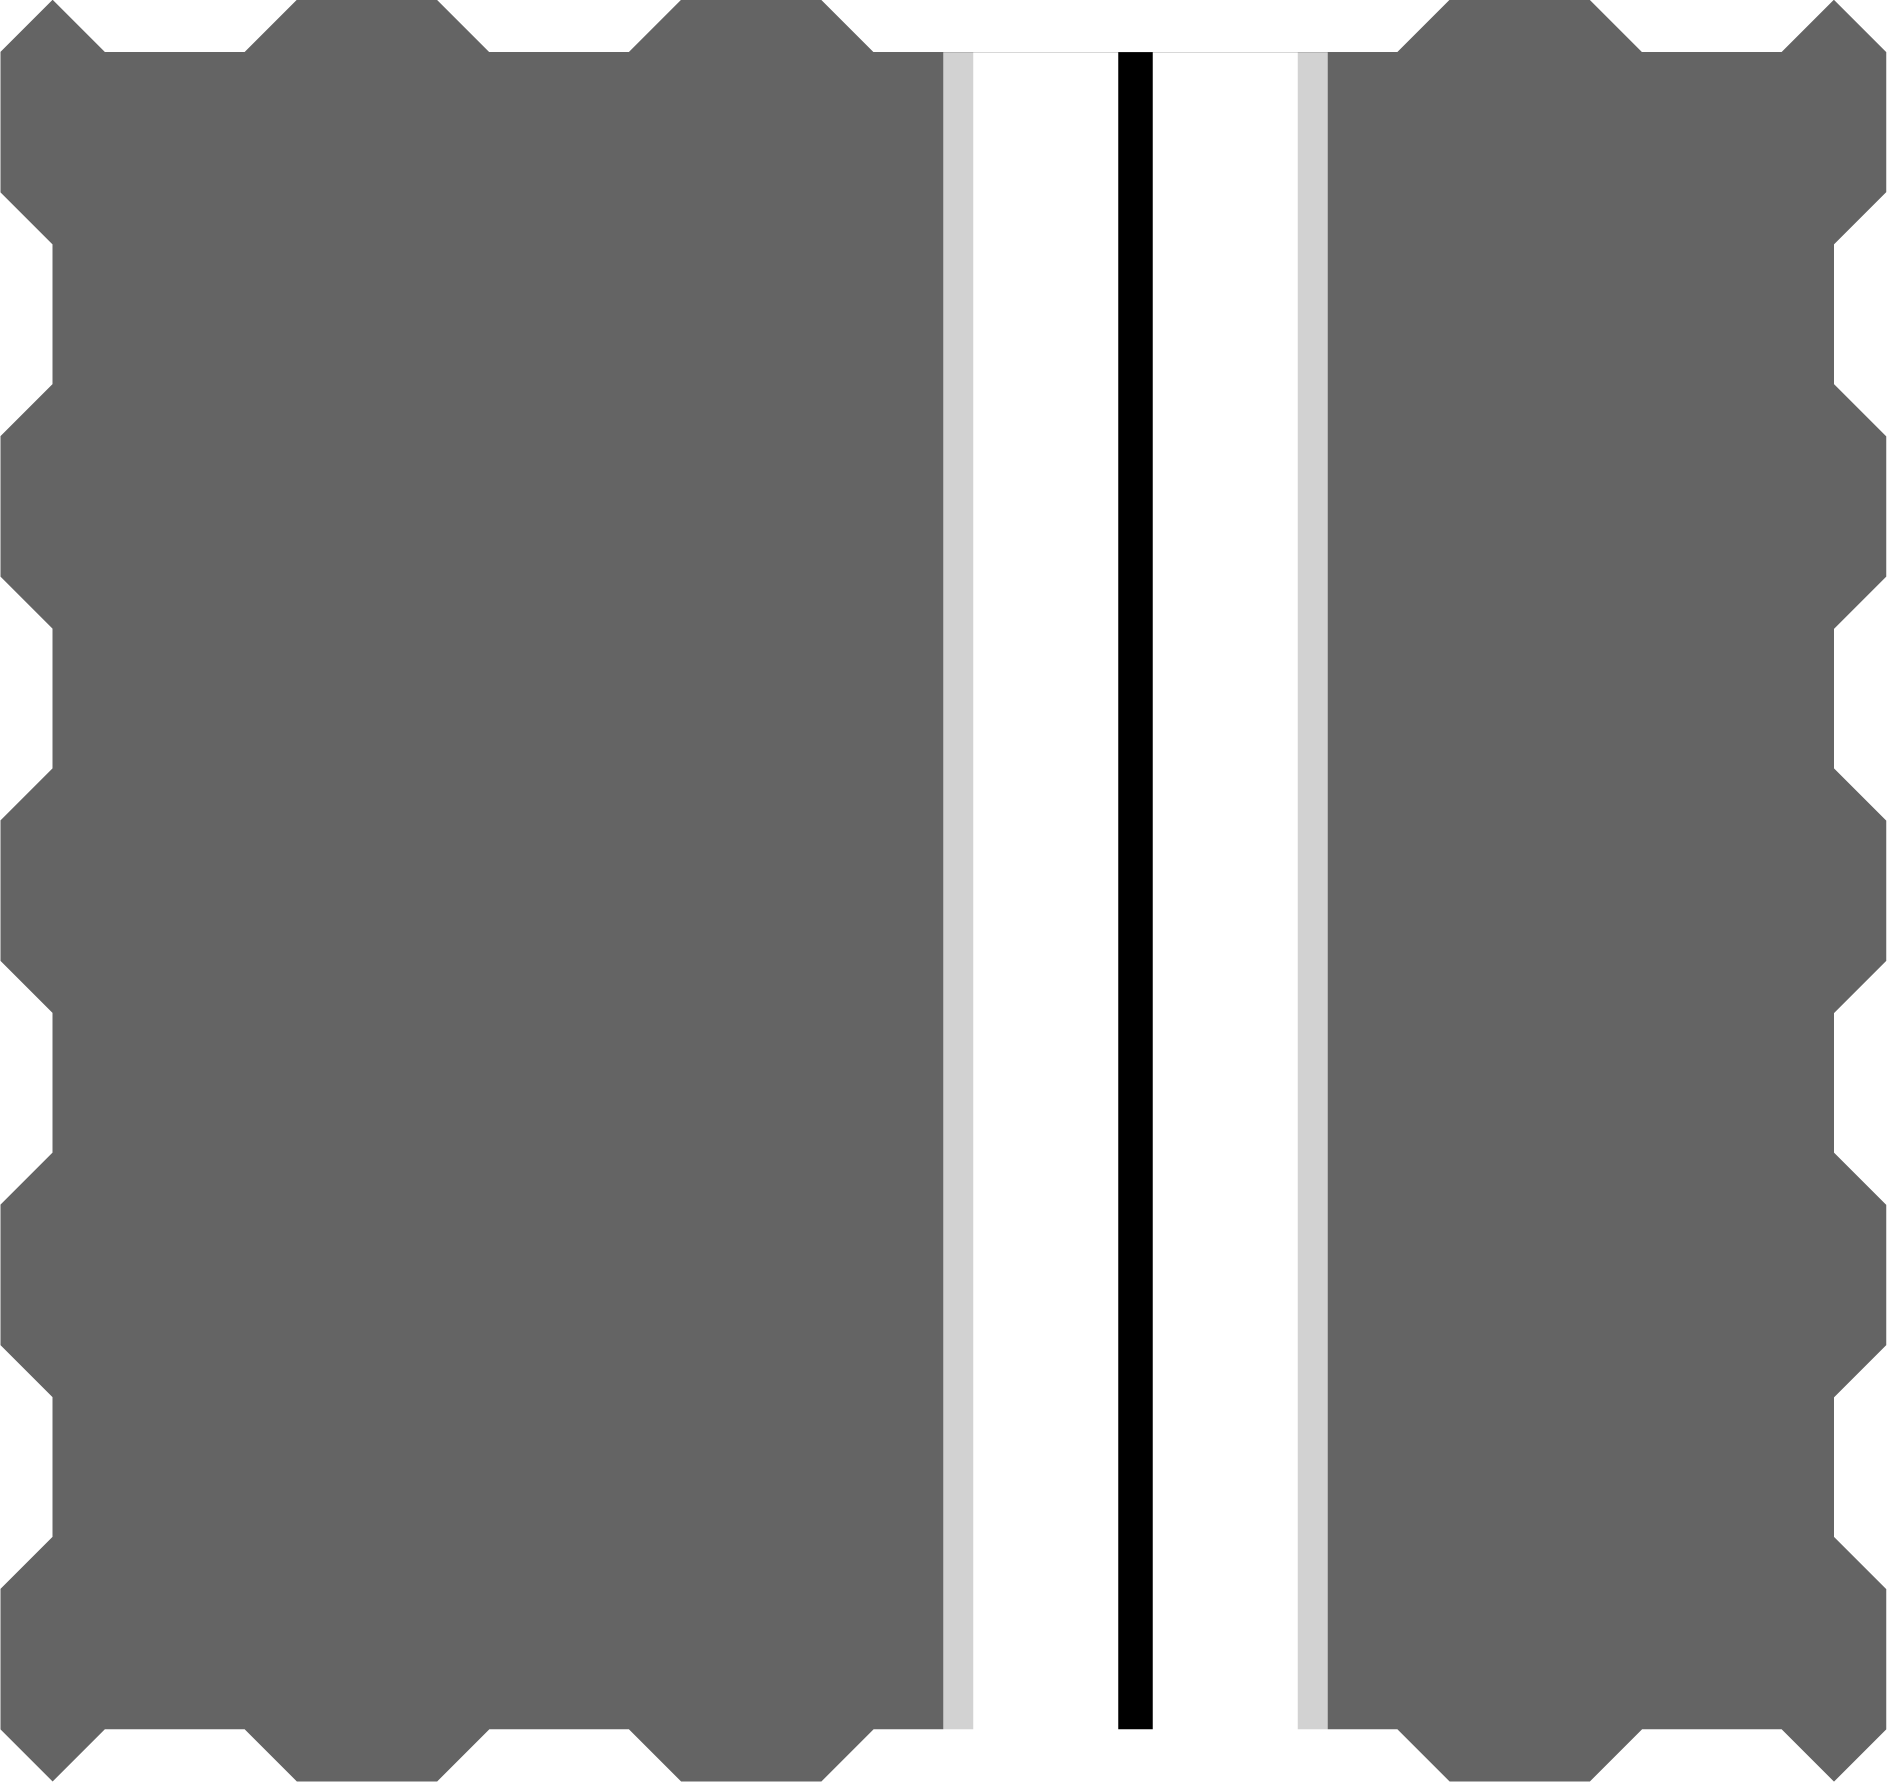
\includegraphics[width=\linewidth, angle=180]{images/tablero/tablero-recta.png}
        \caption{Pieza del tablero con recta}
    \end{subfigure}
    \hfill
    \begin{subfigure}{0.25\textwidth}
        \centering
        
\includegraphics[width=\linewidth, angle=180]{images/tablero/tablero-curva-corta.png}
        \caption{Pieza del tablero con curva corta}
    \end{subfigure}
    \hfill
    \begin{subfigure}{0.25\textwidth}
        \centering
        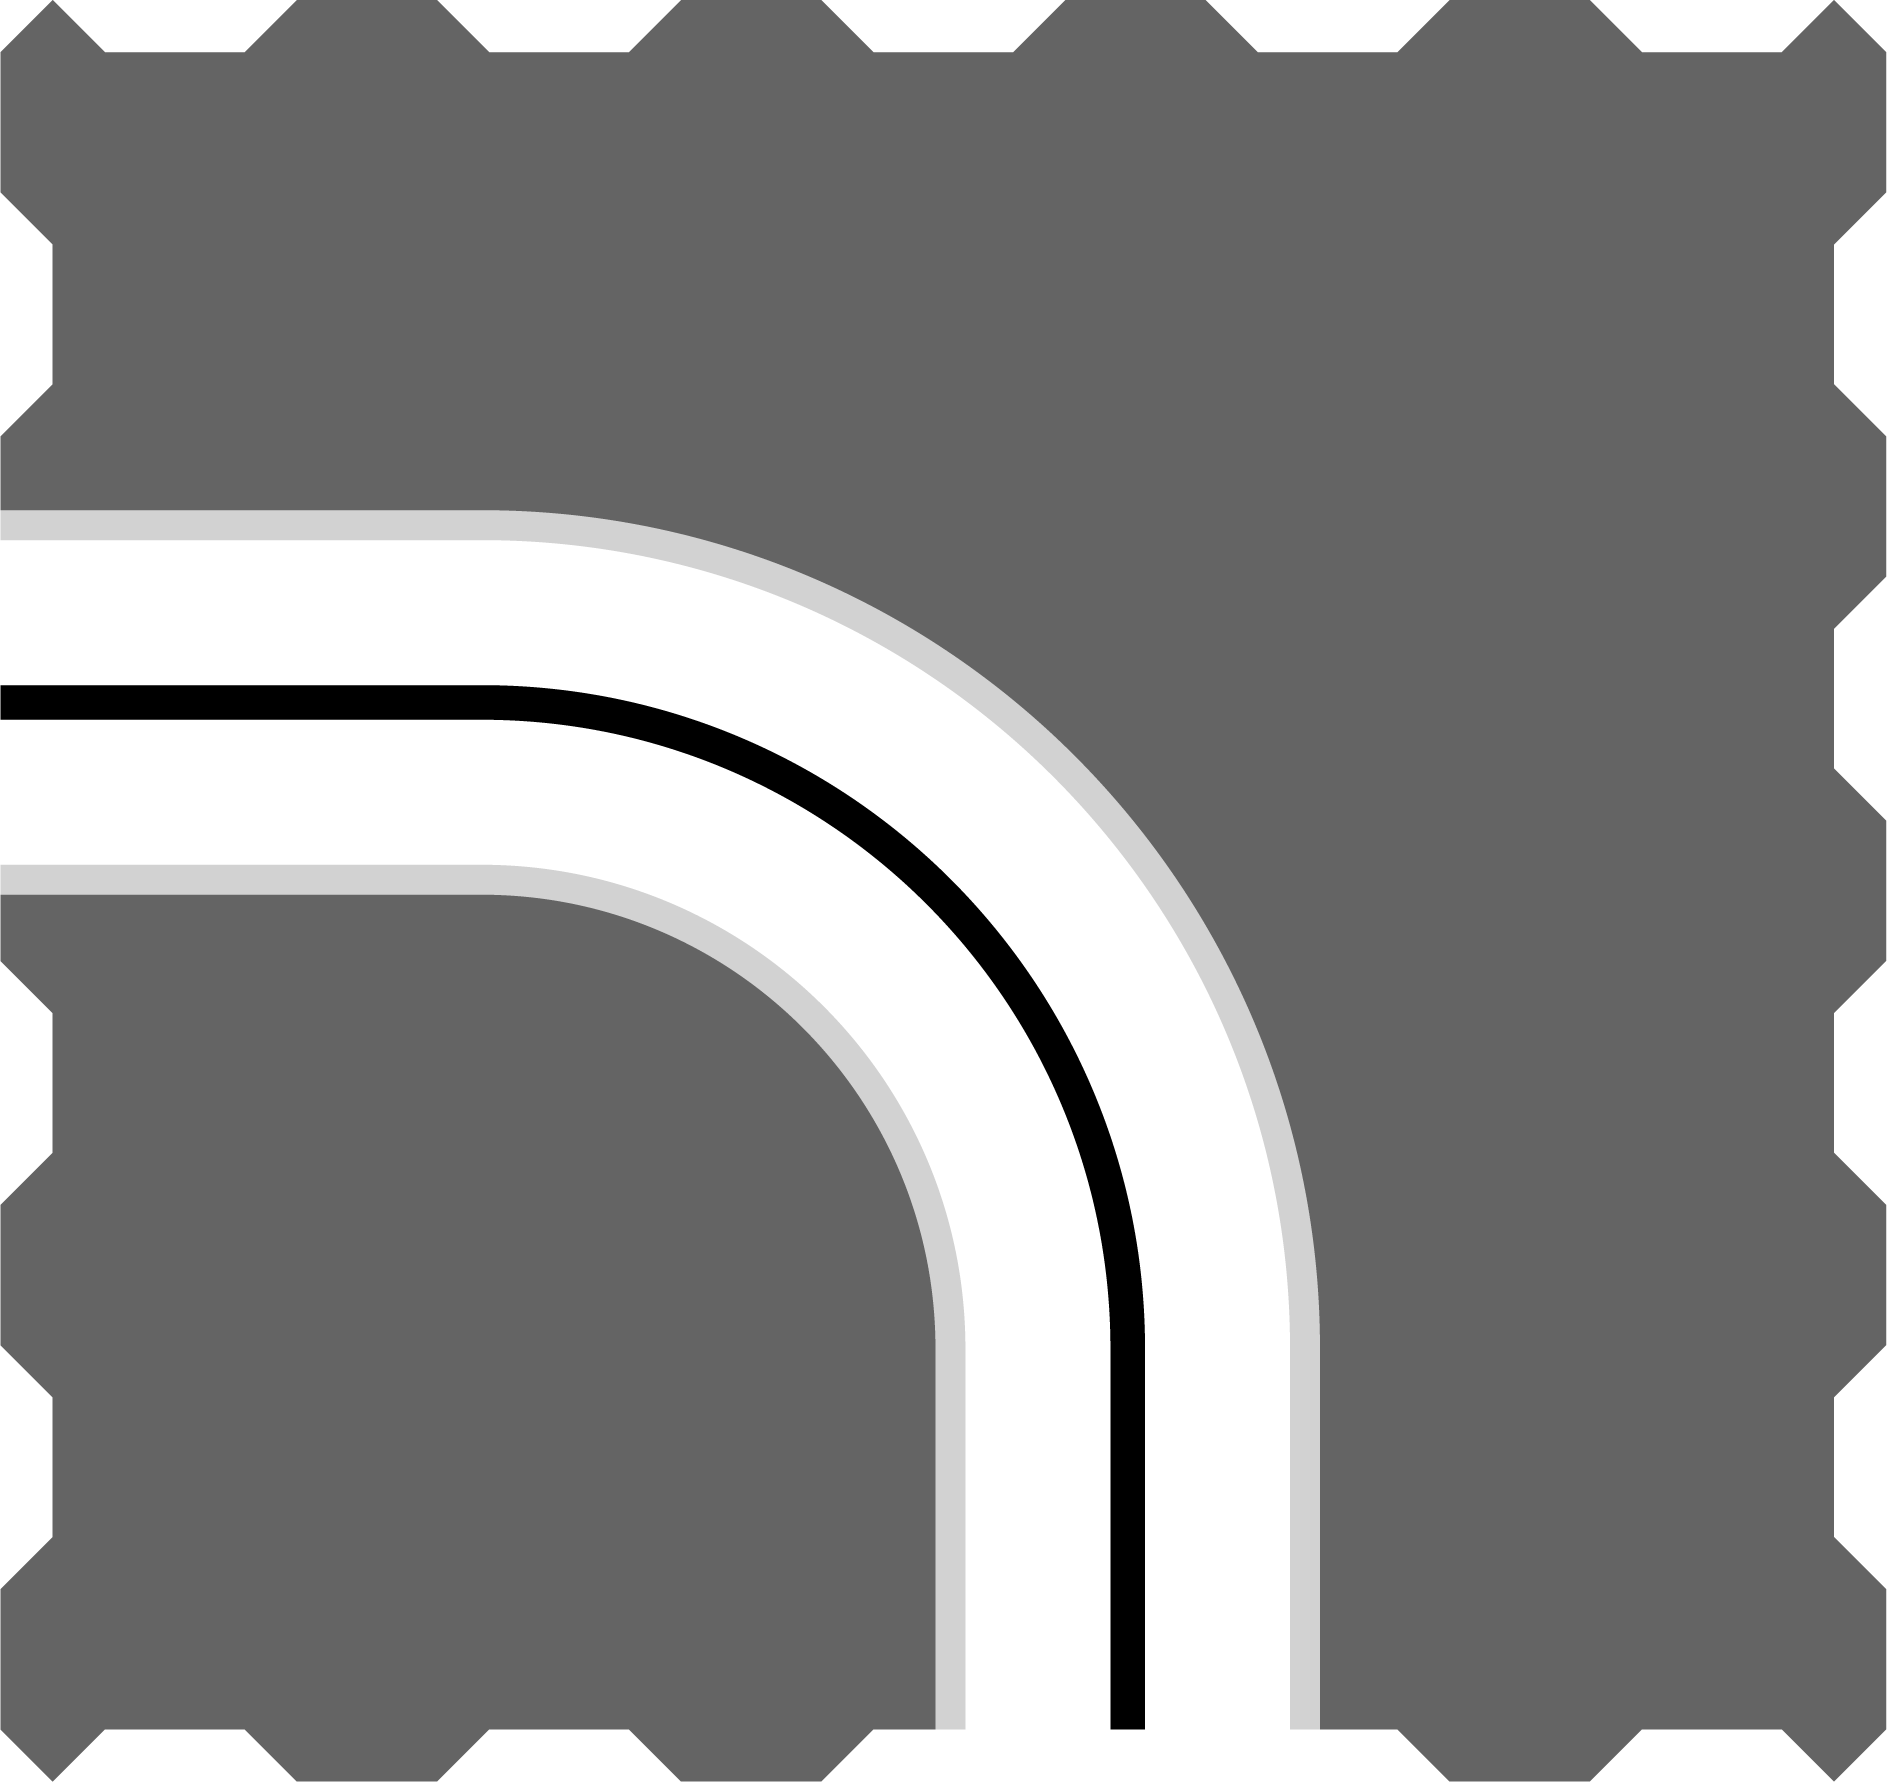
\includegraphics[width=\linewidth]{images/tablero/tablero-curva-larga.png}
        \caption{Pieza del tablero con curva larga}
    \end{subfigure}

    \vspace{0.2cm}

    % Segunda fila
    \begin{subfigure}{0.25\textwidth}
        \centering
        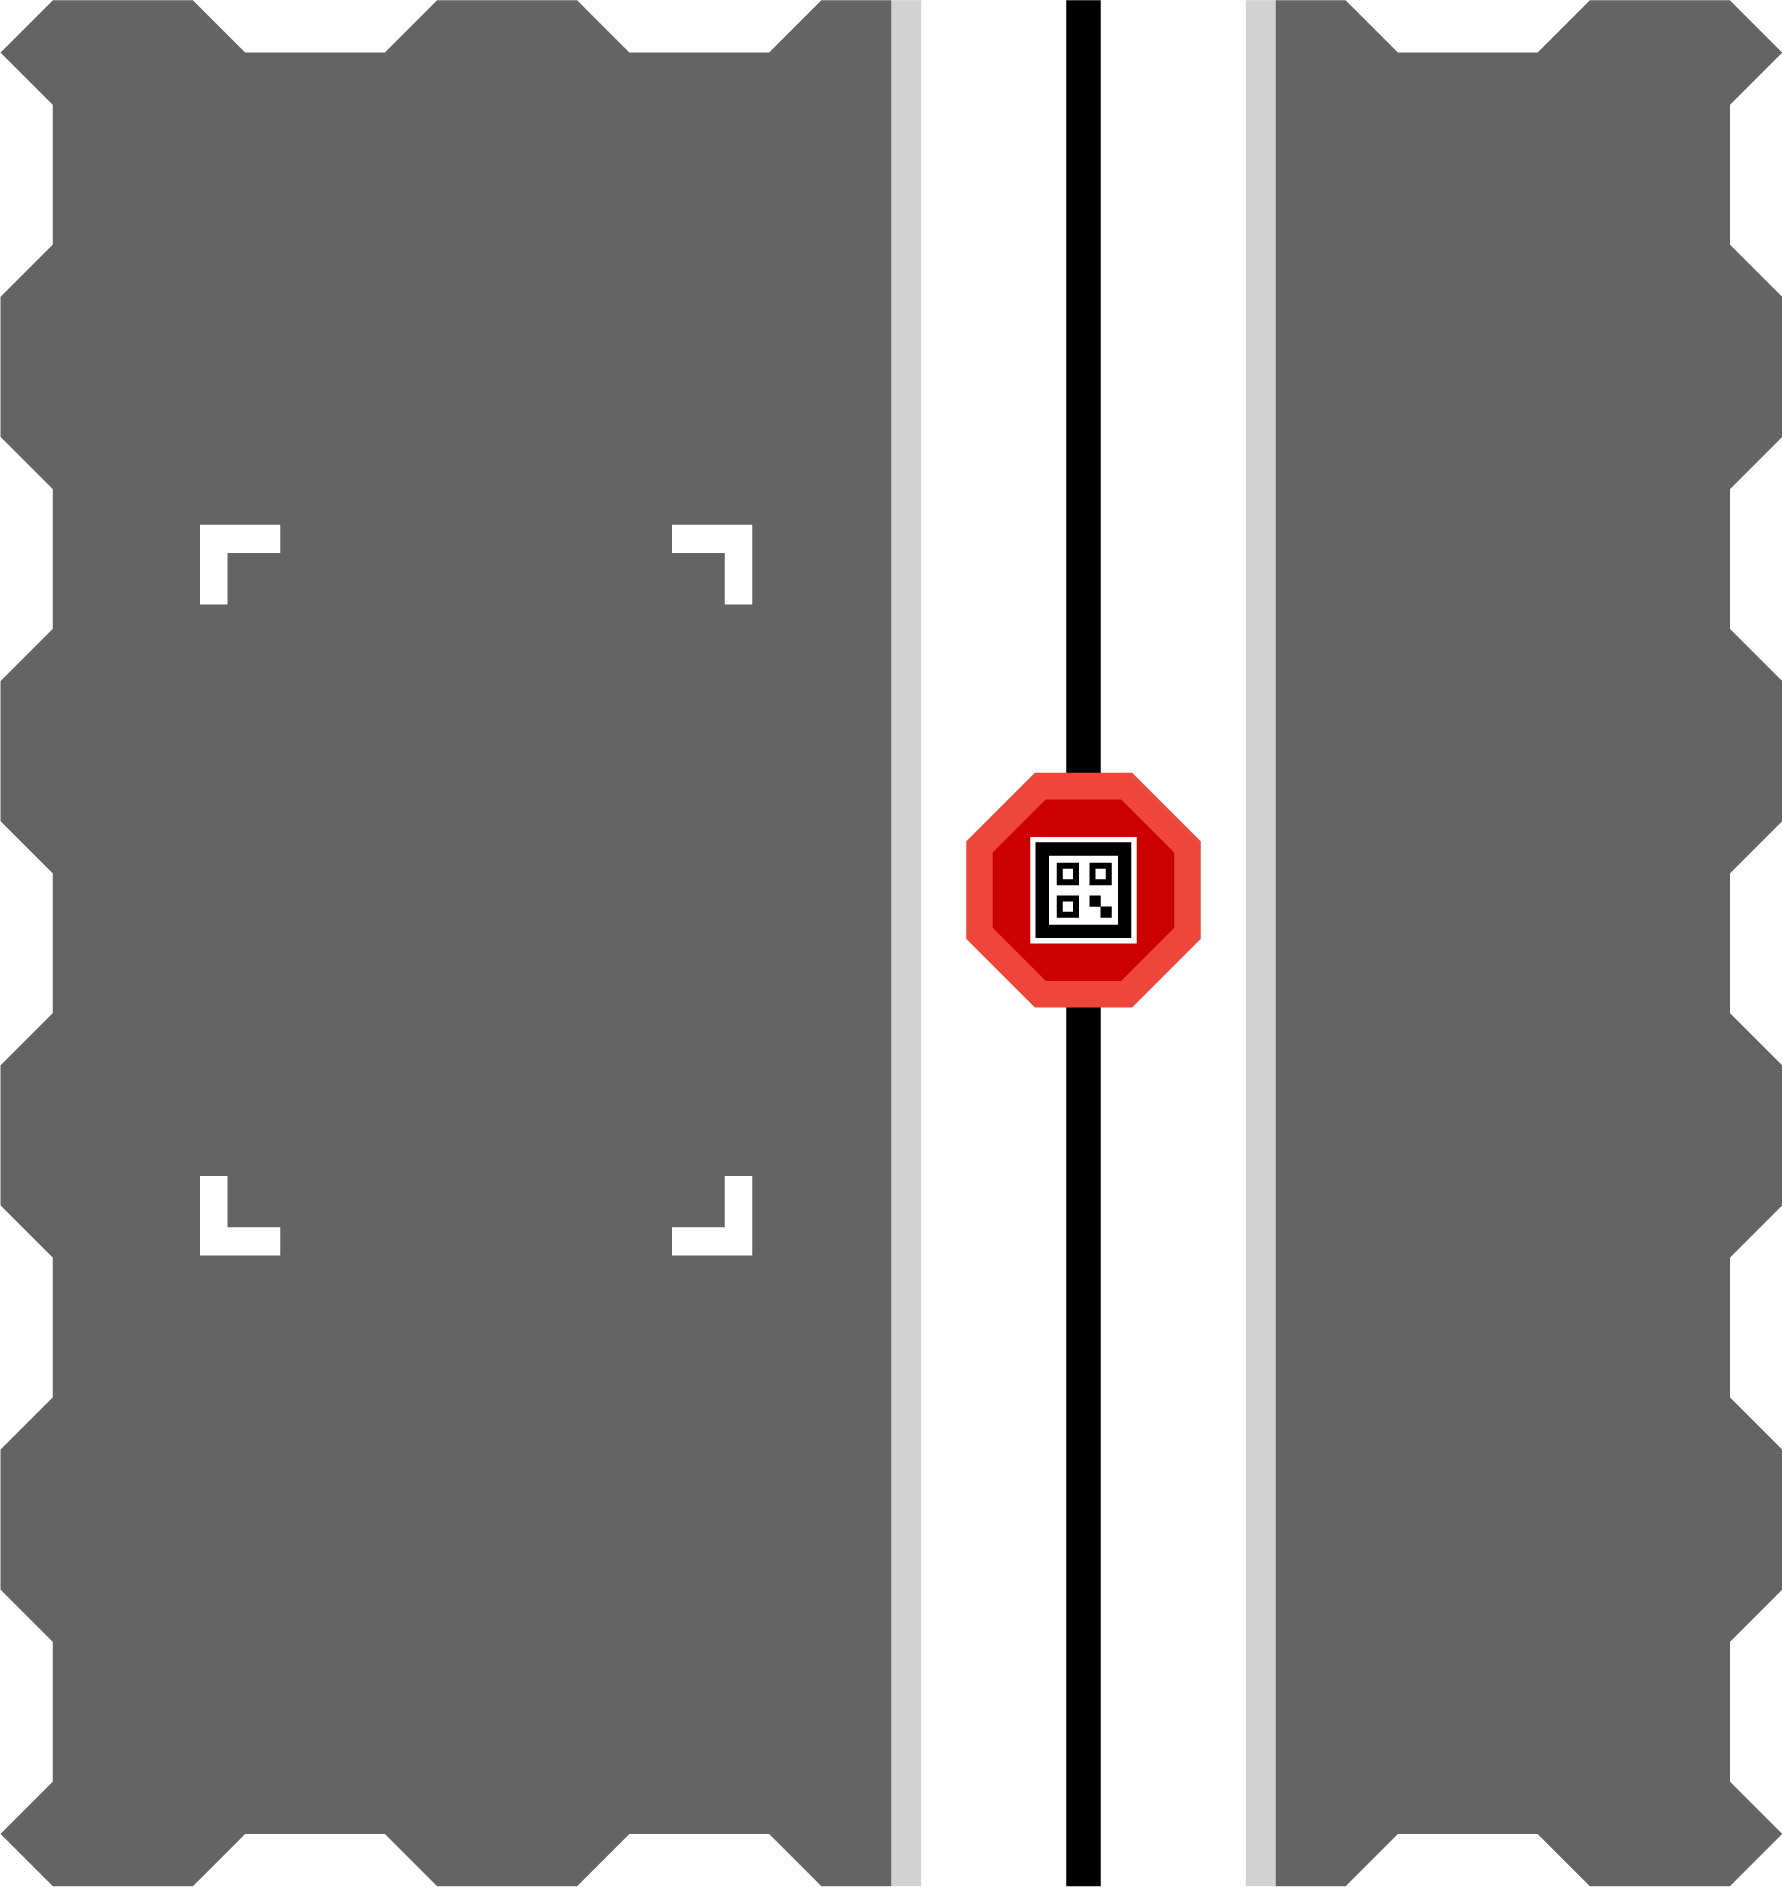
\includegraphics[width=\linewidth]{images/tablero/tablero-recta-QR.png}
        \caption{Pieza del tablero con punto de parada}
    \end{subfigure}
    \hfill
    \begin{subfigure}{0.25\textwidth}
        \centering
        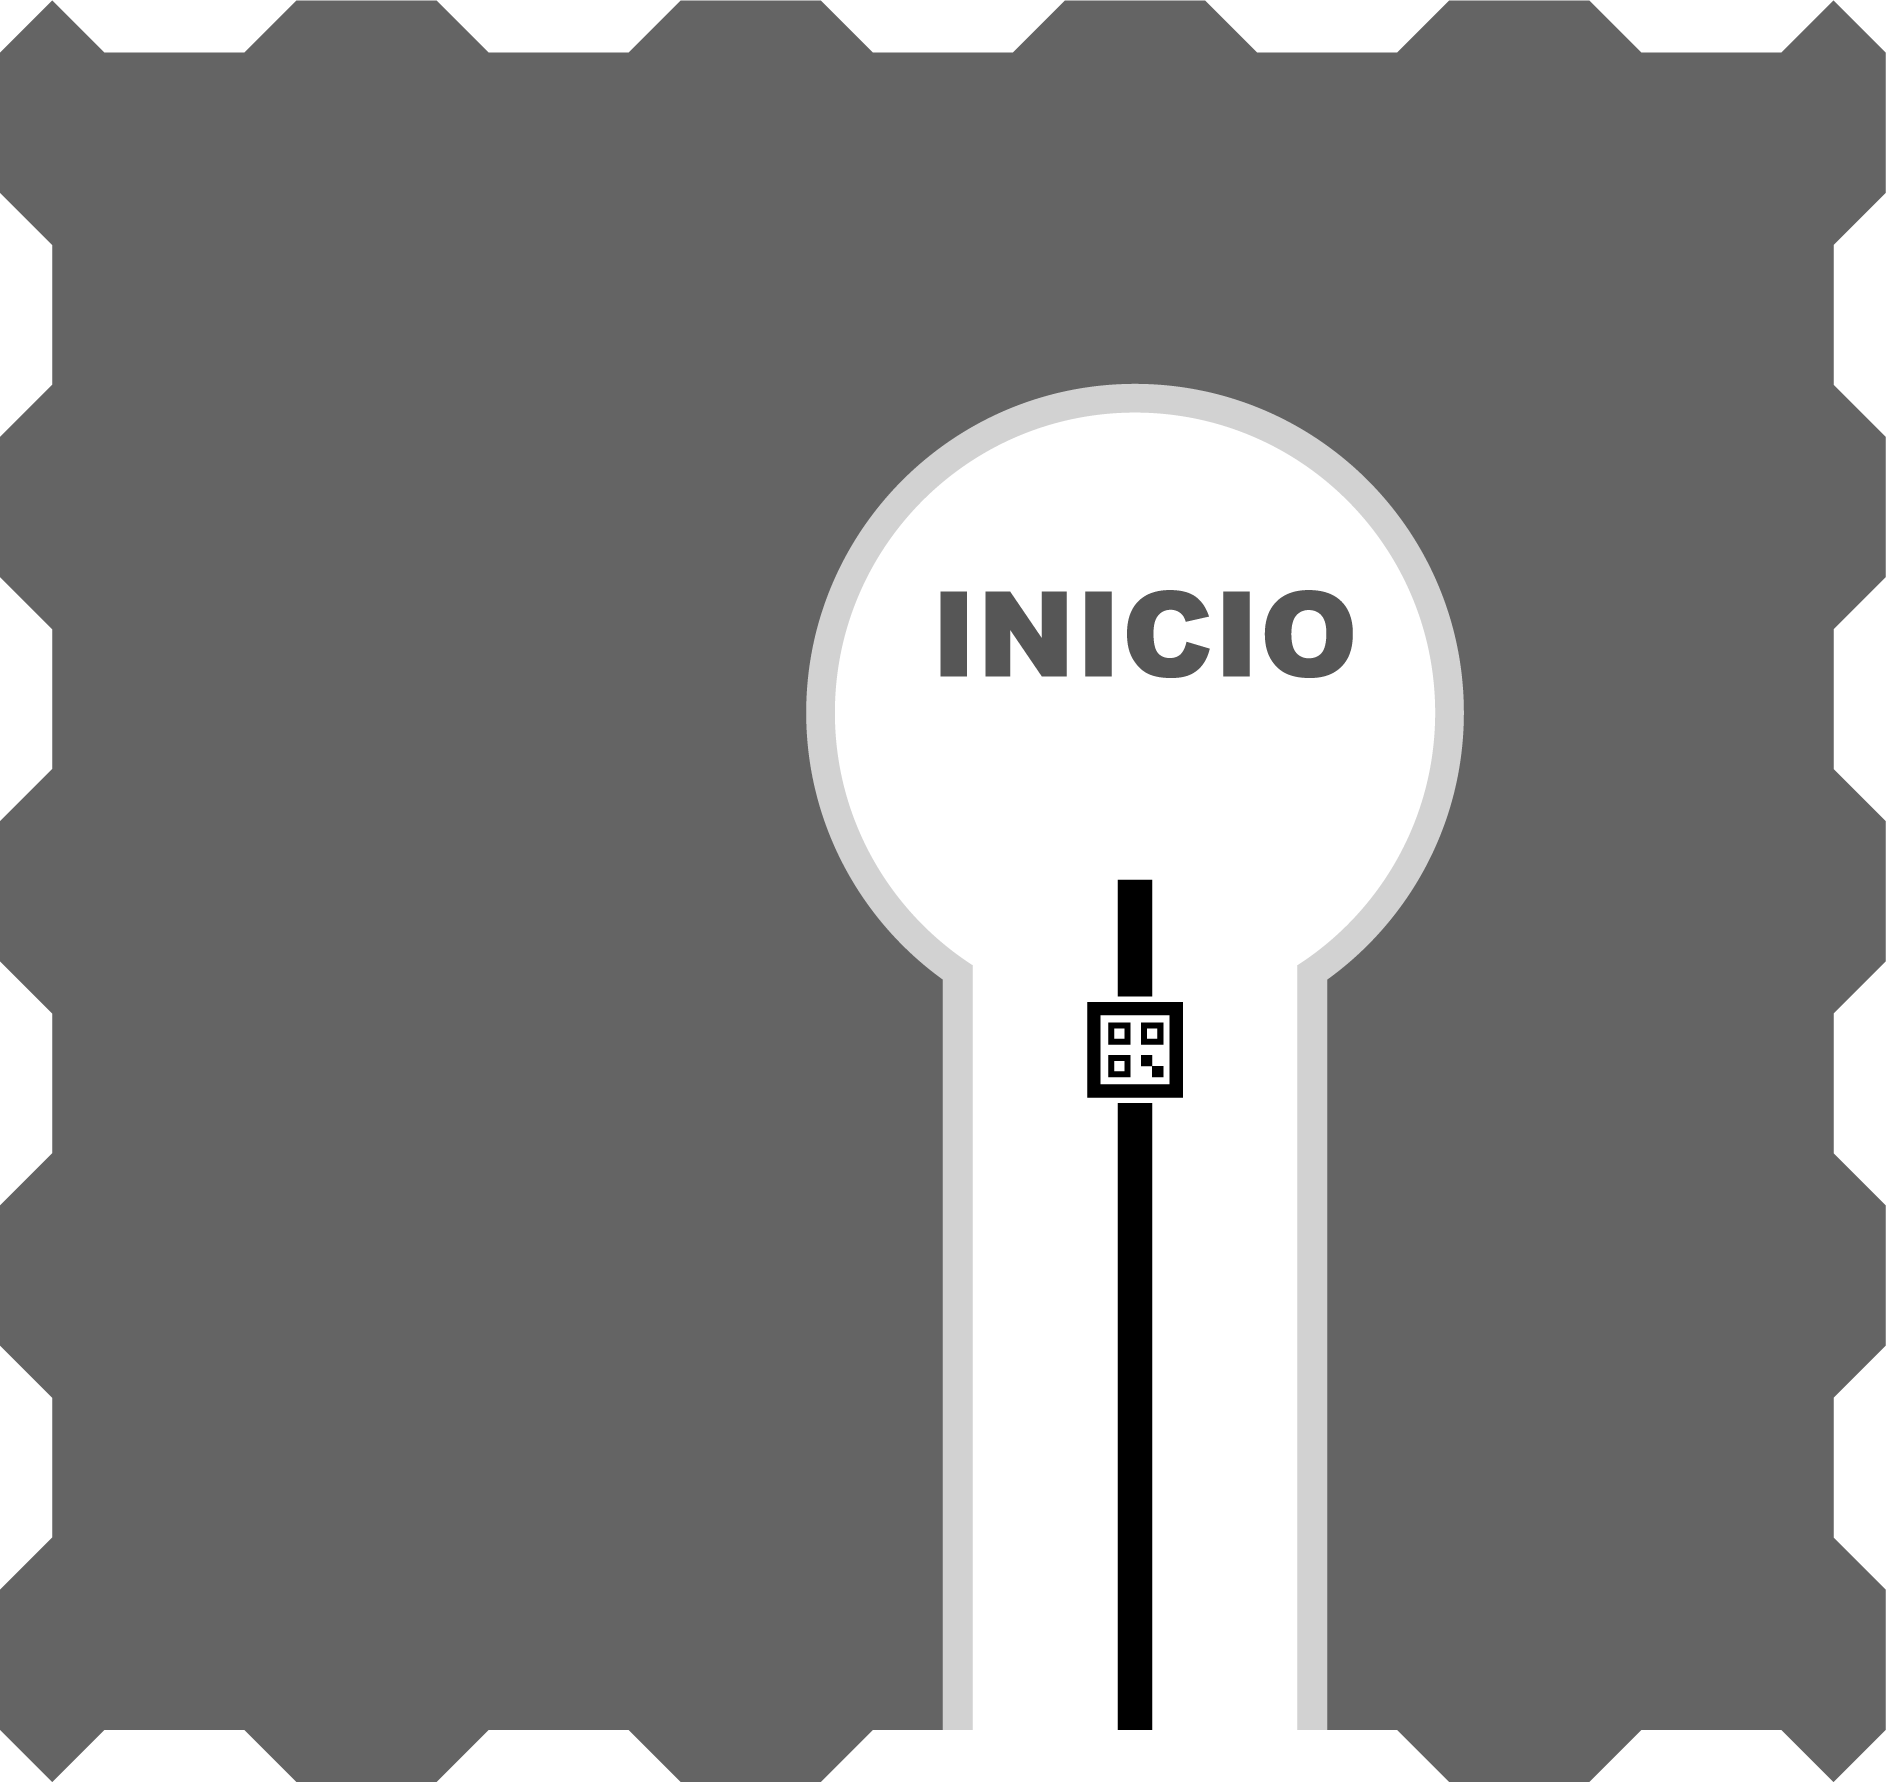
\includegraphics[width=\linewidth]{images/tablero/tablero-start.png}
        \caption{Pieza del tablero con curva corta}
    \end{subfigure}
    \hfill
    \begin{subfigure}{0.25\textwidth}
        \centering
        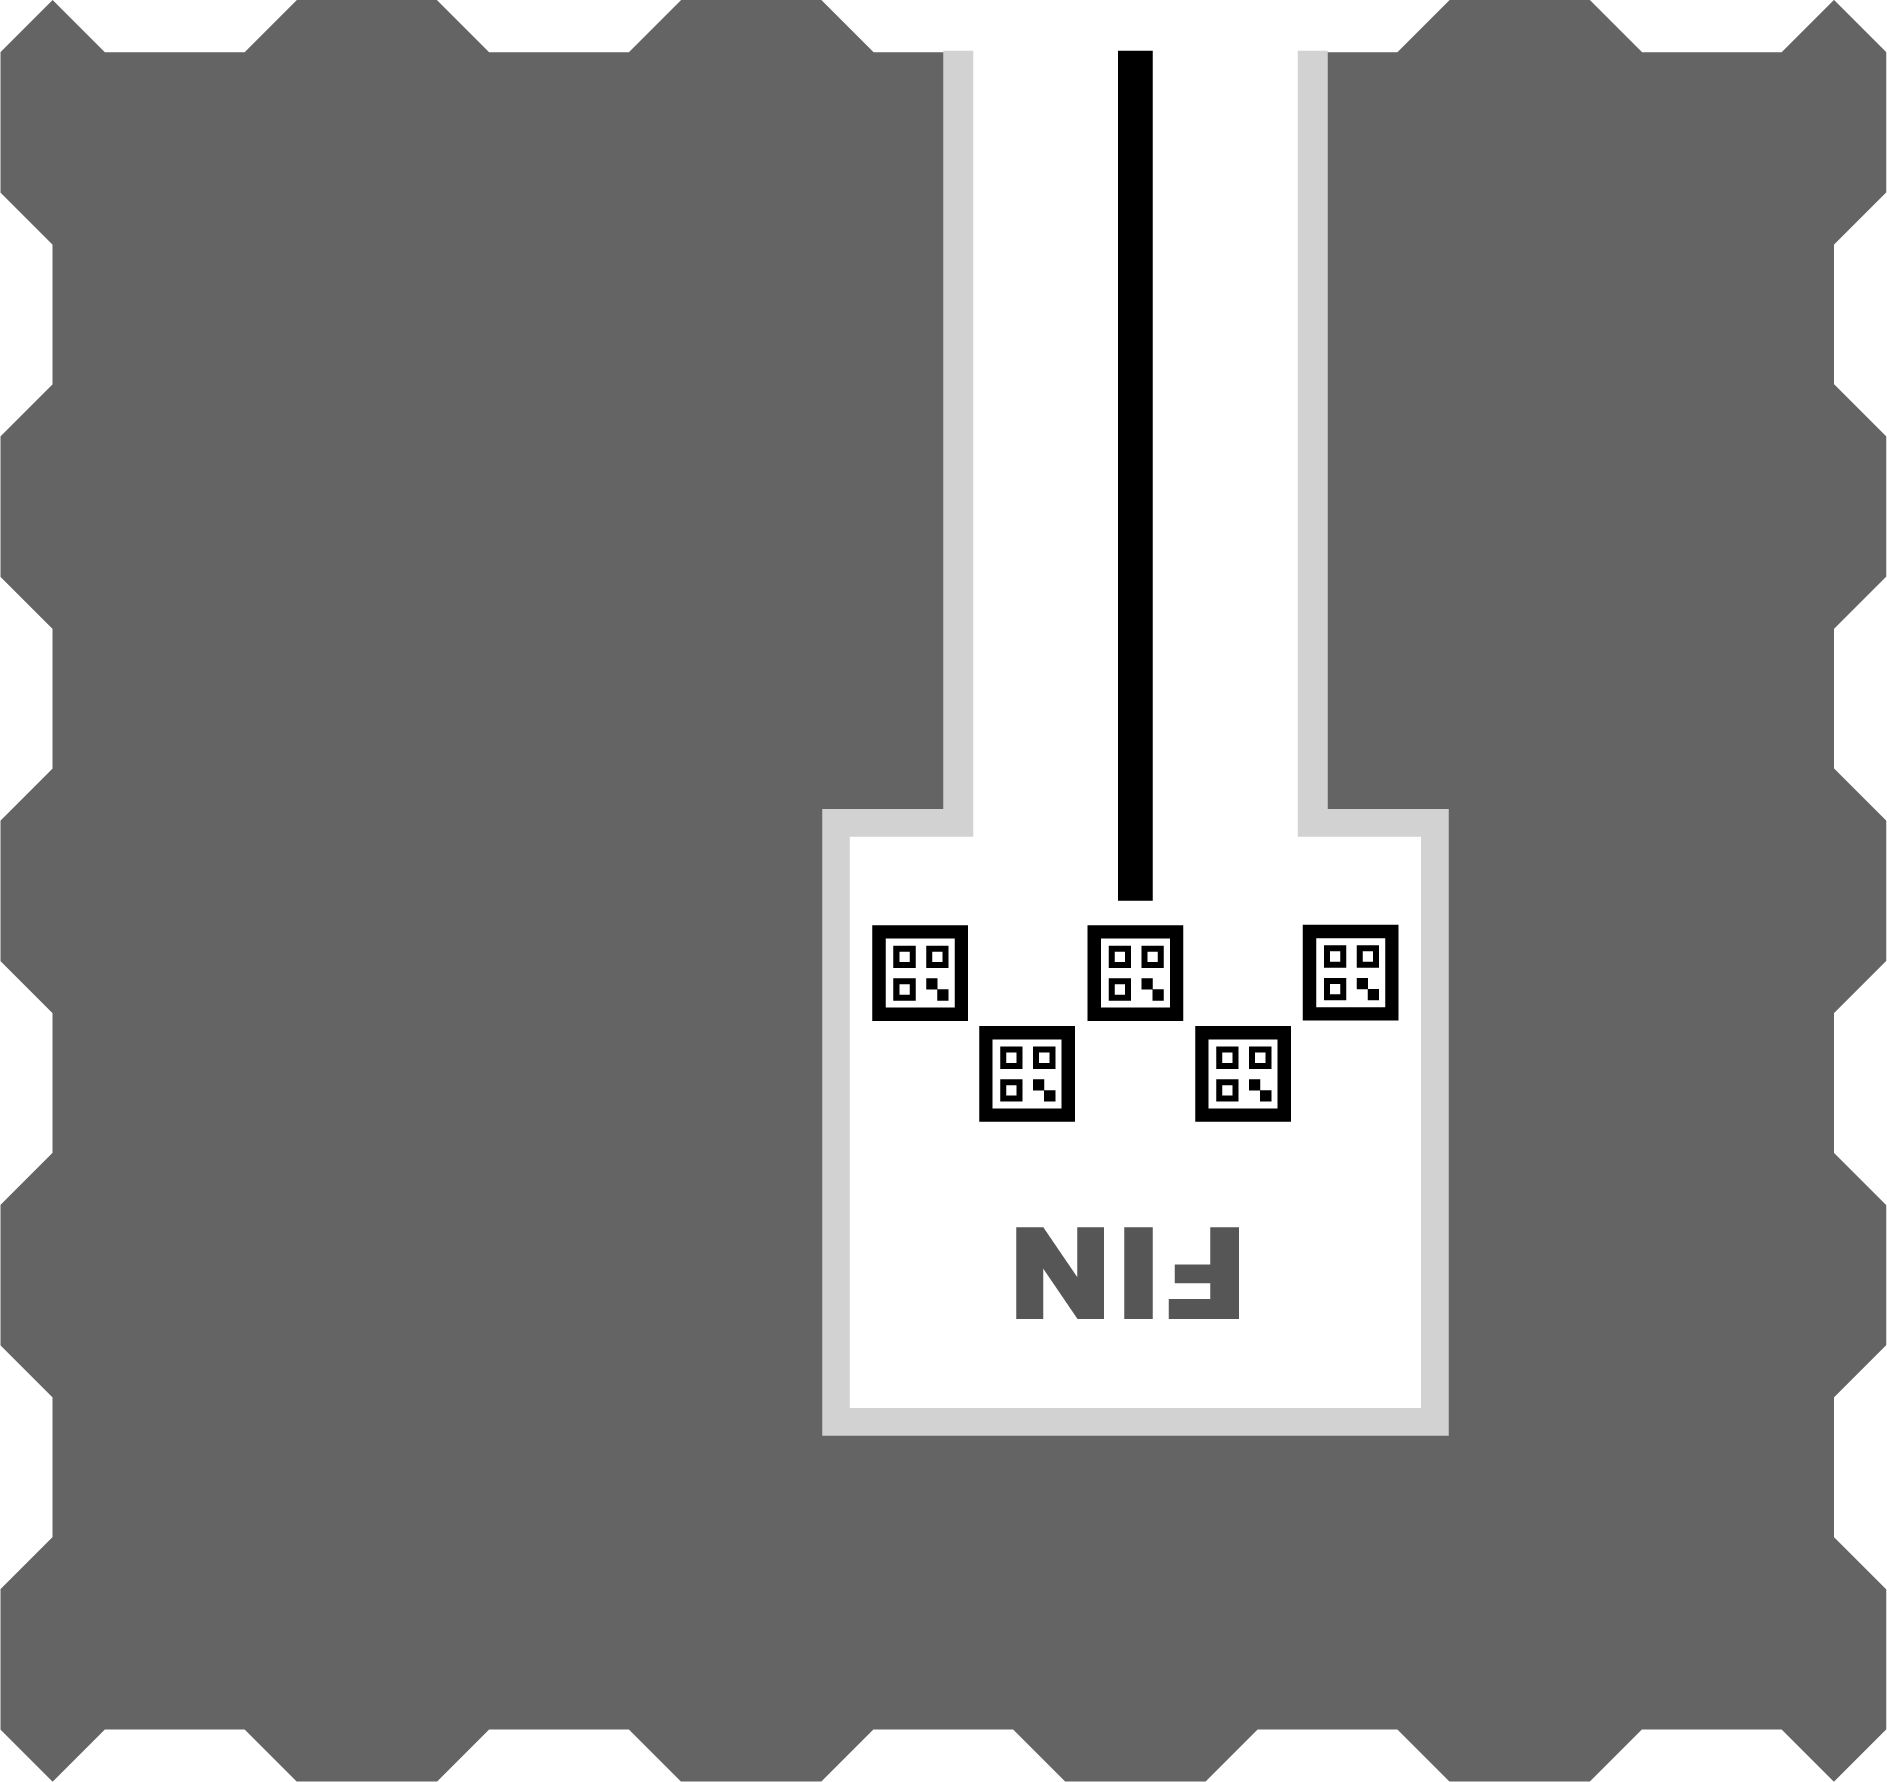
\includegraphics[width=\linewidth, angle=180]{images/tablero/tablero-end.png}
        \caption{Pieza del tablero con curva larga}
    \end{subfigure}

    \caption{Piezas del tablero}
    \label{fig:piezas-tablero}
\end{figure}

\FloatBarrier

\begin{itemize}
    \item Tarjetas correspondientes a cada elemento de la secuencia determinada por el docente. Cada tarjeta contiene un tag específico que luego será leído por Robotito en cada punto de parada, además de una sección libre donde el estudiante puede hacer dibujos, pegar una imagen o ubicar otro objeto arriba.
\end{itemize}

\begin{figure}[htbp]
    \centering

    \begin{subfigure}{0.20\textwidth}
        \centering
        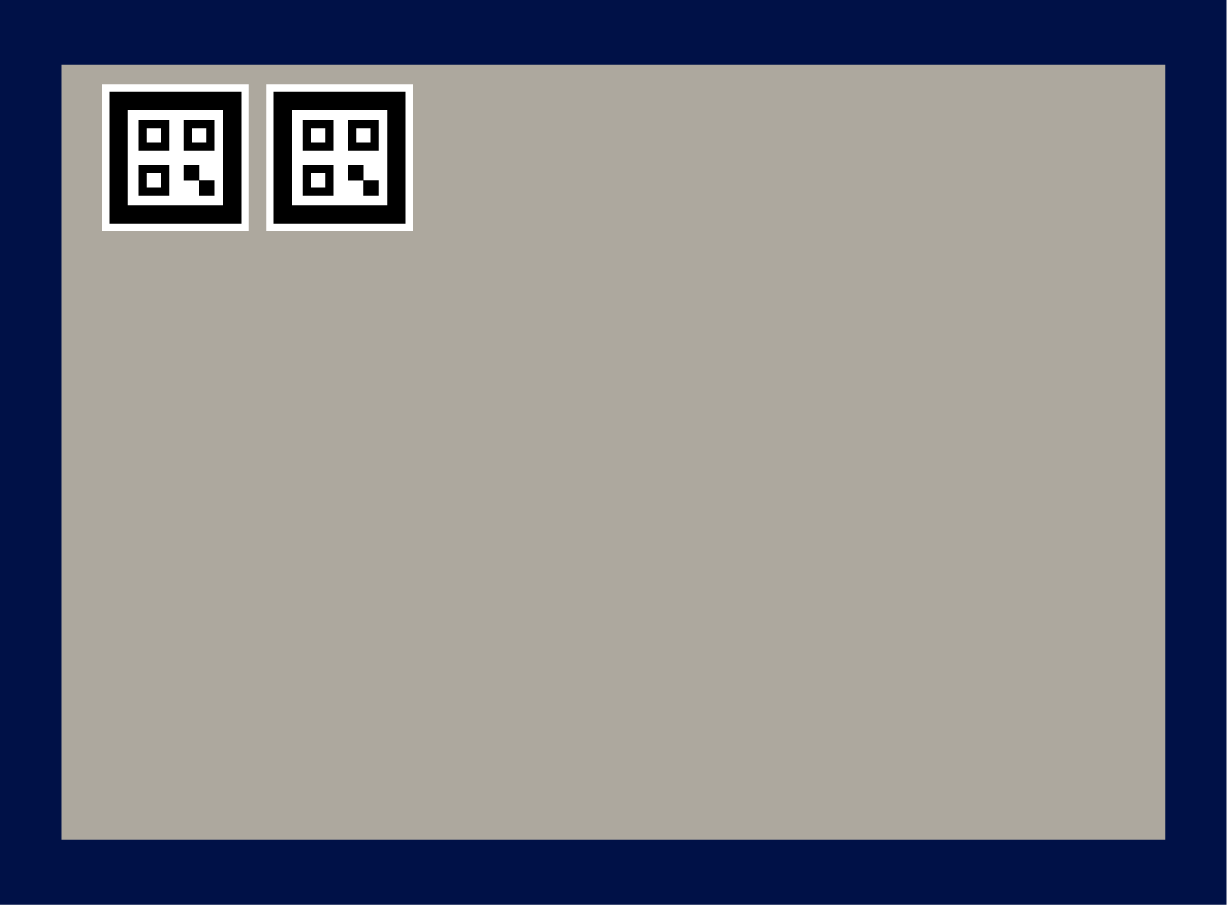
\includegraphics[width=\linewidth]{images/tablero/tarjeta-dibujo.png}
    \end{subfigure}

    \caption{Ejemplo de tarjeta con tags}
    \label{fig:tarjeta-tags}
\end{figure}

Cada pieza del tablero es un cuadrado encastrable de goma EVA de dimensiones 50cm x 50cm, con borde recto (sin encastre) en la zona donde se unen las líneas del recorrido (para evitar errores de lectura del robot), facilitando el armado y guardado por parte de docentes y alumnos. Además, la decisión de separar cada elemento del recorrido en distintas piezas agrega la posibilidad de crear recorridos distintos con curvas y rectas a lo largo del espacio en el que se utiliza.

Un ejemplo de recorrido completo se vería de la siguiente manera:

\begin{figure}[H]
    \centering

    \begin{subfigure}{0.75\textwidth}
        \centering
        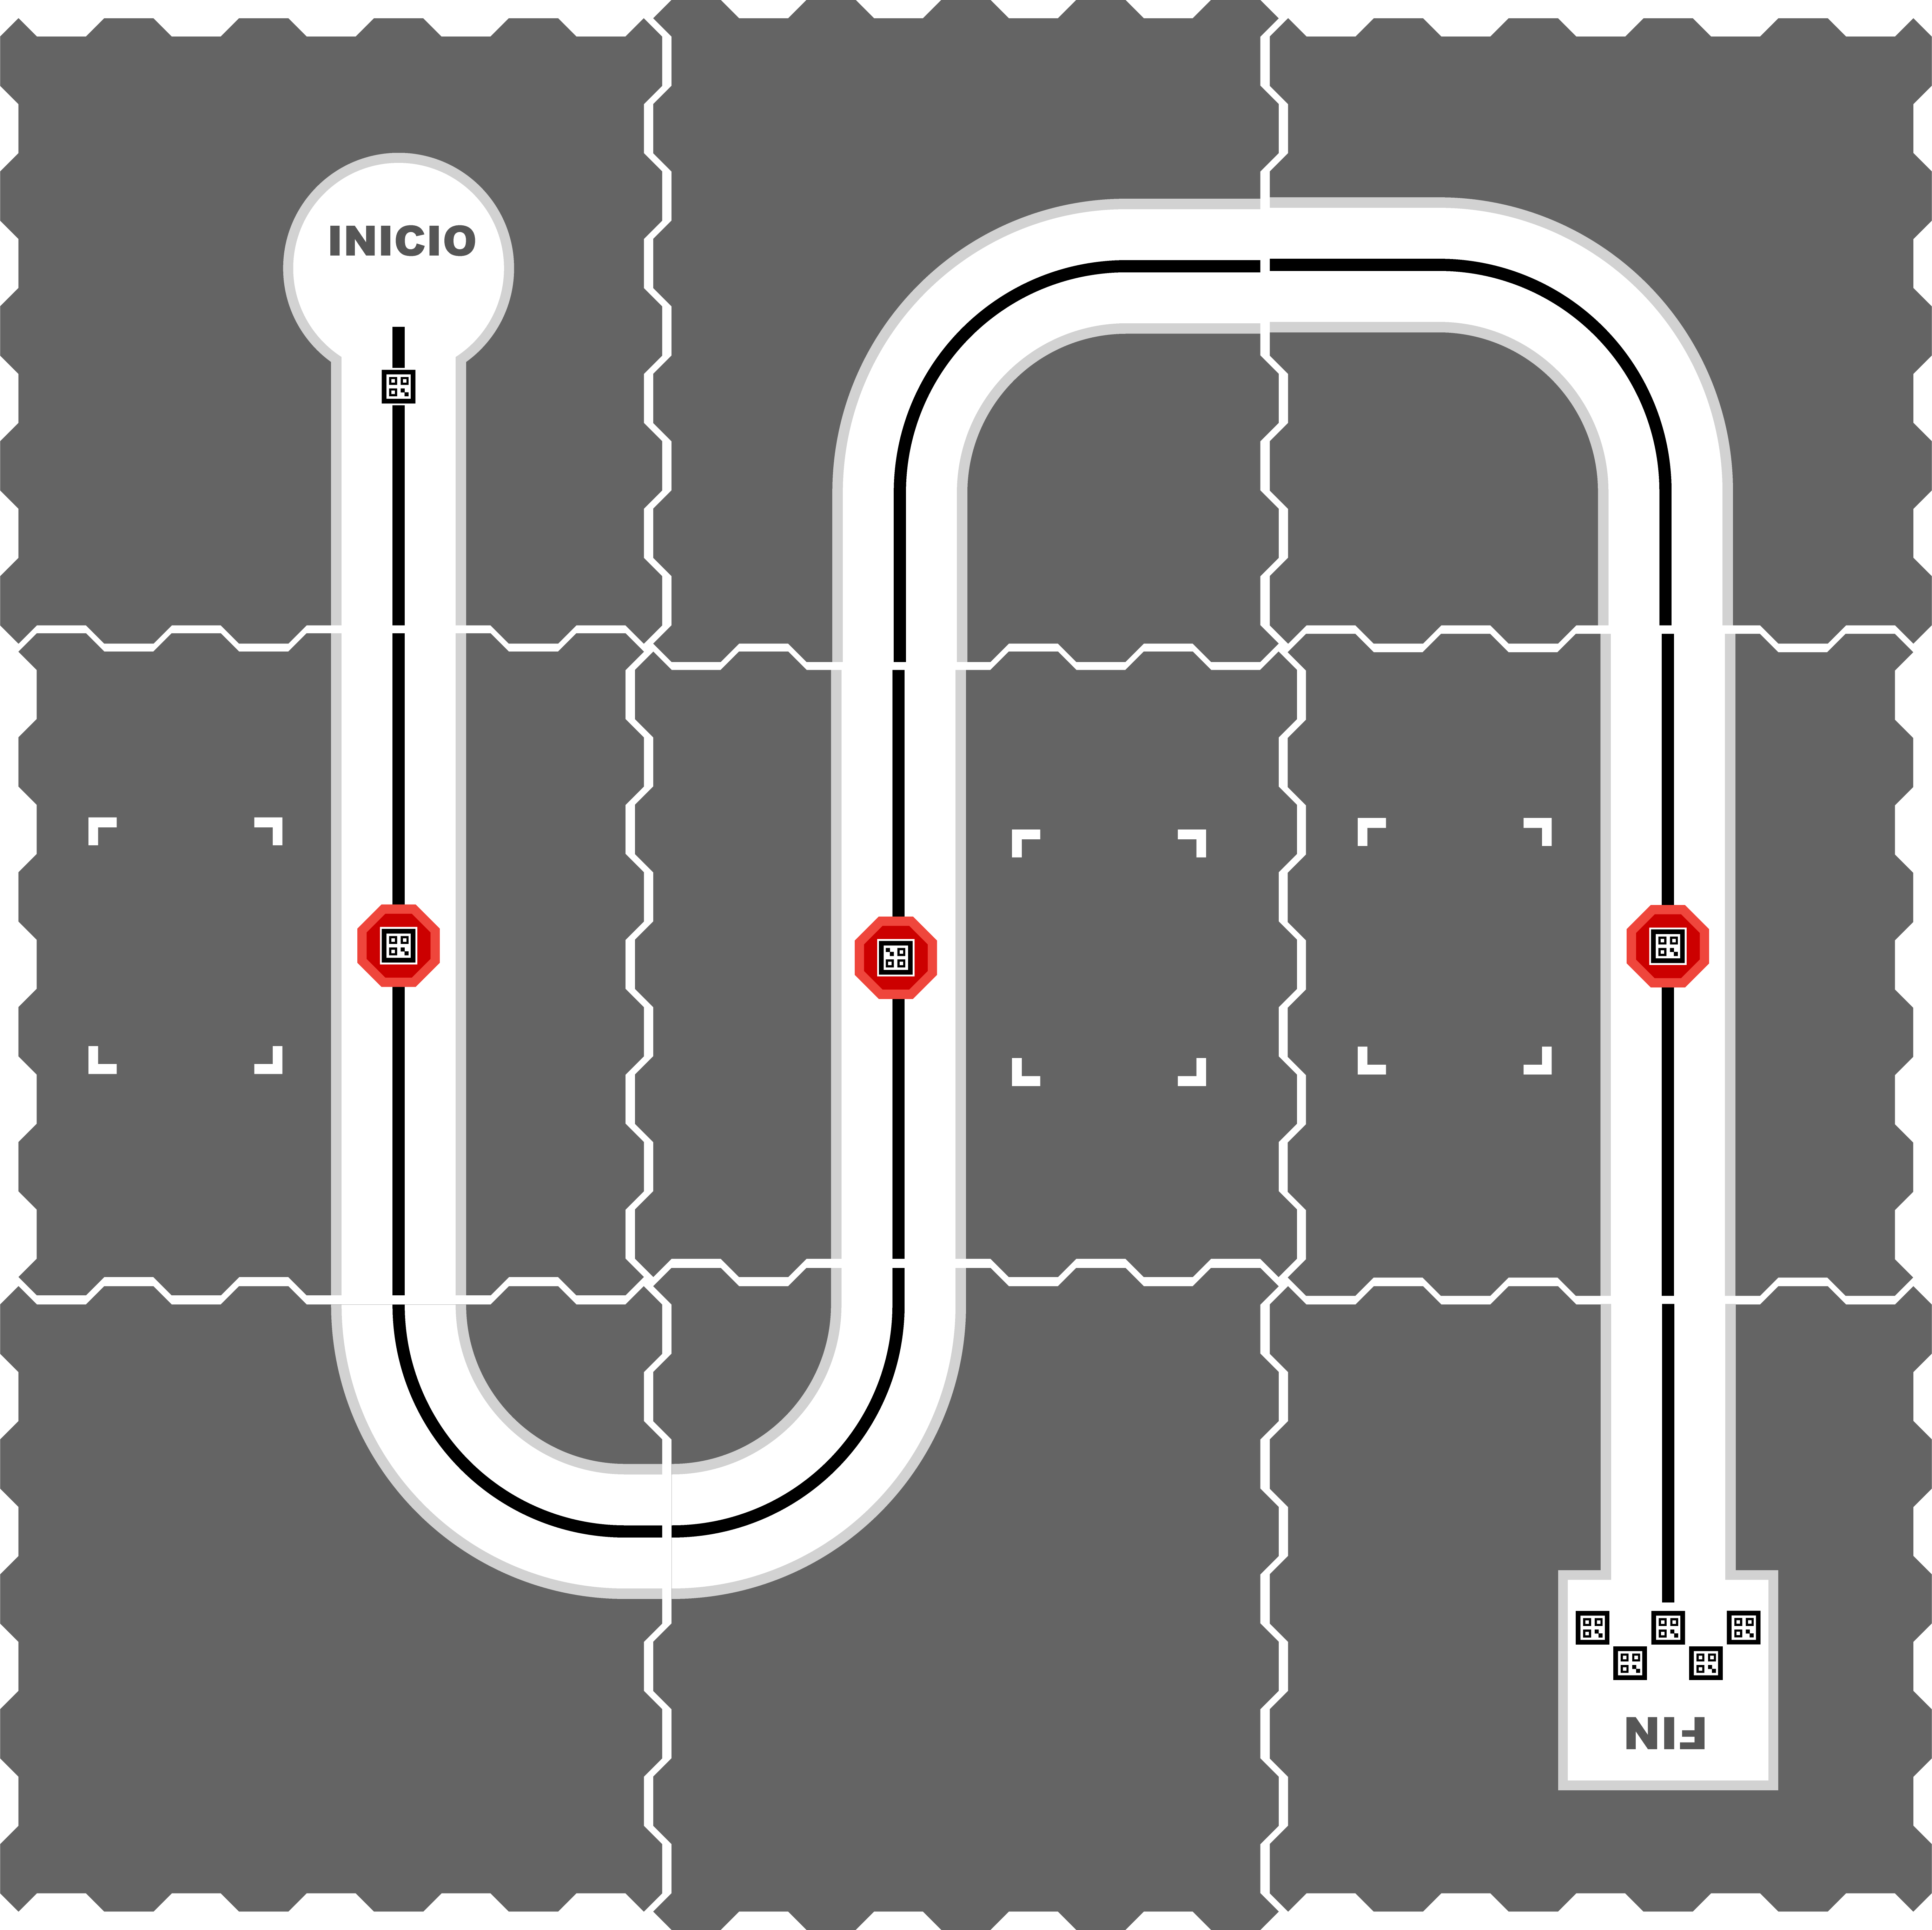
\includegraphics[width=\linewidth]{images/tablero/robotito-tablero-recorrido.png}
    \end{subfigure}

    \caption{Ejemplo de recorrido completo}
    \label{fig:recorrido-completo}
\end{figure}

Además de estos materiales, la actividad cuenta con dos tarjetas adicionales, cada una con un tag específico a ser leído por el robot. El funcionamiento de cada una se explica en la sección~\ref{subsec:recorrido-completo} (Ejecución del robot).

\begin{figure}[htbp]
    \centering
    \begin{subfigure}[t]{0.22\textwidth}
        \centering
        \vspace{0pt}
        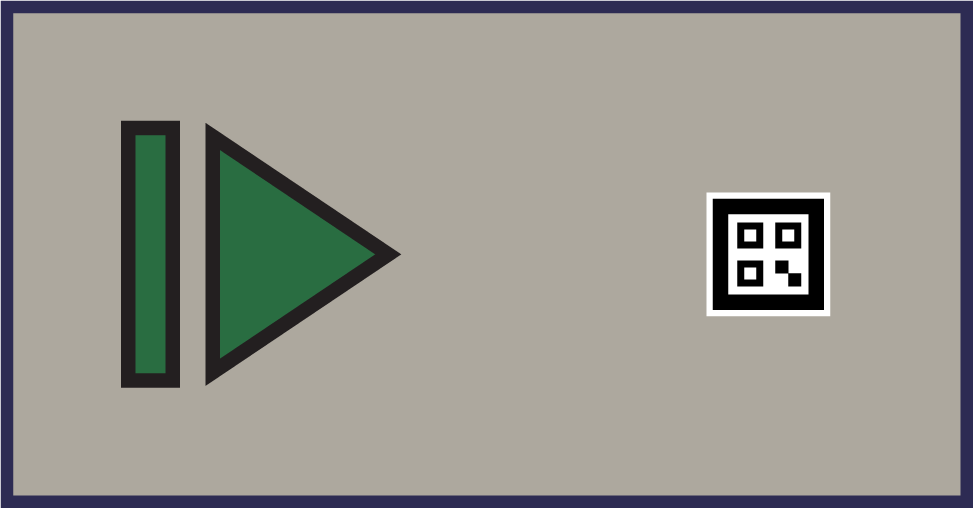
\includegraphics[width=\linewidth]{images/tablero/tarjeta-start.png}
        \caption{Tarjeta de Inicio}
        \label{subfig:tarjetas-control-inicio}
    \end{subfigure}
    \hspace{0.1\textwidth}
    \begin{subfigure}[t]{0.22\textwidth}
        \centering
        \vspace{0pt}
        
\includegraphics[width=\linewidth]{images/tablero/tarjeta-exit-config.png}
        \caption{Tarjeta para salir de modo de configuración}
        \label{subfig:tarjetas-control-config}
    \end{subfigure}

    \label{fig:tarjetas-control}
\end{figure}

\subsection{Desarrollo de la actividad}

Definidos los materiales, la actividad a desarrollar consiste en una serie de pasos. En primer lugar, el docente debe configurar previamente la secuencia que será verificada por Robotito en el recorrido. Esto se traduce a definir una lista ordenada de tags a ser leída por Robotito durante el recorrido (un tag de cada tarjeta a ubicar en el tablero) y enviarla al robot. Este paso es explicado con más detalle en la sección~\ref{sec:configurador-web}, correspondiente al configurador web. En resúmen, en esta parte el docente define qué tarjeta debe ir ubicada en qué lugar del recorrido.

Luego de configurada la actividad, en una instancia con alumnos el docente presenta el concepto de secuencia ordenada, poniendo como ejemplo secuencias que sean entendibles por niños de educación inicial, como las partes de un cuento conocido, las estaciones del año, pasos de la rutina diaria, o incluso una secuencia ordenada de números, entre otros.

Una vez presentados el concepto y ejemplos, se recomienda realizar una instancia de intercambio entre docente y alumnos en la que se presenta a Robotito y se habla brevemente sobre su aspecto, sus posibles funciones, relacionándolo con objetos de la vida cotidiana. De esta forma se puede presentar al grupo conceptos de robótica y pensamiento lógico, generando curiosidad e indagación. También se puede armar y hablar sobre el tablero, intentando llegar a un acuerdo sobre qué le parece al grupo que representa toda la actividad, así como mostrar las tarjetas y relacionar todo lo hablado con el concepto de secuencia ordenada. 

Luego de presentados Robotito, el tablero y las tarjetas, y vinculado todo con el concepto de secuencia ordenada, el grupo debe ponerse de acuerdo en una secuencia específica a representar con las tarjetas, que luego serán ubicadas en el tablero y verificadas por el robot durante el recorrido. Para esto se pueden hacer dibujos (correspondientes a cada paso de la secuencia) en papeles que luego serán pegados en la zona libre de cada tarjeta, dibujos sobre la misma tarjeta, o incluso ubicar objetos arriba de cada una. El punto importante de este paso a tener en cuenta por el docente es que la relación entre el dibujo u objeto y la tarjeta debe ser correcta con respecto a la posición de cada uno en la secuencia. Por ejemplo, el dibujo correspondiente al primer paso de la secuencia debe estar pegado sobre la tarjeta que contenga el primer tag de la secuencia configurada, el objeto correspondiente al segundo paso de la secuencia debe estar ubicado sobre la tarjeta que contenga el segundo tag de la secuencia configurada, y así sucesivamente.

Una vez realizado el vínculo correcto por parte del docente entre tarjetas y pasos de la secuencia representados por los estudiantes, debe haber una instancia compartida en la que los estudiantes deben ubicar cada tarjeta (con su dibujo u objeto) en cada uno de los puntos de parada del recorrido armado.

Terminado el paso anterior, se ubica a Robotito en el punto de partida y se da comienzo al recorrido completo, en el que el robot se detiene en cada punto de parada para verificar si el tag de la tarjeta ubicada en ese punto corresponde a la posición del mismo en la secuencia. Si bien en este paso el robot está leyendo la información de los tags, al agregar un dibujo u objeto en cada tarjeta se genera la sensación de que el robot en realidad está mirando la imagen y no el tag (en el capítulo de Experimentación se detallan las actividades realizadas y las reacciones obtenidas). Luego de obtenida y procesada la información del tag correspondiente a la tarjeta en cada punto de parada, el robot reacciona con una retroalimentación luminosa dependiendo de si el elemento se encuentra en la posición correcta (luz verde) o incorrecta (luz roja) de la secuencia a verificar. 

Finalmente, al llegar al punto de fin del tablero, el robot devuelve una retroalimentación general del recorrido, con el objetivo de informar si este fue correcto o si hubo errores, indicando cuáles elementos leídos no se encontraban en la posición correcta. Esto permite que el recorrido se realice más de una vez, reubicando las tarjetas para indagar sobre cuál debería ser el comportamiento del robot en cada caso.

\subsection{Ejecución del robot}
\label{subsec:recorrido-completo}

Al encender Robotito, este se encuentra en modo ``Configuración'', con su anillo LED parpadeando en color azul. En este paso es posible conectarse al robot a través del protocolo BLE utilizando el configurador web y transmitir datos de secuencia esperada entre ambos. En caso de querer empezar el recorrido, el robot se debe ubicar en el punto de inicio del tablero apuntando la cámara hacia la línea del recorrido, y luego mostrarle (a la cámara) la tarjeta correspondiente a ``salir de modo Configuración'' (\ref{subfig:tarjetas-control-config}).

A partir de ahora Robotito se encuentra en modo ``Esperando Inicio'' (con su anillo LED parpadeando en color blanco). Para empezar el recorrido se debe mostrar la tarjeta de Inicio (\ref{subfig:tarjetas-control-inicio}), y el robot empezará a moverse siguiendo la línea. \\

\textbf{Nota:} Si durante el recorrido Robotito es levantado del tablero o pierde la línea que venía siguiendo, se pondrá automáticamente en modo ``Pausa'', con su anillo LED parpadeando en color amarillo. En este modo el robot recuerda la secuencia leída y verificada hasta el momento, por lo que solamente hay que reubicarlo en el lugar del tablero donde se perdió o levantó (con la cámara apuntando hacia la línea), y mostrar la tarjeta de Inicio para que este retome el recorrido. \\

Como se mencionó anteriormente, los puntos de parada se representan con un tag específico que el robot reconoce durante su avance.

\begin{figure}[htbp]
    \centering

    \begin{subfigure}{0.20\textwidth}
        \centering
        
\includegraphics[width=\linewidth]{images/tablero/stop-qr.png}
    \end{subfigure}

    \caption{Ejemplo de punto de parada}
    \label{fig:stop-qr}
\end{figure}

Se toma la decisión de representar estos puntos de parada de manera similar a una señal de tránsito ``PARE'' roja, como forma de hacer su significado más intuitivo, relacionable con el día a día, y agregar color al recorrido. Luego de realizar varias pruebas se agrega una segunda instancia del mismo tag dentro de la figura para evitar errores de lectura del robot, en caso que este no lea la primera.

Una vez leído el tag correspondiente al punto de parada, el robot detiene su avance y empieza a rotar en sentido horario, hasta encontrar el tag de la tarjeta ubicada por el grupo en la zona específica. Con el objetivo de cumplir con que la tarjeta ubicada siempre se encuentre ``a la derecha'' del robot, se diseñan las piezas del tablero de manera que siempre se encastren de la misma forma, empezando con la pieza de ``Inicio'', seguida por rectas y curvas que solamente se encastrarán dejando el área específica para ubicar la tarjeta del lado derecho del recorrido, finalizando con la pieza de ``Fin''.

De igual manera que con los tags del punto de parada, se ubican dos tags iguales en la esquina de cada tarjeta (como se puede observar en \ref{fig:tarjeta-tags}), evitando errores de lectura del robot. Una vez leído alguno de los dos tags de la tarjeta, Robotito ``pensará'' brevemente (modo representado por su anillo LED prendiéndose progresivamente con luz blanca hasta completar el anillo, también pensado para darle al grupo una representación visual de lo que está haciendo el robot que, en este caso, significa la validación en tiempo real de la secuencia) y decidirá si la tarjeta leída se encuentra en la posición correcta o no. Si la posición es la tarjeta es correcta, el anillo LED se encenderá completamente con luz verde. En el caso incorrecto, se encenderá con luz roja. 

El feedback luminoso se mantiene por un breve período de tiempo, luego se apaga y el robot empieza su movimiento de rotación, esta vez en sentido antihorario buscando nuevamente los tags del punto de parada. Una vez encontrado nuevamente el tag, Robotito sigue su recorrido por la línea del tablero.

Este proceso se repite la cantidad de veces que sea necesaria, según la cantidad de puntos de parada haya en el recorrido completo, finalmente llegando al punto de fin.

\begin{figure}[htbp]
    \centering

    \begin{subfigure}{0.50\textwidth}
        \centering
        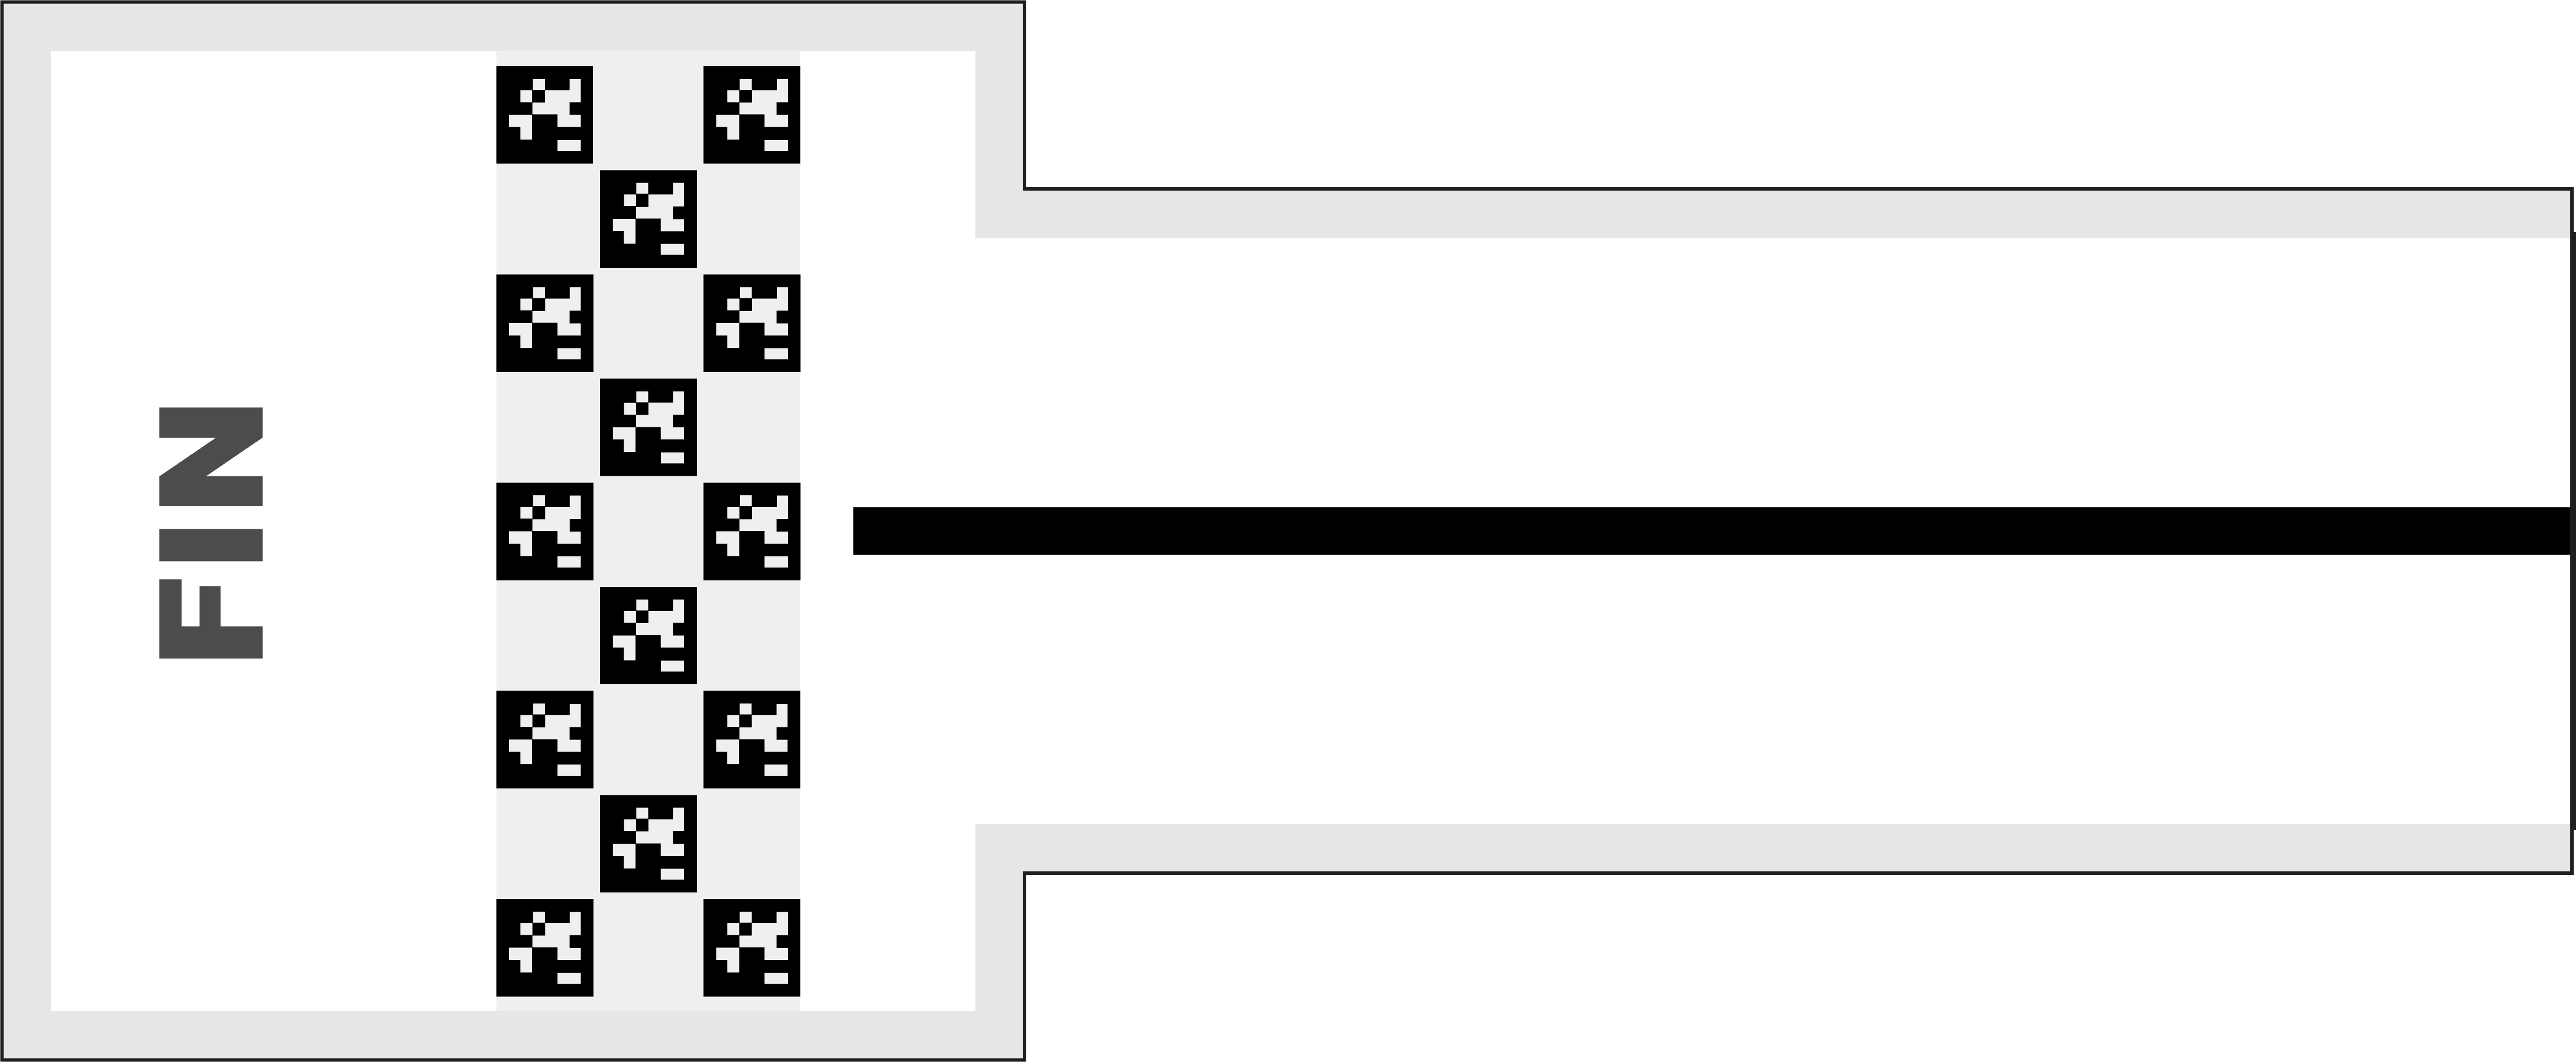
\includegraphics[width=\linewidth, angle=180]{images/tablero/tablero-end-real.png}
    \end{subfigure}

    \caption{Punto de fin utilizado en las pruebas}
    \label{fig:tablero-fin-real}
\end{figure}

Como se puede observar en la figura~\ref{fig:tablero-fin-real}, el final del recorrido se representa por varias instancias del mismo tag formando una figura similar a una bandera de fin utilizada en carreras. Nuevamente, el objetivo es hacer la actividad intuitiva y relacionable con situaciones y símbolos del dia a día.

Al realizar la lectura de alguno de los tags ubicados en el punto de fin del recorrido, Robotito evalúa si todas las estaciones fueron visitadas en el orden correcto y retorna feedback de la verificación completa. En caso que la secuencia haya tenido errores de posición, Robotito se detiene y muestra en su anillo LED el resultado de cada posición en los colores rojo o verde, representando error o acierto, sucesivamente.

\begin{figure}[htbp]
    \centering

    \begin{subfigure}{0.25\textwidth}
        \centering
        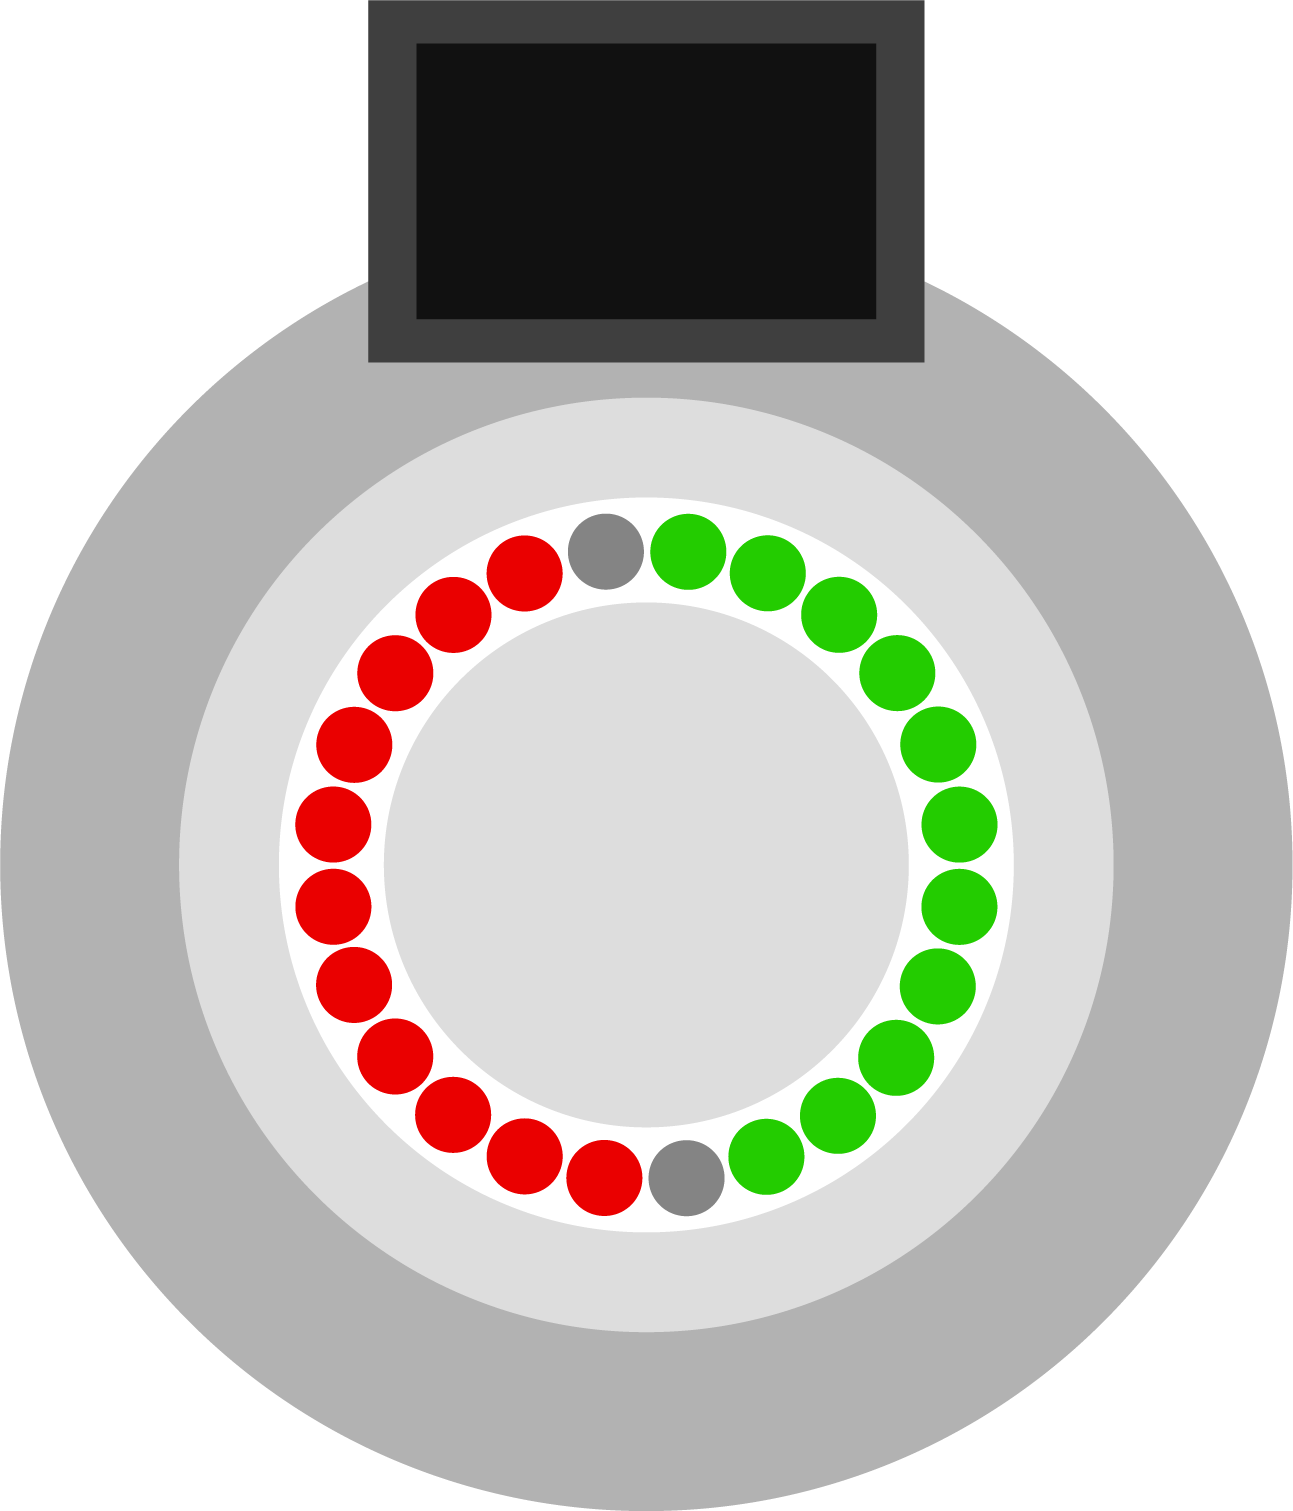
\includegraphics[width=\linewidth]{images/robotito/robotito-segmento-1.png}
        \caption{Feedback final con un error, dos puntos de parada en total}
    \end{subfigure}
    \hfill
    \begin{subfigure}{0.25\textwidth}
        \centering
        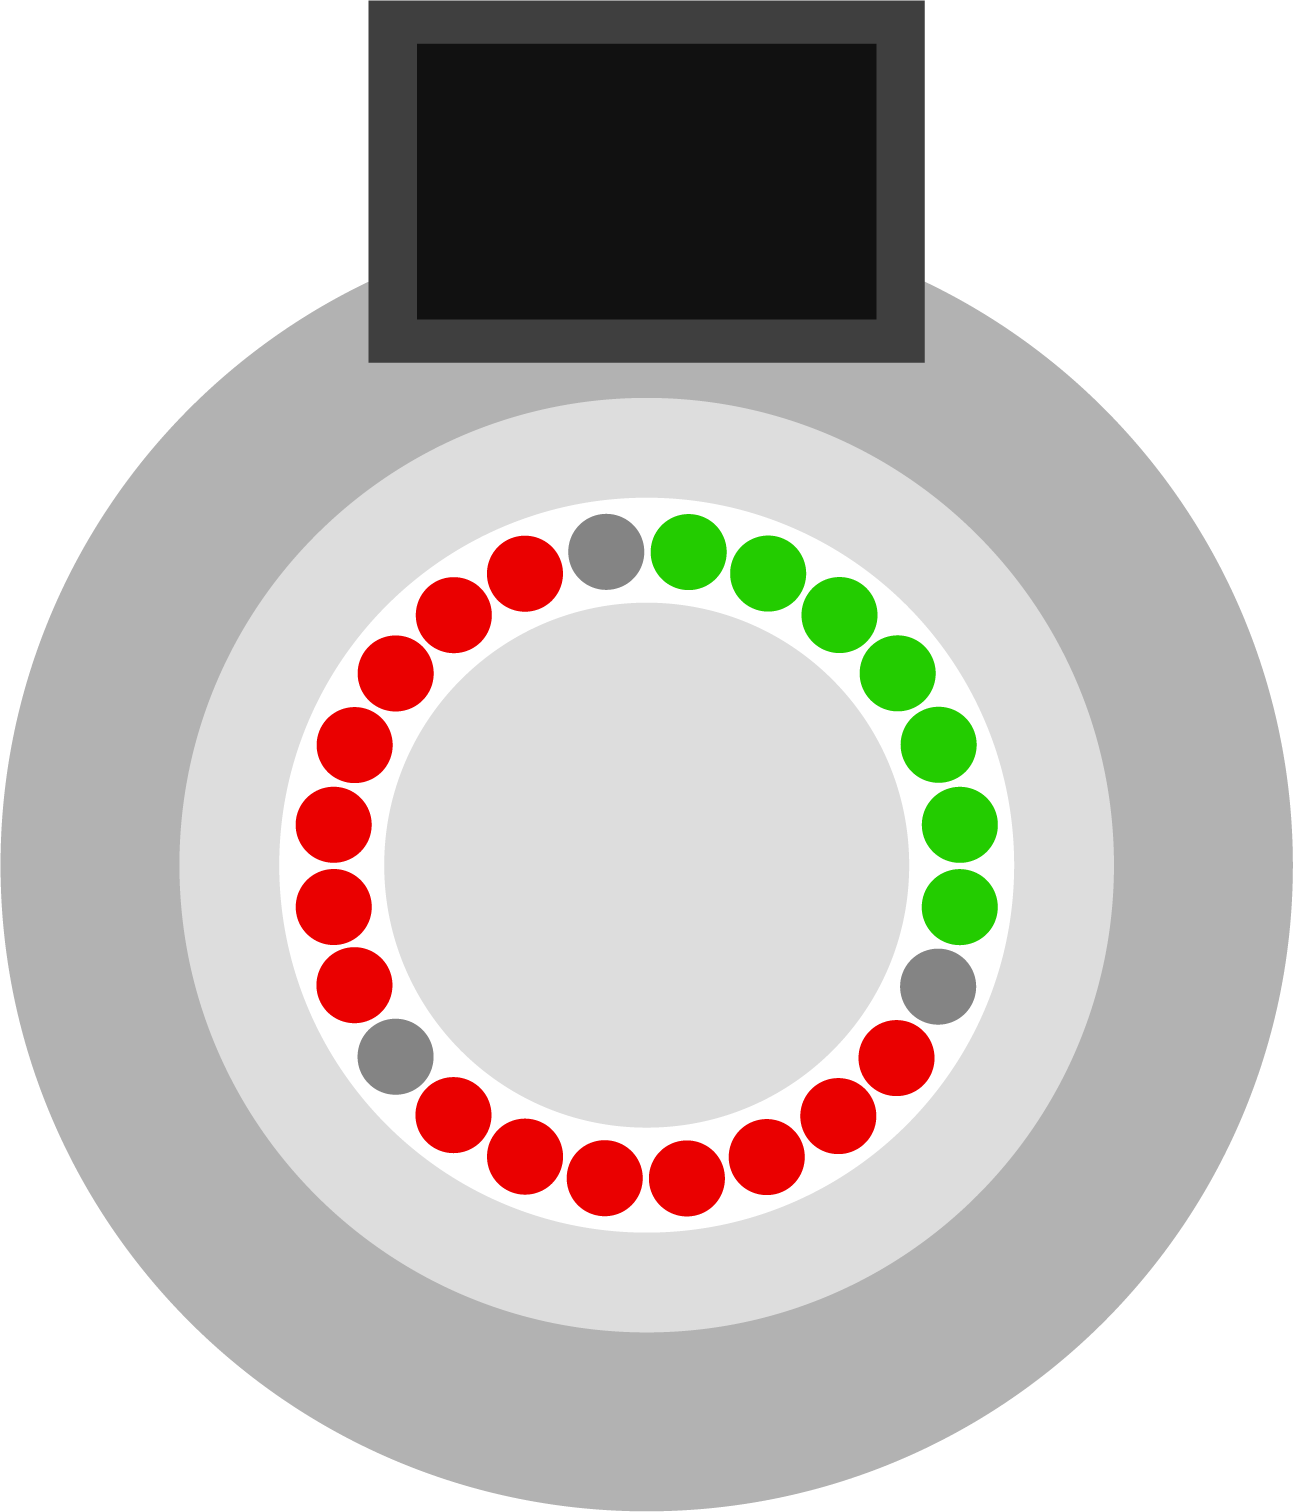
\includegraphics[width=\linewidth]{images/robotito/robotito-segmento-2.png}
        \caption{Feedback final con dos errores, tres puntos de parada en total}
    \end{subfigure}
    \hfill
    \begin{subfigure}{0.25\textwidth}
        \centering
        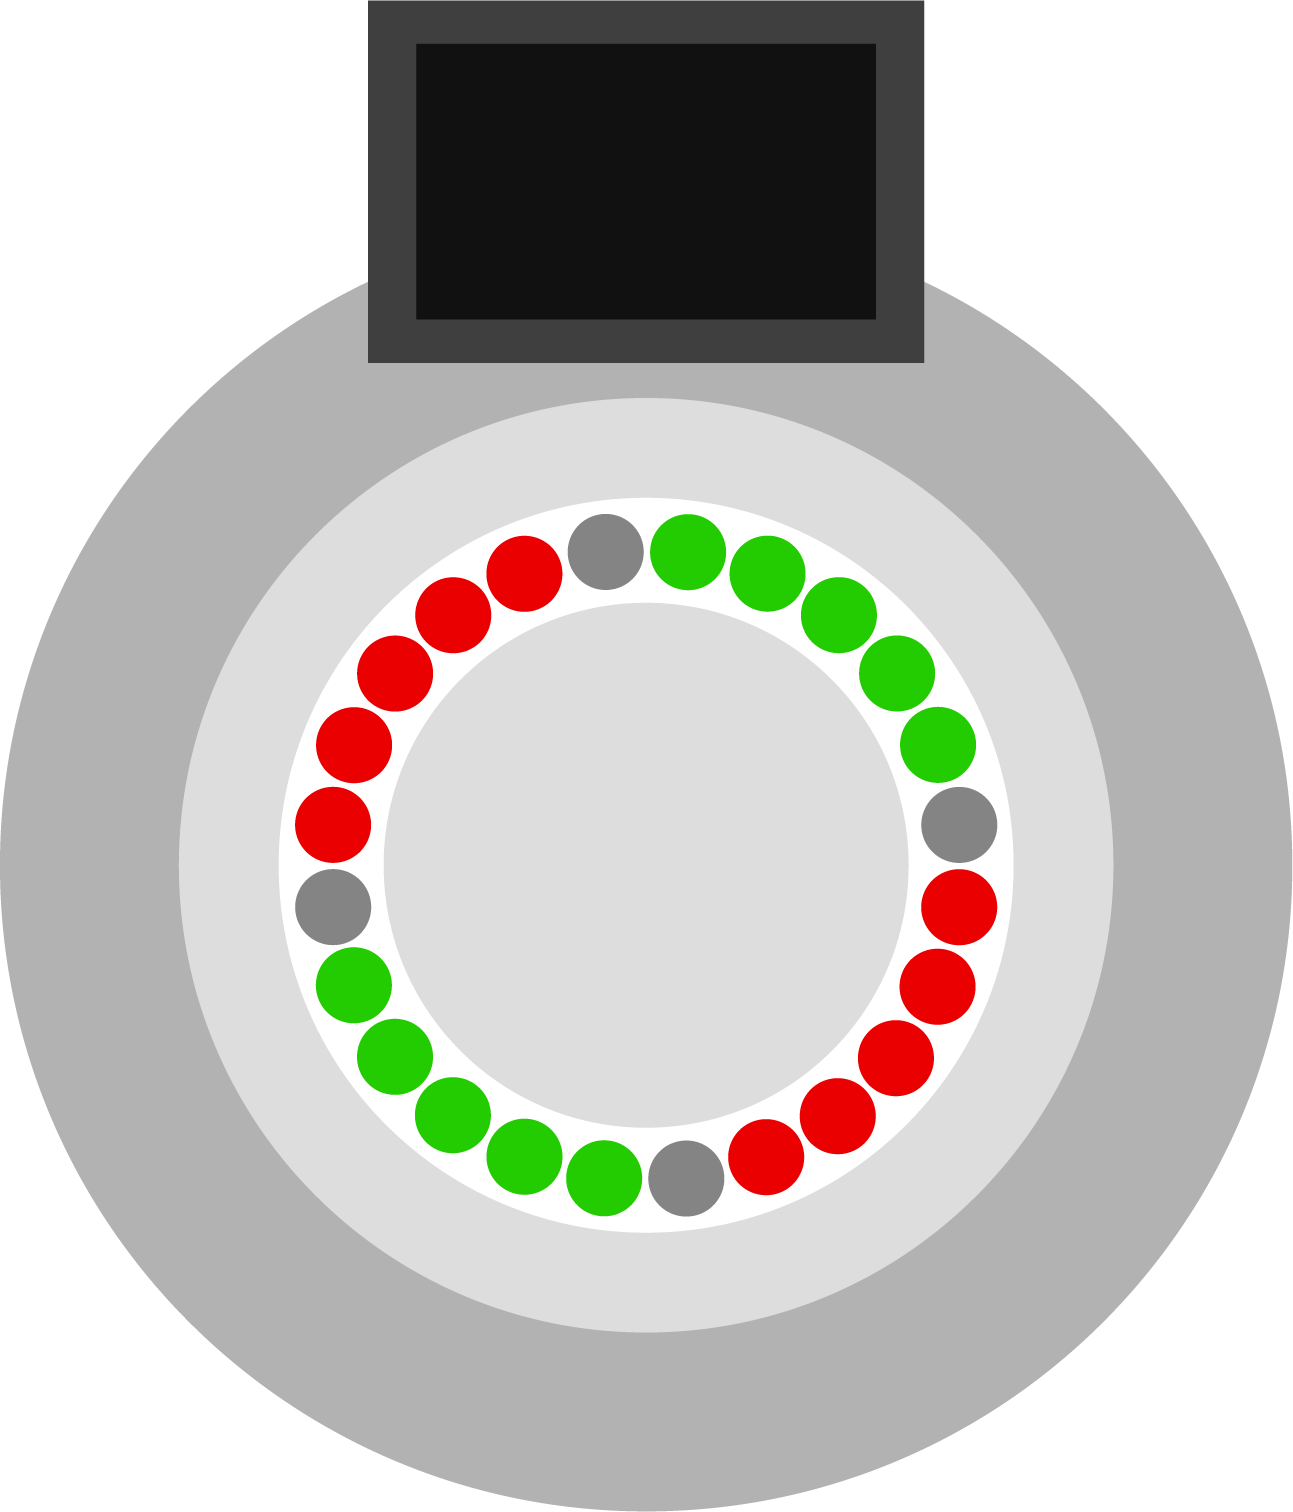
\includegraphics[width=\linewidth]{images/robotito/robotito-segmento-3.png}
        \caption{Feedback final con dos errores, cuatro puntos de parada en total}
    \end{subfigure}

    \caption{Ejemplos de feedback final con error, con distintas cantidades de puntos de parada en el recorrido}
    \label{fig:feedback-final}
\end{figure}

\FloatBarrier

En caso que la secuencia verificada sea correcta, Robotito sigue avanzando brevemente (pasando la zona representada por la ``bandera final'' de tags), y luego realiza giros en forma de ``festejo'' con su anillo LED encendido completamente en color verde.

Finalmente, en caso de querer reiniciar el recorrido, Robotito debe ser ubicado en el punto de Inicio del tablero, que además cuenta con un tag específico para reiniciar la actividad. Una vez leído ese tag, el historial de la secuencia validada hasta ese momento se descarta y el robot vuelve a modo ``Esperando Inicio'' (con su anillo LED parpadeando con luz blanca) listo para empezar un nuevo recorrido.

\begin{figure}[htbp]
    \centering

    \begin{subfigure}{0.50\textwidth}
        \centering
        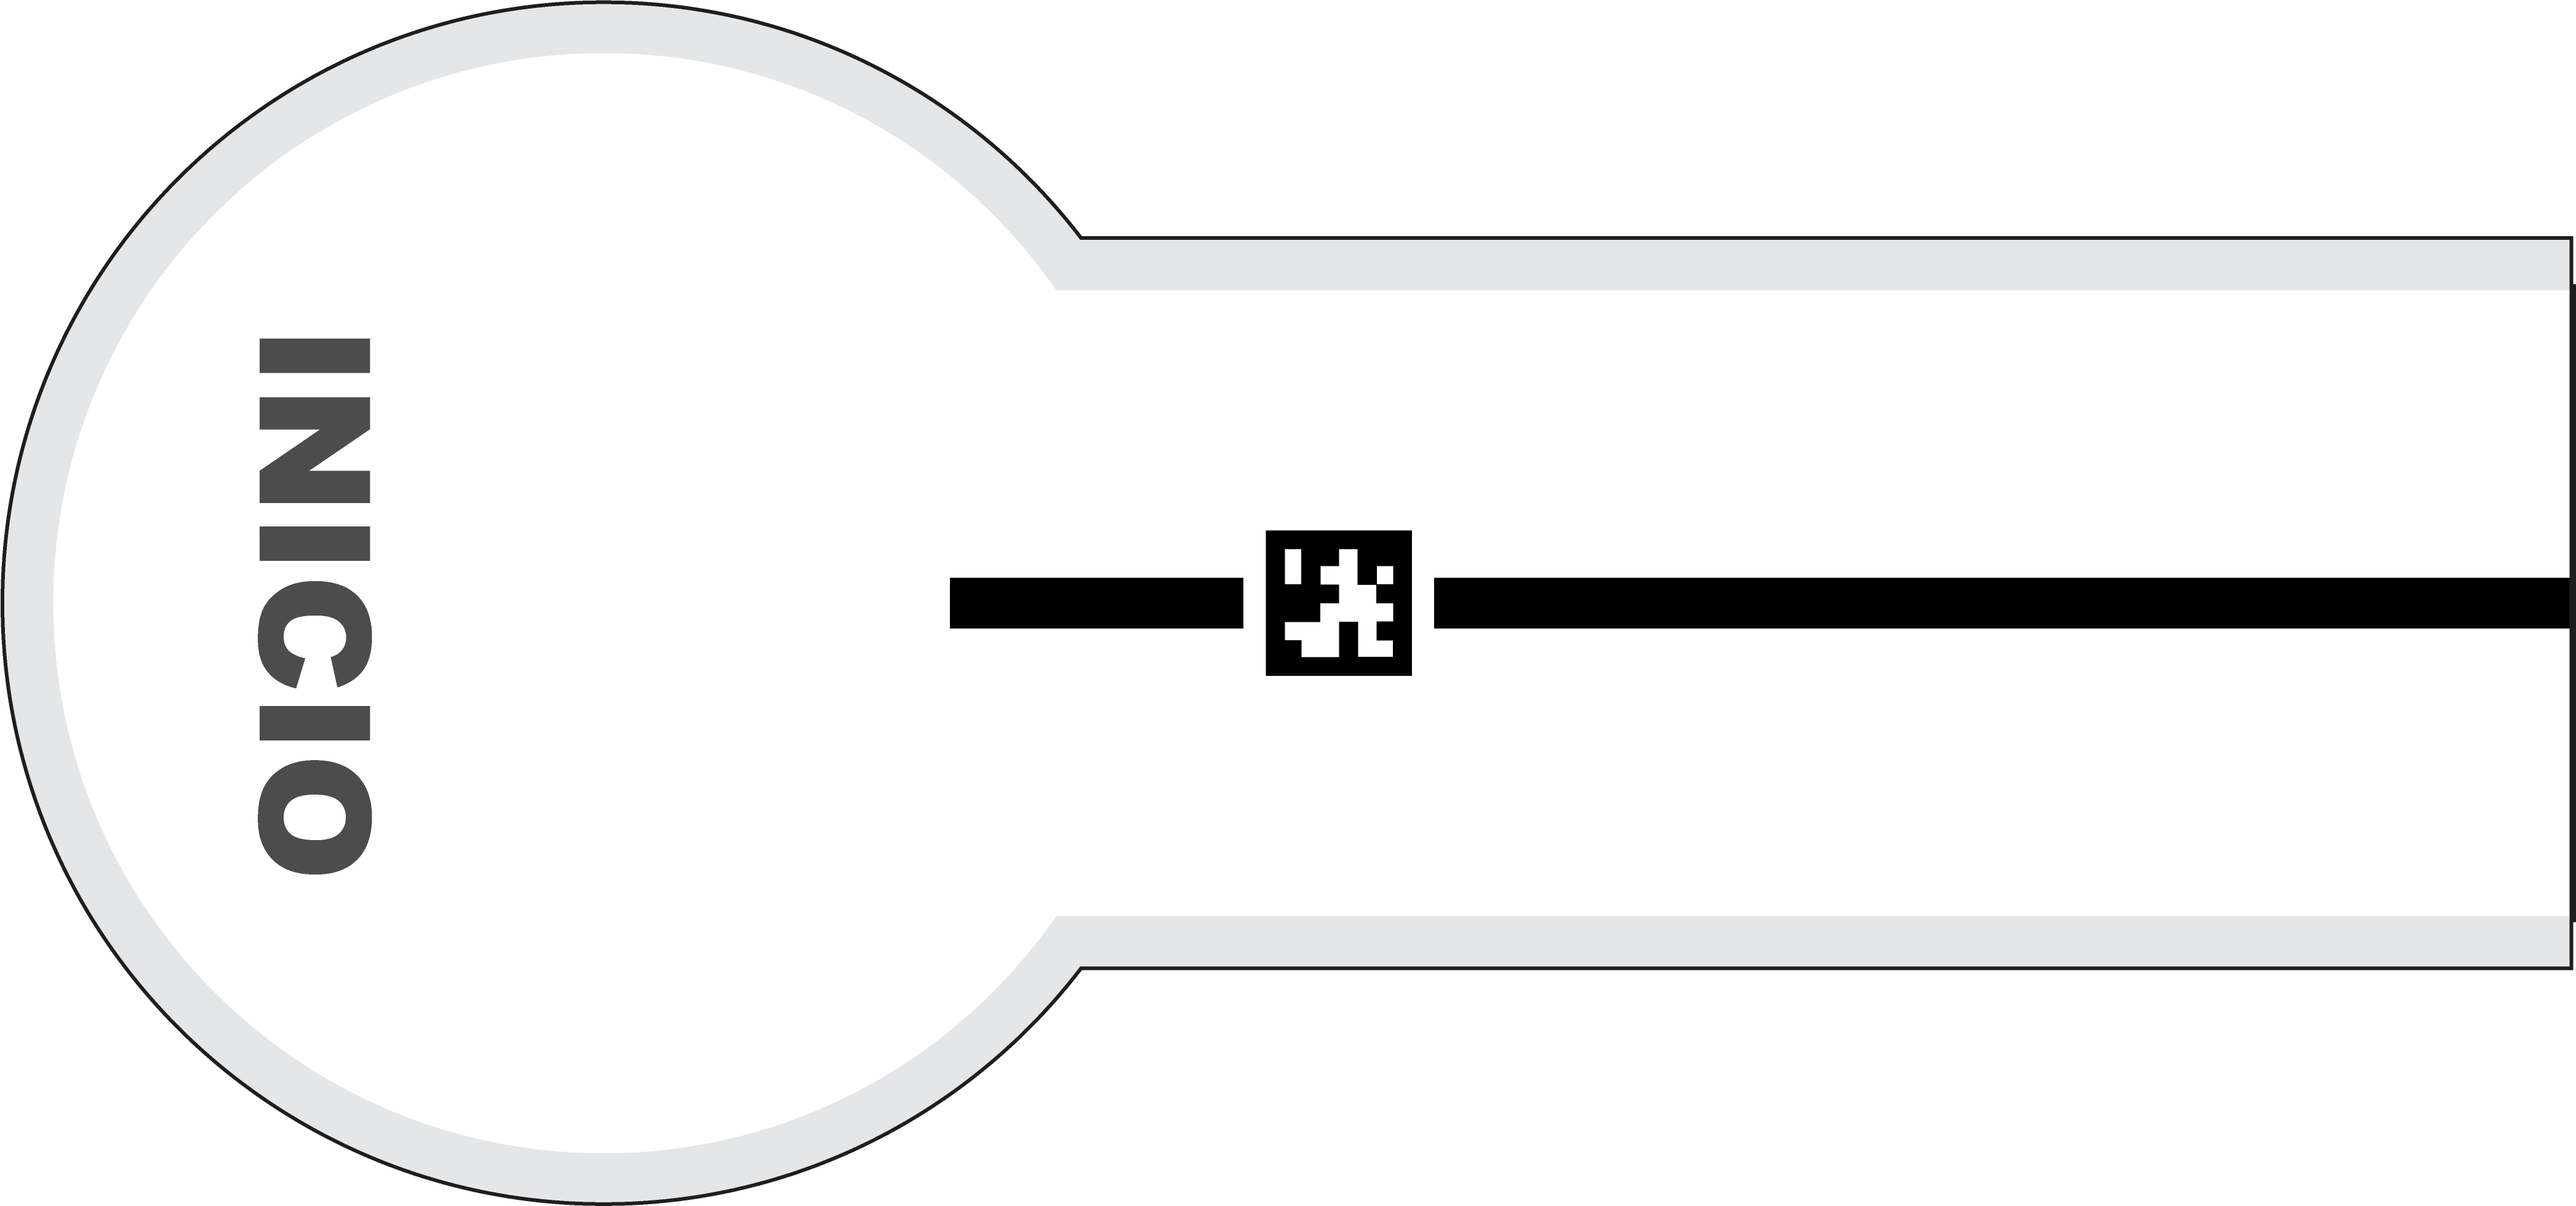
\includegraphics[width=\linewidth]{images/tablero/tablero-start-real.png}
    \end{subfigure}

    \caption{Punto de inicio utilizado en las pruebas (con tag de reinicio)}
    \label{fig:tablero-start-real}
\end{figure}

% TODO agregar info sobre ejecución del robot en el juego


% ================== FIN CAP 3 (ANALISIS & DISEÑO)  ==================


% parte central
\chapter{Implementación de la solución}
\label{cap:implementacion}
% ===== HUSKYLENS =====
\section{Módulo de percepción visual con HuskyLens}

Como se mencionó en capítulos anteriores, uno de los objetivos es incorporar una cámara a Robotito para ampliar sus funcionalidades. Para seleccionar la opción más adecuada, se realizó un análisis de las cámaras disponibles en el mercado.

Las características principales que se buscan son la compatibilidad con la placa ESP32, la capacidad de detectar colores, objetos y líneas, y la disponibilidad de estos algoritmos implementados directamente en la cámara para reducir el tiempo de integración. Además, se considera importante que la cámara tenga un costo y un tamaño adecuados, este úlitmo con el objetivo para poder instalarla en la parte superior del robot.

A partir de estos criterios, se identificaron varias alternativas disponibles en el mercado, las cuales se describen en Anexo \ref{sec:tabla_comparativa_camaras}. Luego de evaluar cada opción, se seleccionó la cámara HuskyLens, dado que cumple con todos los requisitos establecidos. 

Antes de describir su integración con Robotito, se presenta a continuación el funcionamiento general de la cámara: los algoritmos de visión que ofrece y la forma en que representa la información que detecta.

\subsection{Funcionamiento de HuskyLens}

\subsubsection{Algoritmos de visión}

HuskyLens incorpora distintos algoritmos de visión artificial que permiten realizar diferentes tareas, como el reconocimiento de objetos, colores y rostros, el seguimiento de líneas y la detección de marcadores visuales. Cada algoritmo procesa las imágenes capturadas por la cámara y devuelve la información correspondiente a las detecciones realizadas.

En este trabajo se utilizaron únicamente dos de estos algoritmos:

\begin{itemize}
    \item \textbf{Seguimiento de líneas (\textit{Line Tracking}):} permite detectar una línea dentro del campo visual de la cámara y seguir su recorrido. Este algoritmo se utiliza para implementar el seguimiento de líneas por parte de Robotito.

    \item \textbf{Reconocimiento de marcadores visuales (\textit{Tag Recognition}):} permite detectar marcadores de tipo \textit{AprilTag}. Para cada tag detectado, la cámara devuelve un identificador único y su posición dentro de la imagen, lo que permite al robot reconocerlo y localizarlo.
\end{itemize}

La información devuelta por estos algoritmos se representa mediante dos tipos de estructuras, las cuales se describen a continuación.

\subsubsection{Representación de las detecciones}

La información generada por los algoritmos de HuskyLens se representa mediante dos tipos de estructuras: \textit{bloques} (\textit{BLOCK}) y \textit{flechas} (\textit{ARROW}). La estructura utilizada depende del algoritmo que se encuentre activo. 

Los bloques representan un objeto detectado mediante un rectángulo. Esta estructura es utilizada por el algoritmo de reconocimiento de marcadores visuales empleado en este trabajo, así como por otros algoritmos de la cámara. Cada bloque almacena la posición del objeto dentro de la imagen, su ancho, su alto y el identificador asociado a la detección. La Tabla~\ref{tab:block_campos} presenta los campos que componen esta estructura.

\begin{table}[htbp]
\centering
\caption{Estructura lógica de un bloque (\emph{BLOCK})}
\label{tab:block_campos}
\begin{tabular}{|l|l|}
\hline
\textbf{Campo} & \textbf{Descripción} \\ \hline
\texttt{xCenter} & Coordenada X del centro del rectángulo de detección \\ \hline
\texttt{yCenter} & Coordenada Y del centro del rectángulo de detección \\ \hline
\texttt{width}   & Ancho del rectángulo \\ \hline
\texttt{height}  & Alto del rectángulo \\ \hline
\texttt{ID}      & Identificador del objeto aprendido \\ \hline
\end{tabular}
\end{table}

Con esta información es posible conocer dónde se encuentra el objeto dentro del campo visual de la cámara y el tamaño que ocupa en la imagen. \\

Las flechas representan una línea mediante un punto de inicio y un punto final. Esta estructura es utilizada por el algoritmo de seguimiento de líneas para describir el recorrido detectado. Además de las coordenadas de ambos puntos, cada flecha incluye un identificador asociado a la detección. La Tabla~\ref{tab:arrow_campos} resume los campos que forman parte de esta estructura.

\begin{table}[H]
\centering
\caption{Estructura lógica de una flecha (\emph{ARROW})}
\label{tab:arrow_campos}
\begin{tabular}{|l|l|}
\hline
\textbf{Campo} & \textbf{Descripción} \\ \hline
\texttt{xOrigin} & Coordenada X del origen de la flecha \\ \hline
\texttt{yOrigin} & Coordenada Y del origen de la flecha \\ \hline
\texttt{xTarget} & Coordenada X del extremo de la flecha \\ \hline
\texttt{yTarget} & Coordenada Y del extremo de la flecha \\ \hline
\texttt{ID}      & Identificador del vector o trayectoria \\ \hline
\end{tabular}
\end{table}

Una vez presentado el funcionamiento de HuskyLens, se describe a continuación su integración con Robotito: la conexión física entre ambos dispositivos y el módulo de software desarrollado para comunicarlos.

\subsection{Integración con Robotito}

\subsubsection{Conexión mediante I2C}

El primer paso para integrar HuskyLens a Robotito consiste en conectar la cámara a la placa ESP32. La cámara dispone de un conector de cuatro pines que puede operar en modo UART o I2C. En este proyecto se utiliza el protocolo I2C, ya que es el mismo que emplean otros periféricos del robot, como el sensor de proximidad.

Una ventaja de esta elección es que no fue necesario desarrollar una nueva implementación del protocolo I2C, sino que se reutilizó la infraestructura de software ya existente en el proyecto. En la Tabla~\ref{tab:huskylens_pines_i2c} y en la Tabla~\ref{tab:conexion_huskylens_esp32}  se presenta la asignación de los pines utilizados para establecer la conexión entre la cámara y la placa ESP32.

\begin{table}[H]
\centering
\caption{Asignación de pines del HuskyLens en modo I2C}
\label{tab:huskylens_pines_i2c}
\begin{tabular}{|c|c|c|l|}
\hline
\textbf{Pin} & \textbf{Etiqueta} & \textbf{Función} & \textbf{Descripción} \\ \hline
1 & T   & SDA & Línea de datos I2C \\ \hline
2 & R   & SCL & Línea de reloj I2C \\ \hline
3 & GND & --  & Referencia de tierra \\ \hline
4 & VCC & --  & Alimentación de 3.3~V a 5.0~V \\ \hline
\end{tabular}
\end{table}

\begin{table}[H]
\centering
\caption{Conexión HuskyLens--ESP32 mediante I2C}
\label{tab:conexion_huskylens_esp32}
\begin{tabular}{|l|l|l|}
\hline
\textbf{HuskyLens} & \textbf{ESP32} & \textbf{Descripción} \\ \hline
SDA (T)   & GPIO~21 & Línea SDA del bus I2C \\ \hline
SCL (R)   & GPIO~22 & Línea SCL del bus I2C \\ \hline
VCC       & 5V      & Alimentación del sensor \\ \hline
GND       & GND     & Tierra común \\ \hline
\end{tabular}
\end{table}

Con la cámara conectada, resta implementar el módulo de software que permite intercambiar información entre HuskyLens y Robotito.

\subsubsection{Implementación del módulo}

El siguiente paso consiste en implementar un módulo en C que permita el
intercambio de información entre la cámara y el robot.

La implementación se basa en la biblioteca oficial de Arduino para Husky-
Lens \cite{dfrobot2021huskylens}, adaptada al entorno ESP32/FreeRTOS y a la capa de
comunicación I2C del sistema. En esta sección se describe el funcionamiento
del módulo y su implementación a alto nivel. Para una descripción más deta-
llada, puede consultarse el repositorio de \cite{robotito2026hardware}, donde se encuentra el código completo.

Como se observa en la figura 4.1, la implementación del módulo se organizó en cuatro capas, cada una con una
responsabilidad claramente definida. Esta separación permite desacoplar la lógi-
ca de comunicación de la interfaz utilizada por la aplicación, facilitando el man-
tenimiento del código y la incorporación de futuras modificaciones.

En la base se encuentra la \textbf{capa de protocolo de comunicación}, que implementa el
protocolo utilizado por la cámara. Su función es construir los mensajes que serán
enviados a HuskyLens y reconstruir las respuestas recibidas, verificando que la
información esté completa y sea válida antes de entregarla al resto del sistema.
Esta capa trabaja únicamente con el formato de los datos intercambiados, sin
interpretar su significado; no realiza acceso directo al hardware.

Sobre esta se encuentra la \textbf{capa de interfaz de acceso en C,}, que constituye el núcleo del módulo y coordina a las otras dos partes. Es la
responsable de inicializar la comunicación con la cámara, enviar las solicitudes
correspondientes apoyándose en la Capa 1 para construir los mensajes, recibir
las respuestas y, a partir de los datos que la Capa 1 reconstruye, interpretar su
significado. Además, mantiene internamente los resultados de las detecciones
para que puedan ser consultados posteriormente por la aplicación.

A continuación se encuentra la \textbf{capa de interfaz para Lua}, que proporciona
la funcionalidad utilizada por los programas escritos en este lenguaje. Su objeti-
vo es adaptar las funciones implementadas en C al entorno de ejecución de Lua
empleado por Robotito, ofreciendo una interfaz sencilla y ocultando los detalles
internos de la comunicación con la cámara.

Finalmente, en el nivel superior se encuentra la \textbf{capa de aplicación}, correspondiente a los programas Lua ejecutados en Robotito. Esta capa consume la interfaz expuesta por la capa de interfaz Lua para solicitar información a la cámara y consultar los resultados de las detecciones.

El funcionamiento general del módulo comienza cuando la capa de aplicación solicita
información a la cámara mediante la interfaz disponible en Lua o directamente
desde código C. La interfaz de acceso solicita a la capa de protocolo que arme el mensaje correspondiente
y lo envía utilizando el controlador I2C del sistema. Una vez recibida
la respuesta de HuskyLens, la interfaz de acceso la reconstruye con ayuda de la capa de protocolo,
interpreta la información obtenida y actualiza su estado interno. Posteriormente,
la capa de aplicación puede consultar estos resultados sin necesidad de interactuar
directamente con el protocolo de comunicación. Es importante notar que la
interfaz de acceso actúa como coordinadora entre la capa de protocolo y el controlador I2C: ambas
nunca interactúan directamente entre sí.

Esta organización permite que cada capa se ocupe de una tarea específica:
la capa de protocolo implementa el protocolo de comunicación, la interfaz de acceso coordina el
intercambio de información con la cámara, la interfaz Lua adapta esa funcionalidad al entorno de
ejecución de Robotito y la capa de aplicación consume dicha interfaz para resolver la lógica propia de cada actividad. 
Como resultado, se obtiene una implementación modular, sencilla de mantener y consistente con la arquitectura del resto del software de Robotito.

\begin{figure}[h]
    \centering
    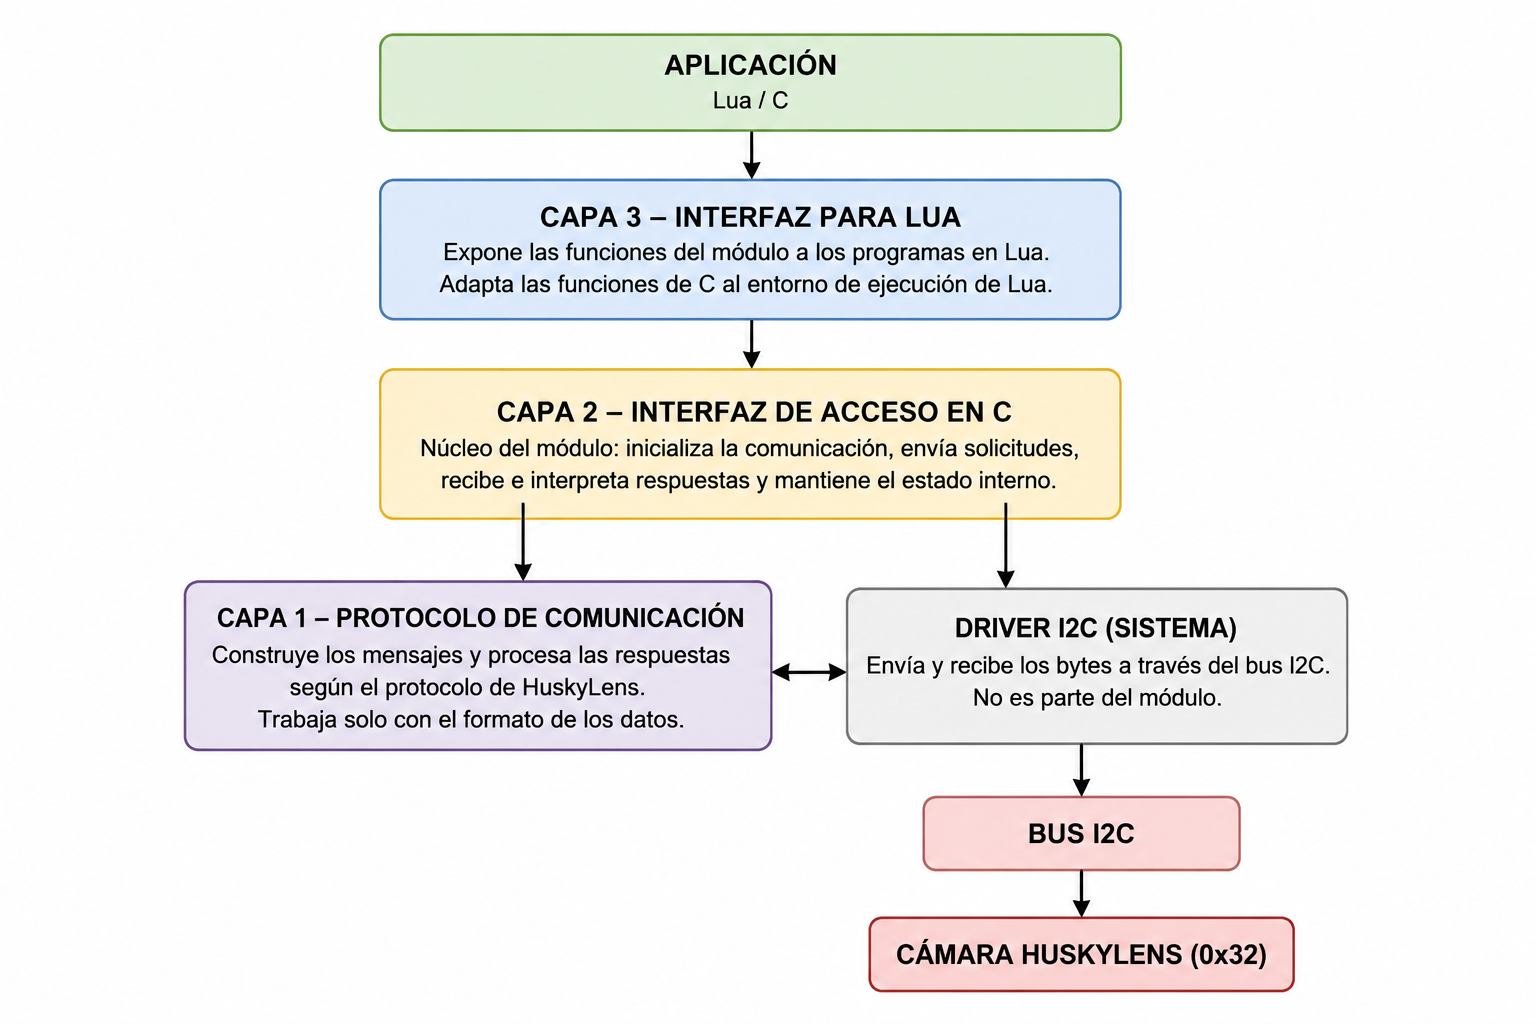
\includegraphics[width=\textwidth]{images/huskylens/modulo_en_capas.png}
    \caption{Arquitectura en capas del módulo de HuskyLens}
    \label{fig:huskylens-modulo-capas}
\end{figure}

% ===== BEHAVIOR TREE =====
\section{Control del comportamiento con Behavior Trees}

Otro de los objetivos es implementar un módulo de \textit{behavior trees} en Lua, con el fin de contar con una alternativa al módulo de máquinas de estado que ya se utiliza en los scripts actuales de Robotito. Con este objetivo en mente, se implementó un módulo completo en Lua que permite desarrollar nuevos scripts para el robot utilizando árboles de comportamiento.

Antes de describir la implementación realizada, se presentan a continuación los fundamentos teóricos de esta arquitectura de control.

\subsection{Fundamentos teóricos}

Los Árboles de Comportamiento (\textit{Behavior Trees}, BT) constituyen una arquitectura de control modular y jerárquica ampliamente utilizada en robótica moderna. Su principal ventaja es la capacidad de organizar comportamientos complejos mediante nodos bien definidos, manteniendo claridad, extensibilidad y una estructura altamente reutilizable.

Un BT se ejecuta mediante \textit{ticks} periódicos. En cada tick se evalúan sus nodos desde la raíz, y cada nodo decide si retorna:

\begin{itemize}
    \item \textbf{SUCCESS}: la tarea asignada se completó correctamente;
    \item \textbf{FAILURE}: la tarea no pudo completarse;
    \item \textbf{RUNNING}: la tarea continúa en progreso y deberá retomarse en ticks futuros.
\end{itemize}

Estos tres estados permiten que el robot reaccione rápido a los cambios del entorno, manteniendo un comportamiento continuo en el tiempo.

\subsubsection{Tipos de nodos}

En la teoría clásica de BT existen tres tipos principales de nodos:

\begin{itemize}
    \item \textbf{Nodos de acción}: encapsulan operaciones concretas. Devuelven SUCCESS si la tarea se completa, FAILURE si es imposible finalizarla, y permanecen en RUNNING mientras la acción está en curso a través de múltiples ciclos.

    \item \textbf{Nodos de condición}: evalúan predicados instantáneos y retornan SUCCESS o FAILURE dependiendo de si la proposición se cumple o no.

    \item \textbf{Nodos compositores}: organizan el flujo del árbol y definen cómo se combinan los nodos hijos. Los dos compositores clásicos son:
    \begin{itemize}
        \item \textit{Sequence}: ejecuta a sus hijos de izquierda a derecha, avanzando al siguiente solo si el anterior devolvió SUCCESS. Si un hijo devuelve FAILURE o RUNNING, el nodo detiene la ejecución y propaga ese estado inmediatamente a su padre.
        \item \textit{Selector} (\textit{Fallback}): diseñado para manejar alternativas o fallos. Intenta ejecutar a sus hijos en orden hasta que uno devuelve SUCCESS o RUNNING, y solo devuelve FAILURE si todos sus hijos fallan.
    \end{itemize}
\end{itemize}

Con estos conceptos como base, se describe a continuación cómo se aplicó esta arquitectura en el módulo desarrollado para Robotito.

\subsection{Arquitectura del módulo BT}

\subsubsection{Rol del BT dentro del sistema}

En la arquitectura del robot, el BT se sitúa como una capa lógica que organiza y ejecuta decisiones de manera ordenada. El motor opera exclusivamente sobre un contexto que contiene el estado del sistema, y los nodos interactúan con funciones de bajo nivel a través de ese contexto. De esta forma, el BT no está atado a un conjunto fijo de acciones, sino que se encarga de coordinar el comportamiento general del robot.

Gracias a esta separación, el BT puede reutilizarse en distintas aplicaciones, no depende del hardware específico del robot, y permite modificar el comportamiento sin necesidad de cambiar su estructura interna. Esto facilita que el proyecto se pueda hacer crecer y mantener de forma ordenada.

\subsubsection{Estructura general del módulo}

El módulo \texttt{bt} implementa únicamente los componentes esenciales para componer comportamientos complejos:

\begin{itemize}
    \item Nodos compositores: \texttt{sequence} y \texttt{selector};
    \item Nodos hoja: \texttt{action} y \texttt{condition};
    \item Decoradores: \texttt{repeater}, \texttt{interrupt}, \texttt{interruptible};
    \item Árbol principal: construido mediante \texttt{bt.create\_tree}.
\end{itemize}

A continuación se describe brevemente cada uno de estos nodos.

\subsection{Implementación de nodos}

El módulo \texttt{bt} desarrollado para este proyecto incluye una colección de nodos diseñada específicamente para funcionar de manera eficiente en Lua-RTOS sobre ESP32. A diferencia de otros motores BT más complejos, esta implementación busca ser simple, consumir poca memoria y evitar referencias circulares.

\begin{itemize}
    \item \texttt{action(fn)}: encapsula una acción potencialmente prolongada, ejecutando la función \texttt{fn(self, ctx)} y retornando SUCCESS, FAILURE o RUNNING según corresponda.

    \item \texttt{condition(fn)}: evalúa una condición instantánea sobre el contexto, retornando SUCCESS o FAILURE sin mantener estado persistente.

    \item \texttt{sequence(children)}: ejecuta a sus hijos en orden y solo avanza al siguiente si el anterior devolvió SUCCESS, deteniéndose y propagando el estado correspondiente ante un FAILURE o RUNNING.

    \item \texttt{selector(children)}: ejecuta a sus hijos en orden buscando la primera alternativa exitosa, deteniéndose ante el primer SUCCESS o RUNNING y devolviendo FAILURE solo si todos sus hijos fallan.

    \item \texttt{repeater(child, n)}: repite la ejecución de su nodo hijo \texttt{n} veces, o indefinidamente si \texttt{n = -1}, reiniciando al hijo entre cada repetición.

    \item \texttt{interrupt(condition, child)}: representa un evento prioritario. Evalúa una condición externa y, si se cumple, ejecuta el nodo hijo asociado a la interrupción.

    \item \texttt{interruptible(child, interrupts, reset\_on\_interrupt)}: envuelve a un nodo hijo principal con una lista de nodos de interrupción, permitiendo abortar su ejecución de forma preventiva si alguno de ellos se activa.

    \item \texttt{create\_tree(root)}: construye la estructura del árbol a partir de un nodo raíz, ejecutando \texttt{root:tick(ctx)} en cada invocación de \texttt{run()}.
\end{itemize}

Este conjunto de nodos conforma un motor BT completo y compacto, adecuado para sistemas embebidos. Mantiene la compatibilidad con las estructuras clásicas de \textit{Behavior Trees} y suma mecanismos de interrupción pensados para entornos reactivos.

A modo de ejemplo, la figura \ref{fig:bt_robotito} muestra el árbol de comportamiento implementado en Robotito, construido a partir de los nodos descritos en esta sección. En él puede observarse cómo los nodos compositores y decoradores se combinan para organizar las distintas tareas del robot en una estructura jerárquica y reactiva.


\begin{landscape}
\begin{figure}[p]
    \centering
    \makebox[\linewidth][c]{%
        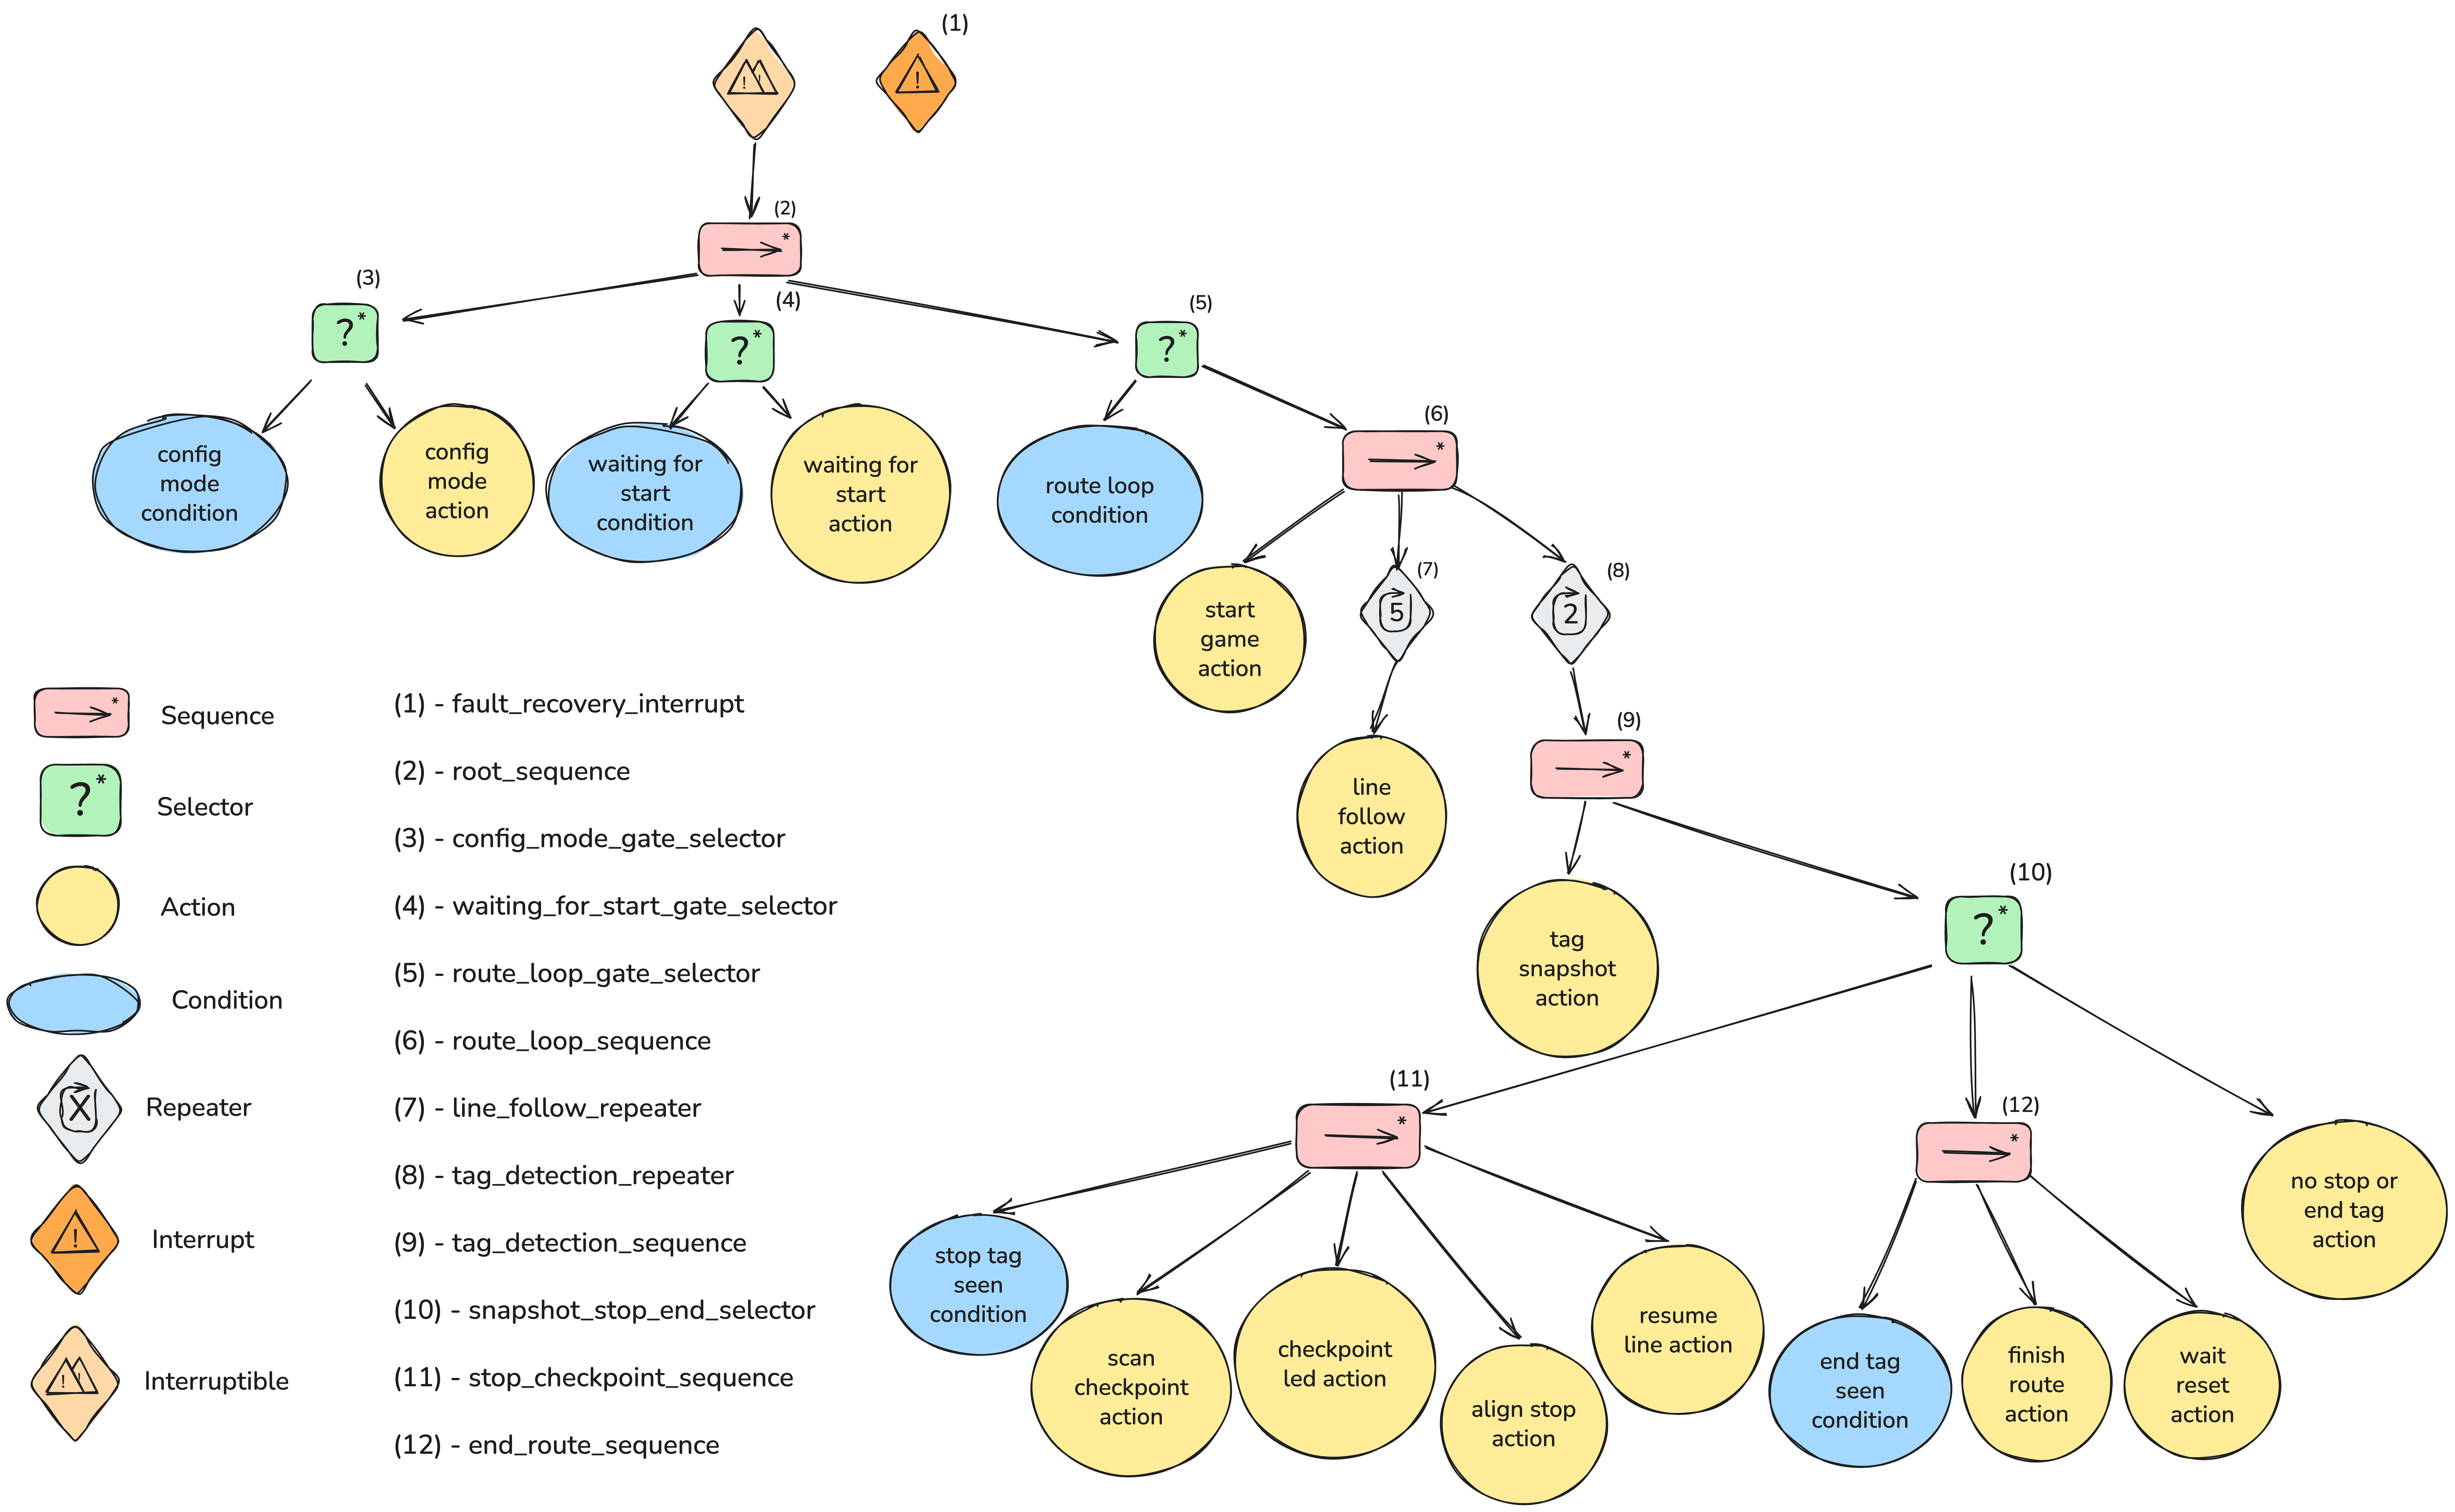
\includegraphics[height=0.92\textheight,keepaspectratio]{images/BTRobotito.png}
    }
    \caption{Árbol de comportamiento implementado en Robotito.}
    \label{fig:bt_robotito}
\end{figure}
\end{landscape}

La implementación del modulo de BT se encuentra en el repositorio  \cite{robotito2026software}.


% ===== WEB =====
\section{Configurador web para la preparación de secuencias}
\label{sec:configurador-web}

Una vez definida la actividad como una secuencia de estaciones identificadas mediante tags, este capítulo presenta la herramienta web utilizada para preparar dicha secuencia antes de transferirla al robot.

\subsection{Rol del configurador web}

Se identificó la necesidad de contar con una herramienta que permitiera preparar recorridos y configuraciones de uso sin modificar directamente el firmware del robot ni depender de entornos de programación complejos. Con este objetivo, se desarrolló un configurador web orientado a facilitar la carga, organización y envío de la secuencia o secuencias de tags a validar por robotito.

Su propósito principal es permitir que el usuario registre tags, defina relaciones de equivalencia entre ellos, construya secuencias de recorrido y valide la configuración antes de su transferencia al robot.

\subsection{Definición de tags y estaciones}

La herramienta permite registrar tags, asociarles nombres o alias y organizarlos según su función dentro de la actividad. De esta forma, el usuario puede trabajar con identificadores comprensibles sin depender únicamente de valores numéricos.

\begin{figure}[!htbp]
    \centering
    \makebox[\textwidth][c]{%
        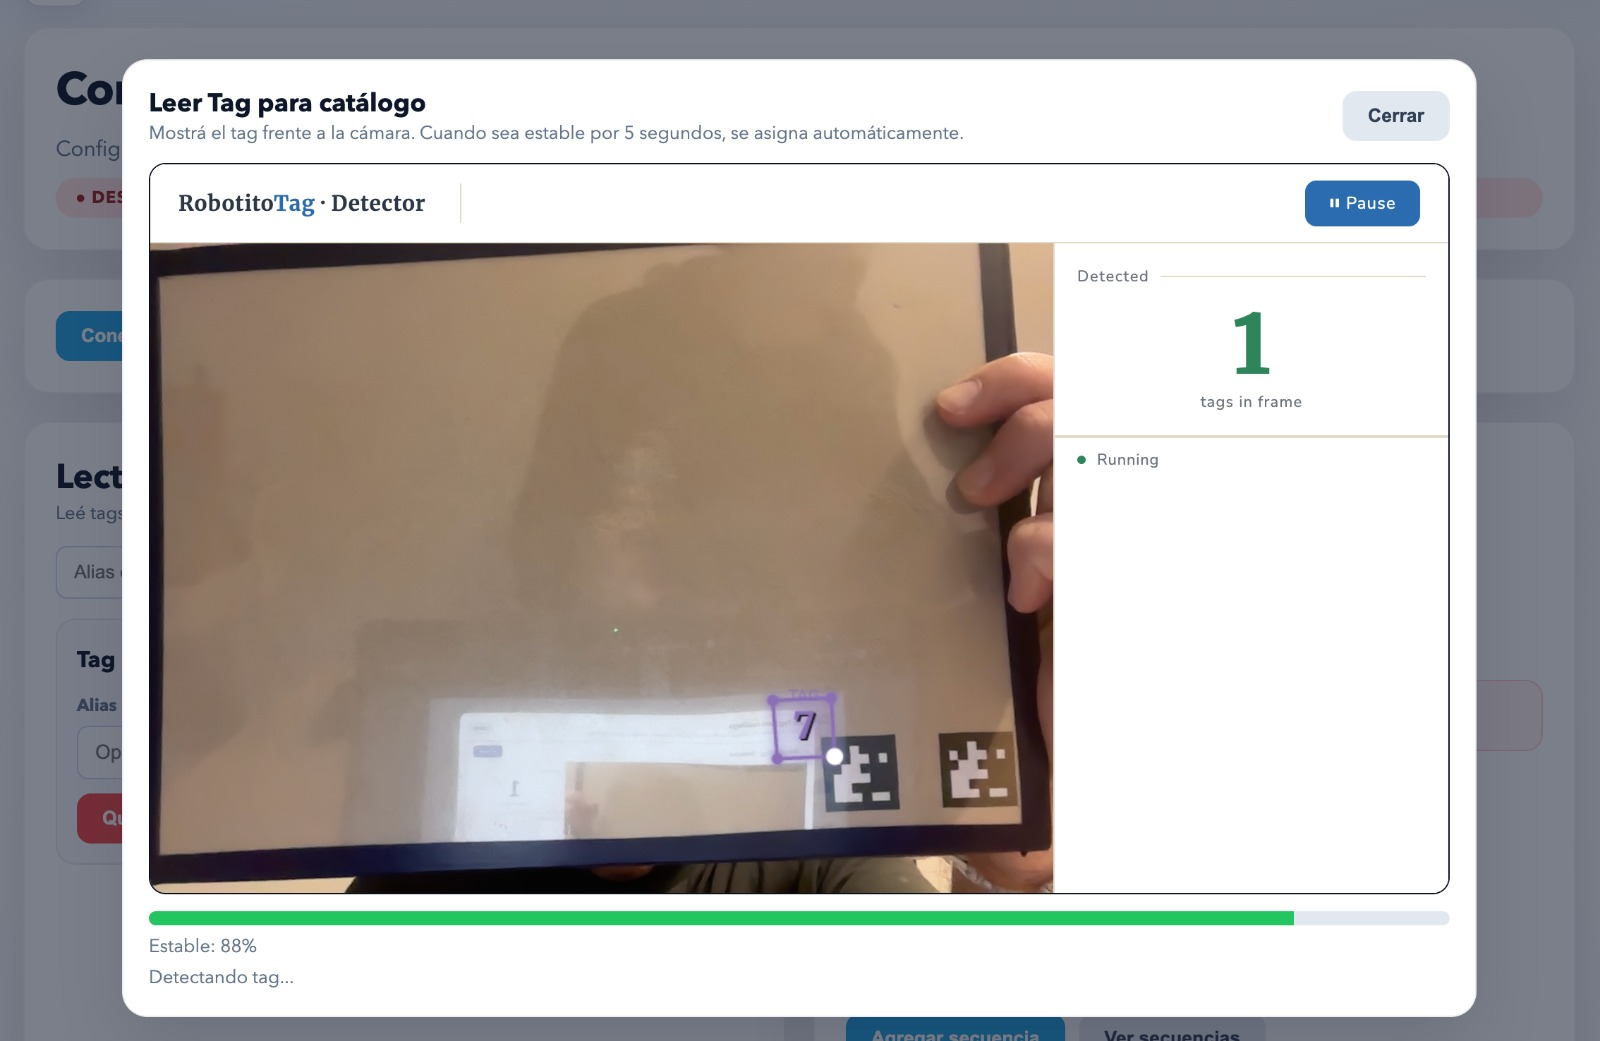
\includegraphics[width=1.3\textwidth]{images/web/tags.jpeg}
    }
    \caption{Lectura de tags.}
    \label{fig:web_tags}
\end{figure}

Además, el configurador incorpora un mecanismo de intercambiabilidad para declarar que distintos tags cumplen la misma función dentro de la actividad. Esto permite que varios tags representen una misma estación cuando la consigna lo requiere.

\subsubsection{Ejemplos de secuencias definidas en el configurador}

Para ilustrar el uso del configurador, se presentan dos ejemplos concretos de secuencias que pueden definirse desde la web.

\begin{enumerate}
    \item \textbf{Secuencia sin intercambiabilidad.} Se define una secuencia de cuatro estaciones con un tag distinto en cada caso:
    \begin{itemize}
        \item Semilla ($T_{1}$)
        \item Planta pequena ($T_{2}$)
        \item Arbol ($T_{3}$)
        \item Arbol con frutas ($T_{4}$)
    \end{itemize}
    En este ejemplo, el robot debe detectar exactamente el orden $T_{1} \rightarrow T_{2} \rightarrow T_{3} \rightarrow T_{4}$.

    \item \textbf{Secuencia con intercambiabilidad.} Se propone formar correctamente la palabra \textit{CASA}. La secuencia objetivo es:
    \begin{center}
        C -- A -- S -- A
    \end{center}
    Las letras A en las posiciones 2 y 4 se modelan con dos tags distintos (por ejemplo, $A_{2}$ y $A_{4}$), pero se declara una relación de intercambiabilidad entre ambos. De esta forma, el sistema acepta cualquiera de esos dos tags en ambas posiciones, manteniendo la validación de la palabra esperada.
\end{enumerate}

\subsection{Construcción y validación de secuencias}

Una vez registrados los tags o cargada una actividad predefinida, el usuario puede construir una o más secuencias de recorrido. Cada secuencia representa el orden esperado de tags que el robot deberá validar durante la actividad.


\begin{figure}[!htbp]
    \centering
    \makebox[\textwidth][c]{%
        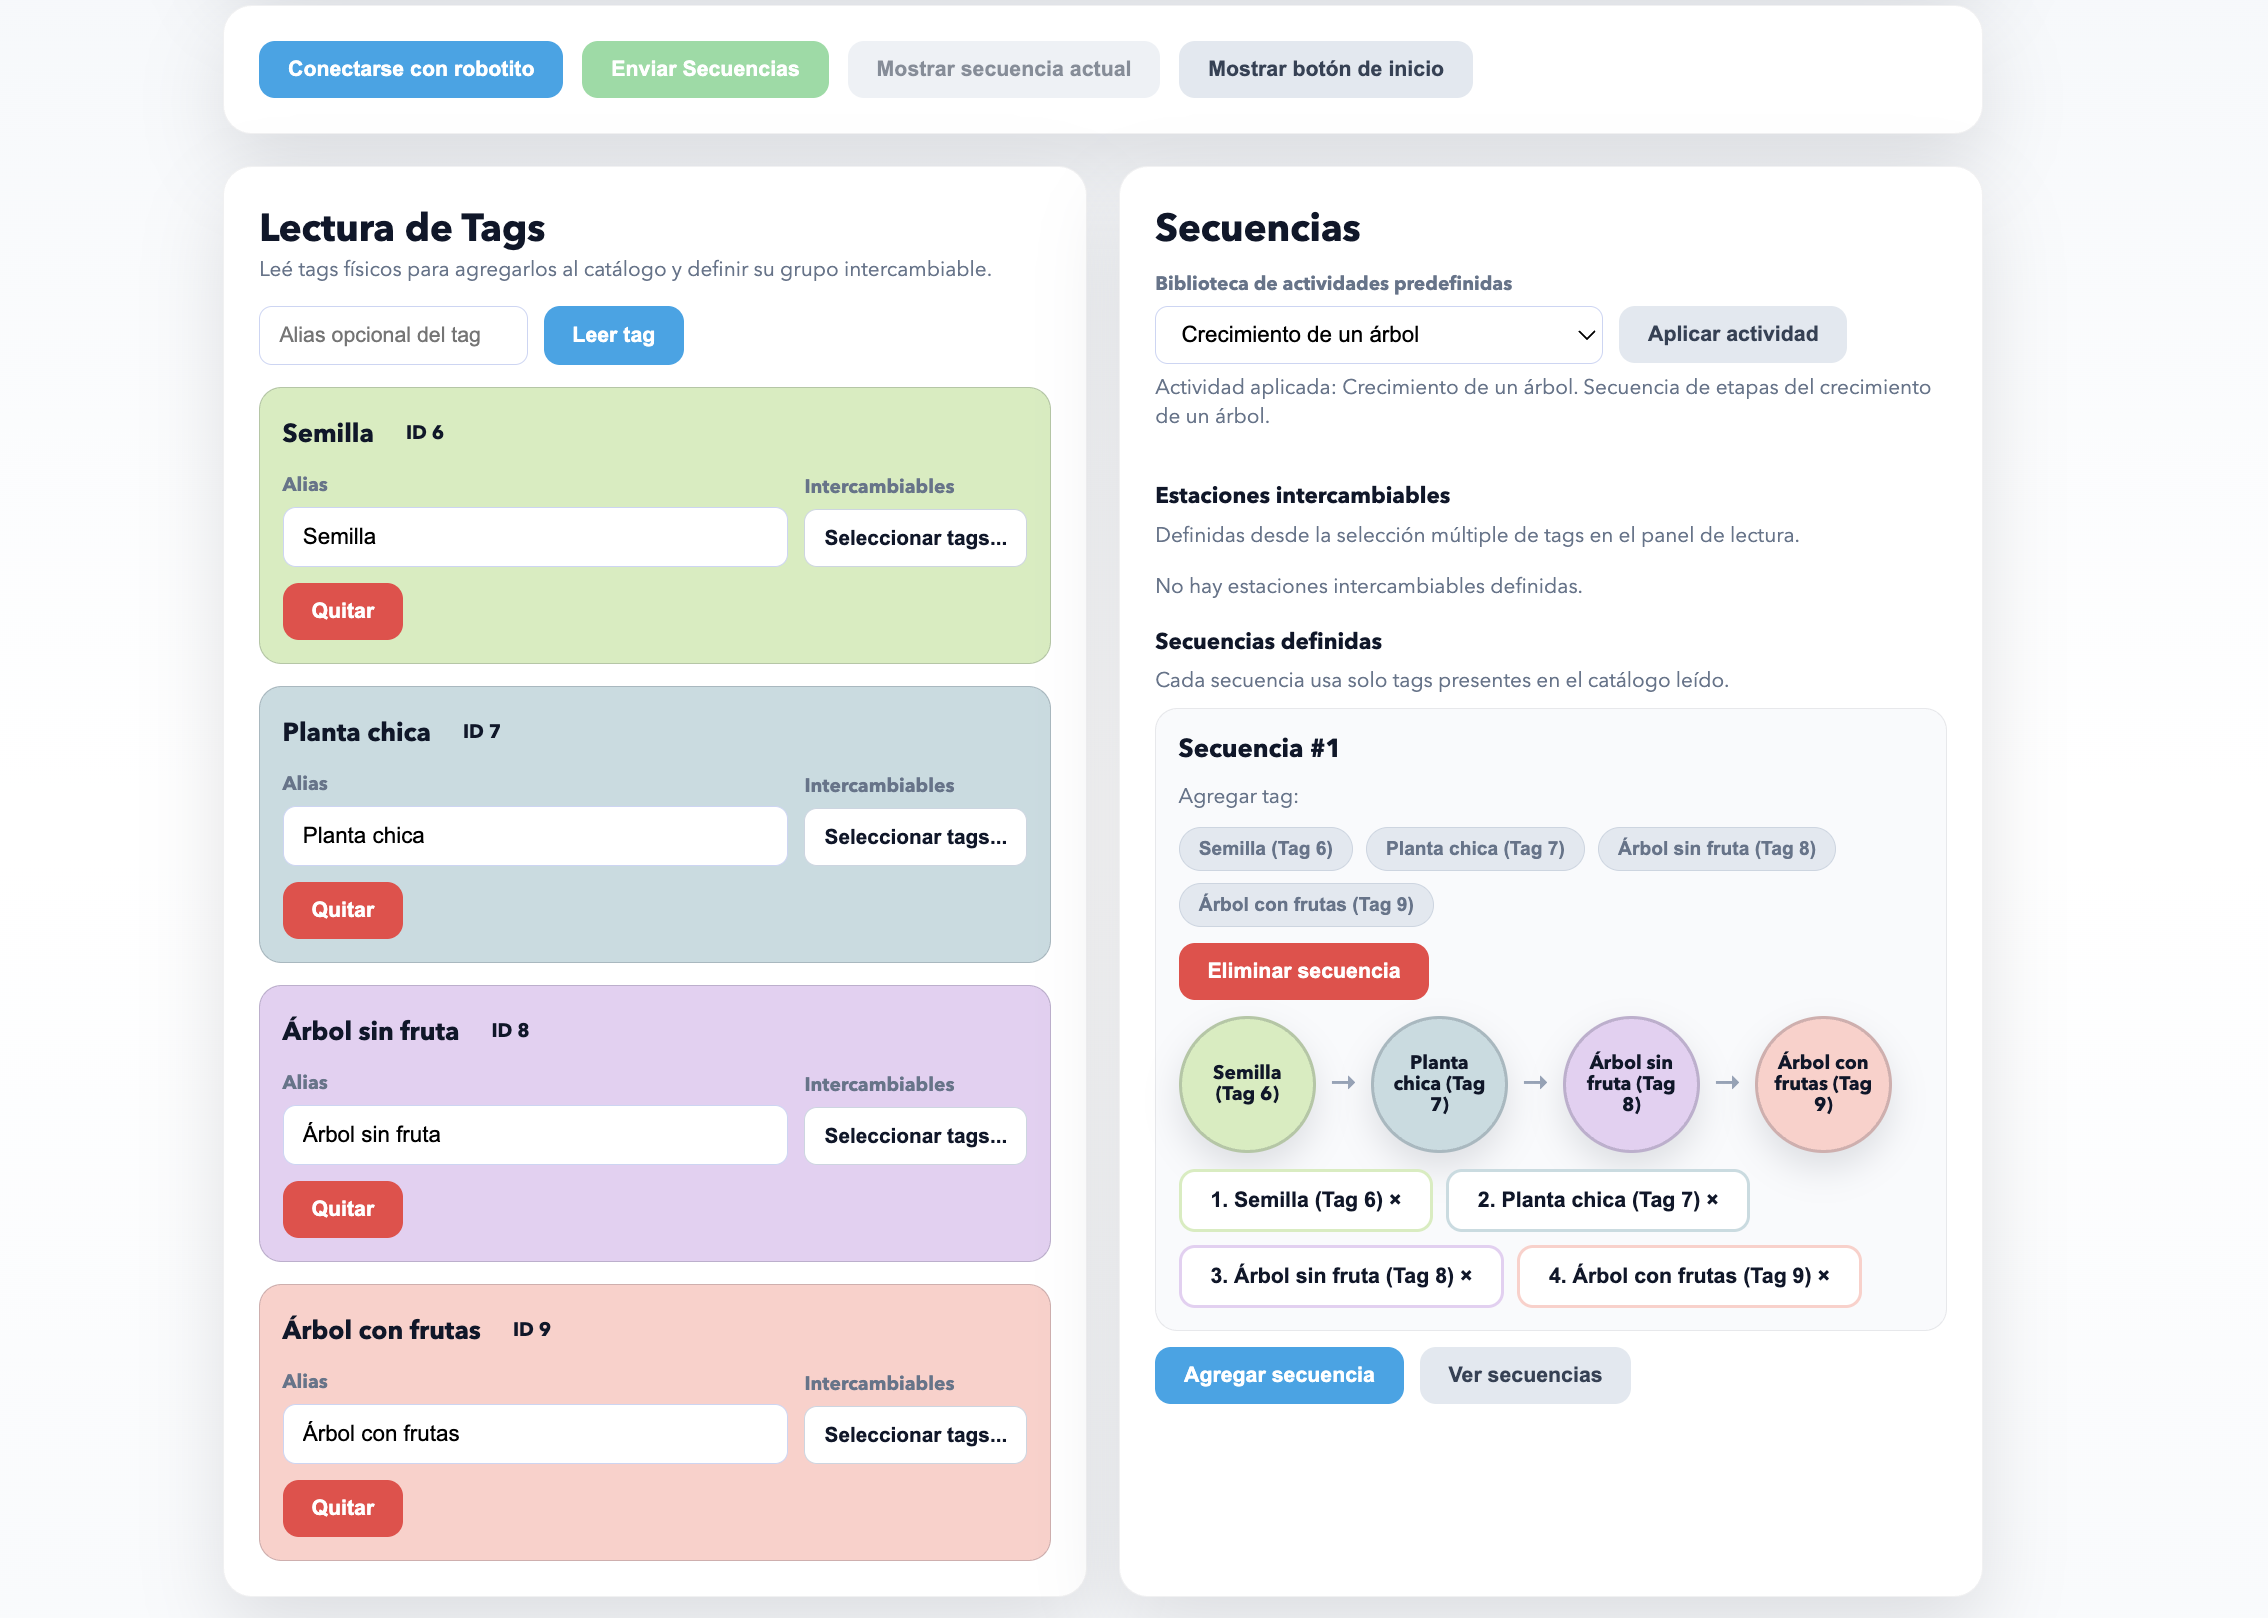
\includegraphics[width=1.3\textwidth]{images/web/secuencias.png}
    }
    \caption{Gestión de secuencias.}
    \label{fig:web_secuencias}
\end{figure}

Antes de enviar la configuración, el sistema verifica que exista al menos una secuencia definida, que no se superen los límites de tamaño de secuencia admitidos y que todos los tags incluidos se encuentren correctamente registrados. Estas validaciones buscan prevenir inconsistencias antes de transferir la información al robot.

\subsection{Biblioteca de actividades y flujo de uso}

El configurador incorpora una biblioteca de actividades predefinidas orientada a reducir el tiempo de preparación. A partir de ella, el usuario puede cargar configuraciones iniciales, ajustarlas según las condiciones del entorno y luego transferirlas al robot.

En términos funcionales, el flujo de uso del configurador es el siguiente:

\begin{enumerate}
    \item El usuario selecciona una actividad predefinida o inicia una configuración manual.
    \item El sistema incorpora los tags, grupos, estaciones y secuencias asociados a la actividad seleccionada.
    \item El usuario registra o ajusta los tags disponibles.
    \item El usuario define, si corresponde, qué tags pueden considerarse equivalentes.
    \item Se construyen o modifican una o más secuencias de recorrido.
    \item El configurador valida que las secuencias sean correctas.
    \item La configuración queda pronta para ser transferida al robot.
\end{enumerate}




%  ===== BLE =====
\section{Configuración de actividades y comunicación BLE}

Luego de construir la configuración de la actividad en la aplicación web, es necesario transferirla al robot. Este capítulo describe la comunicación BLE utilizada para enviar y almacenar esa configuración.

El sistema requiere un mecanismo para transferir al robot la configuración definida por el docente sin modificar el firmware en cada sesión. Este capítulo describe la extensión del canal Bluetooth Low Energy (BLE) utilizada para enviar secuencias, almacenarlas en el robot y exponerlas a la lógica de ejecución.

Para dotar a Robotito de la flexibilidad necesaria en entornos educativos, se ha extendido la funcionalidad del módulo de comunicación \textit{Bluetooth Low Energy} (BLE) original.

\subsection{Gestión de Datos y Persistencia}
La innovación central de la extensión es el \textit{HuskyLens Mapper}, una capa lógica que permite desacoplar los identificadores físicos leídos por la cámara de la lógica semántica de la actividad.

\subsubsection{Almacenamiento No Volátil (NVS)}
Para que el robot sea usable en el aula sin configuraciones repetitivas, el módulo utiliza la memoria flash del ESP32 mediante el sistema \textit{Non-Volatile Storage} (NVS).
El robot restaura automáticamente estos datos al encenderse, permitiendo retomar secuencias previas de forma instantánea. 

\subsection{Arquitectura Multitarea y Sincronización}

Para gestionar el flujo de datos proveniente del Configurador Web sin interferir con la ejecución de los Árboles de Comportamiento, se utiliza un mecanismo de \textbf{Ringbuffer} (buffer circular).
\begin{itemize}
    \item \textbf{Recepción Asíncrona:} Cuando el stack de Bluetooth recibe una trama de configuración, la interrupción de hardware deposita los datos directamente en este buffer.
    \item \textbf{Tarea Dedicada:} Esta tarea de FreeRTOS permanece en estado de espera hasta que el buffer contiene información. Al activarse, extrae los datos y los prepara para la capa de aplicación, garantizando que la llegada de información no bloquee ni ralentice la locomoción o la percepción del robot.
\end{itemize}


\subsection{Integridad de Datos y Mutex}
Dado que el acceso a la memoria compartida donde se almacenan las secuencias puede ocurrir de forma concurrente, se han implementado primitivas de sincronización llamadas \textbf{Mutex}. 

Estos componentes actúan como semáforos de exclusión mutua: si la tarea de Bluetooth está actualizando o cargando datos desde la memoria \textbf{NVS}, el hilo de Lua tiene el acceso bloqueado hasta que la operación finalice. Este mecanismo es crítico para prevenir condiciones de carrera y asegurar que el Árbol de Comportamiento siempre valide la secuencia utilizando información íntegra y consistente.


\subsection{Interfaz con la Capa de Aplicación (API Lua)}
El módulo expone, a través de su API, las funcionalidades necesarias para conectar la lógica de aplicación con el canal de configuración inalámbrica. En la práctica, esta interfaz permite inicializar el stack de Bluetooth y definir el nombre de red visible para el configurador, preparar los mecanismos de sincronización y recuperar desde NVS las secuencias previamente almacenadas, registrar la función de Lua que se dispara automáticamente cuando el docente envía una nueva secuencia desde la web, persistir en memoria flash la lista de objetivos recibida para que el robot conserve la misión aprendida y, finalmente, entregar al Árbol de Comportamiento los identificadores lógicos que deben validarse en cada estación.

Para conocer en profunida la implementación del modulo de BLE, puede visitar el repositorio con su implementación completo \cite{robotito2026hardware}



%%%%%%%%%%%%%%%%%%%%%%%%%%%%%%%%%%%%%%%%%%%%%%%%%%%%%%%%%%%%%%%%%%%%%%%%%%%%%%%%%%%%%%%%%%%%%%%%

% experimentación
\chapter{Experimentación}
\label{cap:experimentacion}

La validación de plataformas educativas requiere no solo verificar su funcionamiento técnico, sino también evaluar su adecuación pedagógica y usabilidad en contextos reales de enseñanza. En este capítulo se describe el proceso de experimentación llevado a cabo para validar la propuesta de extensión de Robotito, tanto desde la perspectiva docente como desde la experiencia directa con estudiantes.
La experimentación se estructuró en dos etapas complementarias: primero, entrevistas semiestructuradas con docentes de nivel inicial y primaria para obtener retroalimentación sobre el diseño de las actividades y la viabilidad práctica de la propuesta; segundo, sesiones presenciales con grupos de estudiantes de educación inicial (entre 4 y 5 años de edad) y educación primaria (entre 7 y 8 años de edad) para observar la interacción directa con el robot y validar los supuestos de diseño.

\section{Metodología}

\subsection{Entrevistas con docentes}

Se realizaron entrevistas semiestructuradas con dos maestras de educación inicial y primaria: Elisa y Cecilia. Ambas docentes cuentan con experiencia en la integración de tecnología en el aula y habían trabajado previamente con robótica educativa en sus instituciones. Si bien no es necesario tener conocimientos tecnológicos o haber realizado algún tipo de actividad similar para poder utilizar Robotito como herramienta de enseñanza, fue beneficioso que sí lo hayan hecho ya que pudieron brindar comentarios útiles en base a experiencias previas que aportaron valor a la versión final del robot y de las actividades definidas.
Las entrevistas tuvieron una duración aproximada de 50 a 60 minutos cada una y siguieron un guión diseñado para abordar los siguientes aspectos:

\begin{enumerate}
\item \textbf{Contexto y materiales físicos}: Evaluación de la propuesta de usar piezas de tatami tipo puzzle para formar la pista del robot, la claridad de los elementos visuales (calles blancas con líneas negras, puntos de parada rojos, similitud con calles y señales de tránsito) y la viabilidad de que los niños armen el circuito de forma autónoma.
\item \textbf{Sistema de tarjetas con tags}: Opinión sobre el uso de etiquetas de tipo \textit{AprilTag} para que el robot pueda leer y validar secuencias, la necesidad de herramientas auxiliares para que los docentes identifiquen el orden correcto de las tarjetas, y estrategias para evitar que los niños memoricen las secuencias según los códigos asociados.
\item \textbf{Retroalimentación del robot}: Tipos de feedback considerados apropiados (visual, sonoro, cinético) ante aciertos y errores, estrategias para manejar la frustración y momento adecuado para entregar la retroalimentación (paso a paso vs. al final del recorrido).
\item \textbf{Dinámica de juego y motivación}: Duración ideal de las actividades, balance entre trabajo colaborativo e individual, tipos de contenido más atractivos (cuentos, palabras, desafíos motrices), y estrategias de cierre.
\item \textbf{Aplicabilidad curricular}: Posibles integraciones con contenidos de diferentes áreas (lenguaje, matemática, ciencias naturales, etc.) y adaptabilidad a distintos niveles educativos.
\item \textbf{Consideraciones prácticas}: Dificultades previstas en términos de tiempo, espacio físico, desarrollo motriz de los niños y nivel de atención esperado.
\end{enumerate}

Las entrevistas se realizaron de forma remota mediante videollamada, con consentimiento explícito de las participantes para el uso de la información obtenida con fines de investigación educativa.

\subsection{Primera sesión práctica con estudiantes}
Posteriormente se organizó una sesión presencial en coordinación con la maestra Cecilia, quien facilitó el acceso a dos grupos de estudiantes de segundo año de educación primaria (niños entre aproximadamente siete y ocho años) con aproximadamente treinta alumnos en total. La actividad se realizó en el salón de clases de la institución educativa.

La sesión se estructuró en etapas progresivas, siguiendo las recomendaciones surgidas de las entrevistas:
\begin{enumerate}
\item \textbf{Discusión previa}: Conversación general sobre la tecnología y la robótica en el día a día.
\item \textbf{Presentación del robot}: Introducción de Robotito y demostración de sus capacidades básicas de movimiento.
\item \textbf{Exploración de materiales}: Manipulación de las piezas de tatami por parte de los estudiantes, observación de las líneas negras y los puntos de parada rojos, e interacción con las tarjetas con tags e imágenes.
\item \textbf{Deducciones}: Etapa de conversación grupal en el que los niños presentan ideas y sugerencias sobre el funcionamiento esperado del robot.
\item \textbf{Construcción del circuito}: En grupos colaborativos, los niños armaron circuitos simples de 3 a 4 puntos de parada.
\item \textbf{Explicación del sistema de validación}: Se presentó el concepto de secuencia correcta y el rol de los tags.
\item \textbf{Ejecución y retroalimentación}: Recorrido del robot por los circuitos armados por los estudiantes, validando las secuencias mediante la lectura de tags y proporcionando retroalimentación inmediata con luces LED (verde para aciertos, rojo para errores).
\item \textbf{Acercamiento final}: Momento de acercamiento por parte de los niños para hacer preguntas y ver el robot de cerca, una vez finalizada la actividad y desarmado el recorrido.
\end{enumerate}

Durante la sesión se realizaron observaciones sistemáticas sobre:
\begin{itemize}
\item Nivel de comprensión de las instrucciones
\item Grado de autonomía en el armado del circuito
\item Capacidad de comprensión del sistema de validación por tags
\item Nivel de atención y motivación sostenida
\item Reacciones emocionales ante aciertos y errores del robot
\item Dinámicas de colaboración entre pares
\end{itemize}

\begin{figure}[!htbp]
    \centering
    \makebox[\textwidth][c]{%
        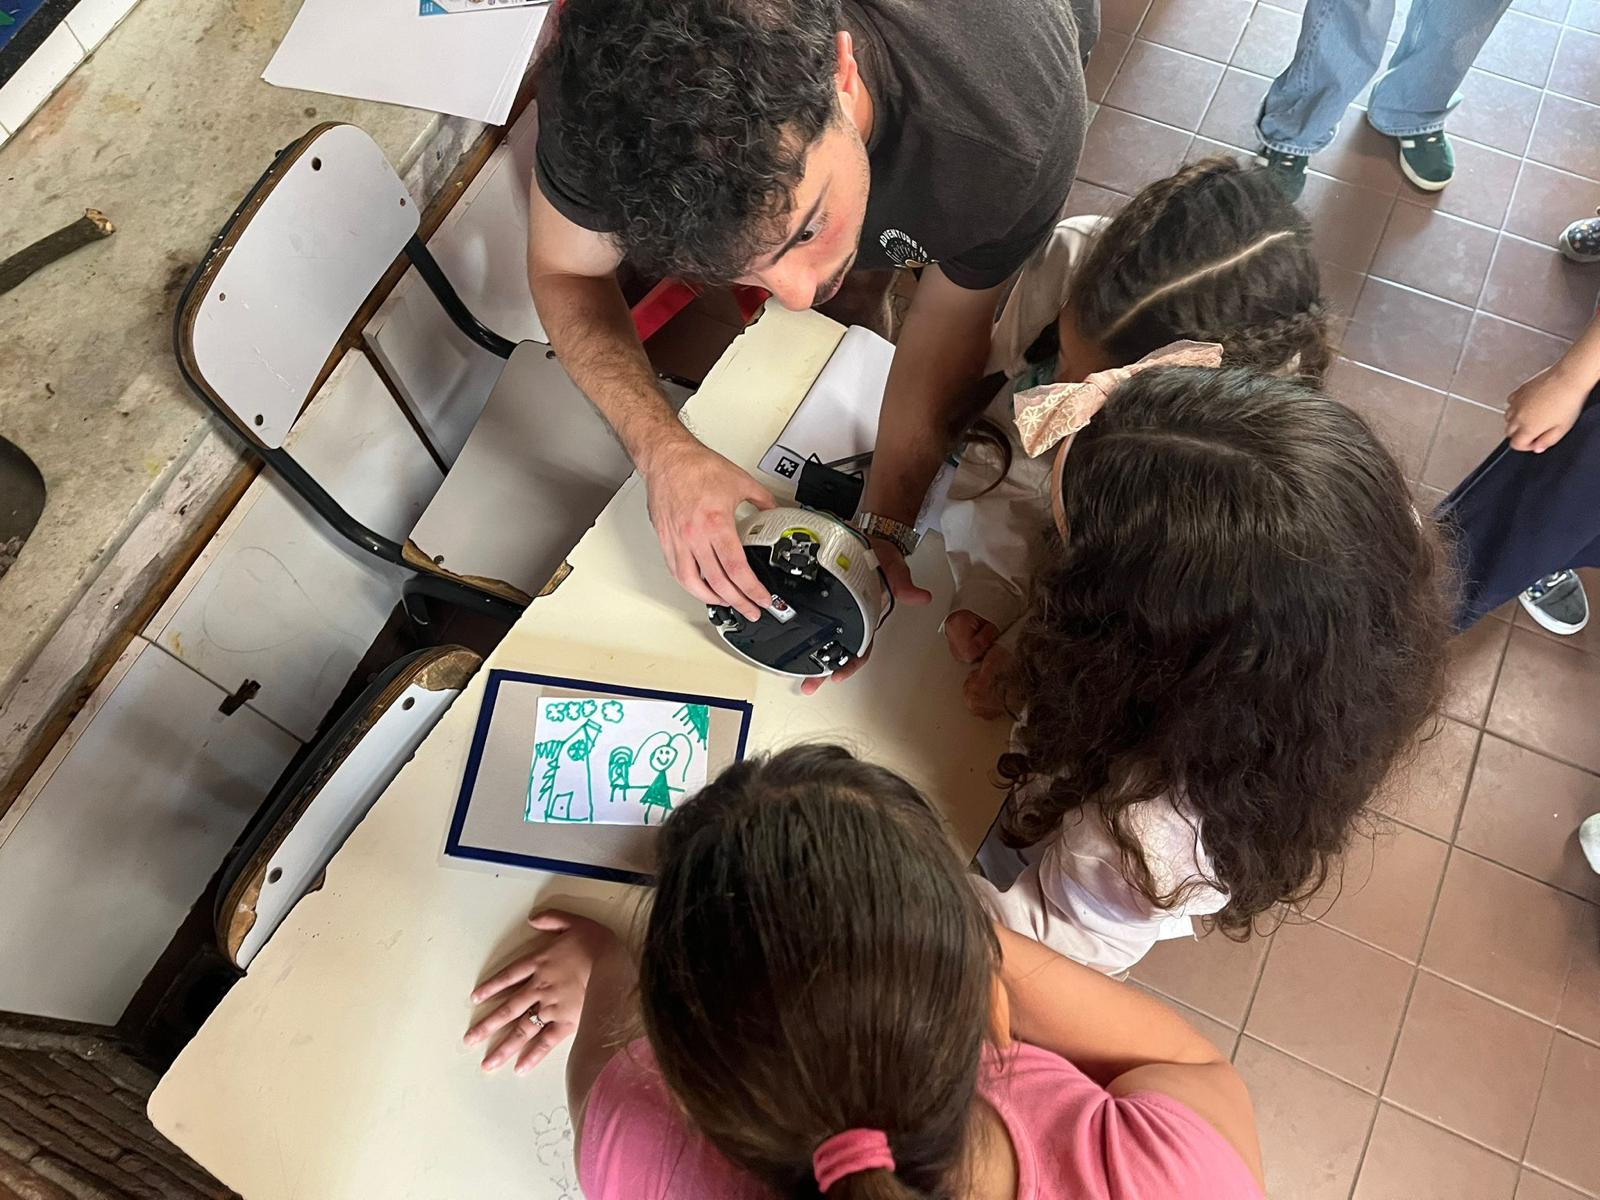
\includegraphics[width=0.9\textwidth]{images/experimentacion/Exp1_1.jpeg}
    }
    \caption{Escuela Nº 168}
    \label{fig:exp_1_1}
\end{figure}

\begin{figure}[!htbp]
    \centering
    \makebox[\textwidth][c]{%
        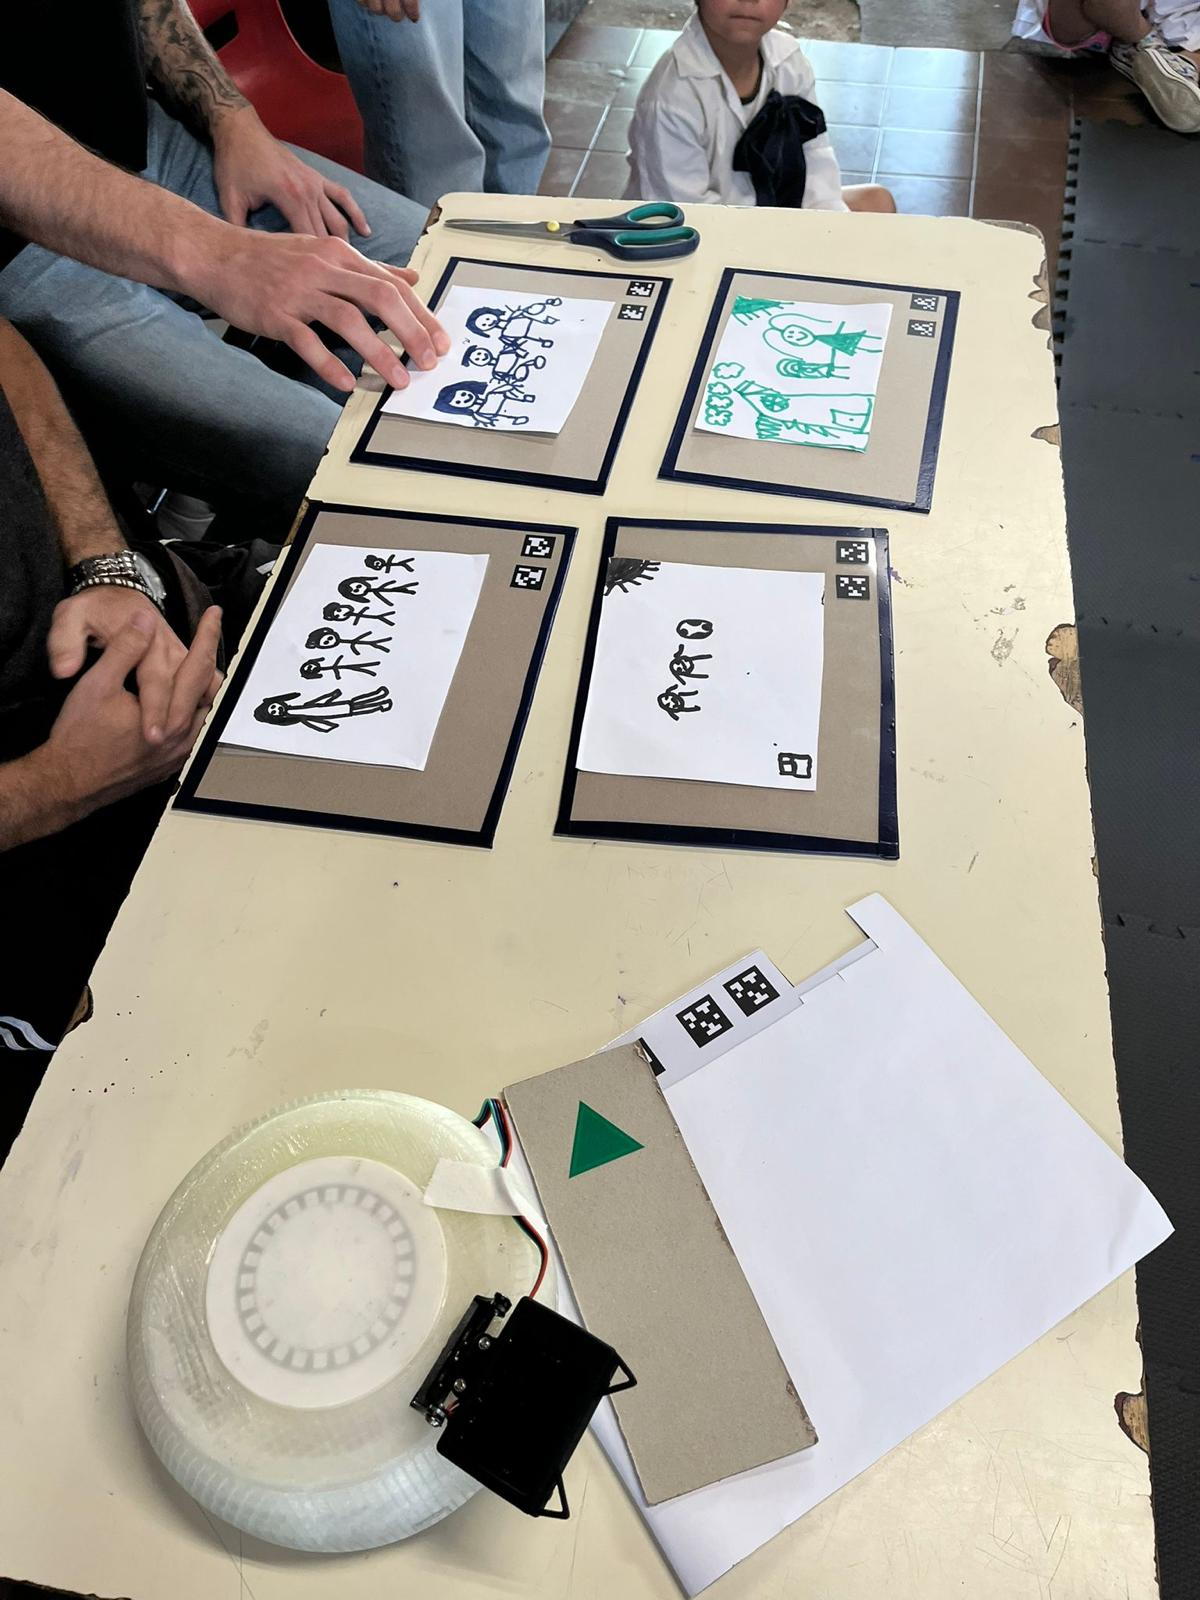
\includegraphics[width=0.9\textwidth]{images/experimentacion/Exp1_2.jpeg}
    }
    \caption{Escuela Nº 168}
    \label{fig:exp_1_2}
\end{figure}

\FloatBarrier

\subsection{Segunda sesión práctica con estudiantes}
En coordinación con la maestra Maria José se organizó otra instancia de actividad práctica, esta vez en otro jardín y con niños de educación inicial (entre cuatro y cinco años). La actividad se realizó en un salón neutro de la institución educativa, esta vez con un grupo reducido de aproximadamente diez alumnos.

La sesión se estructuró en etapas progresivas con algunas diferencias con respecto a la actividad anterior, principalmente debido a la diferencia de edad entre los grupos:
\begin{enumerate}
\item \textbf{Presentación del robot y discusión}: Introducción de Robotito y conversación sobre sus capacidades de movimiento.
\item \textbf{Exploración de materiales}: Manipulación de las piezas de tatami por parte de los estudiantes, observación de las líneas negras y los puntos de parada rojos.
\item \textbf{Construcción del circuito}: Armado de circuitos simples de 3 a 4 puntos de parada.
\item \textbf{Explicación del sistema de validación}: Se presentó el concepto de secuencia correcta y el rol de las tarjetas.
\item \textbf{Ejecución y retroalimentación}: Recorrido del robot por los circuitos armados por los estudiantes, validando las secuencias mediante la lectura de tags y proporcionando retroalimentación inmediata con luces LED (verde para aciertos, rojo para errores).
\item \textbf{Acercamiento final}: Momento de acercamiento por parte de los niños para hacer preguntas y ver el robot de cerca, una vez finalizada la actividad y desarmado el recorrido.
\end{enumerate}

En esta instancia no se pone énfasis en el concepto y utilidad de los tags. Según comentarios de las maestras se decide mejor realizar la actividad teniendo como foco principal el manejo del robot y el concepto de secuencia correcta y secuencia errónea.

\begin{figure}[!htbp]
    \centering
    \makebox[\textwidth][c]{%
        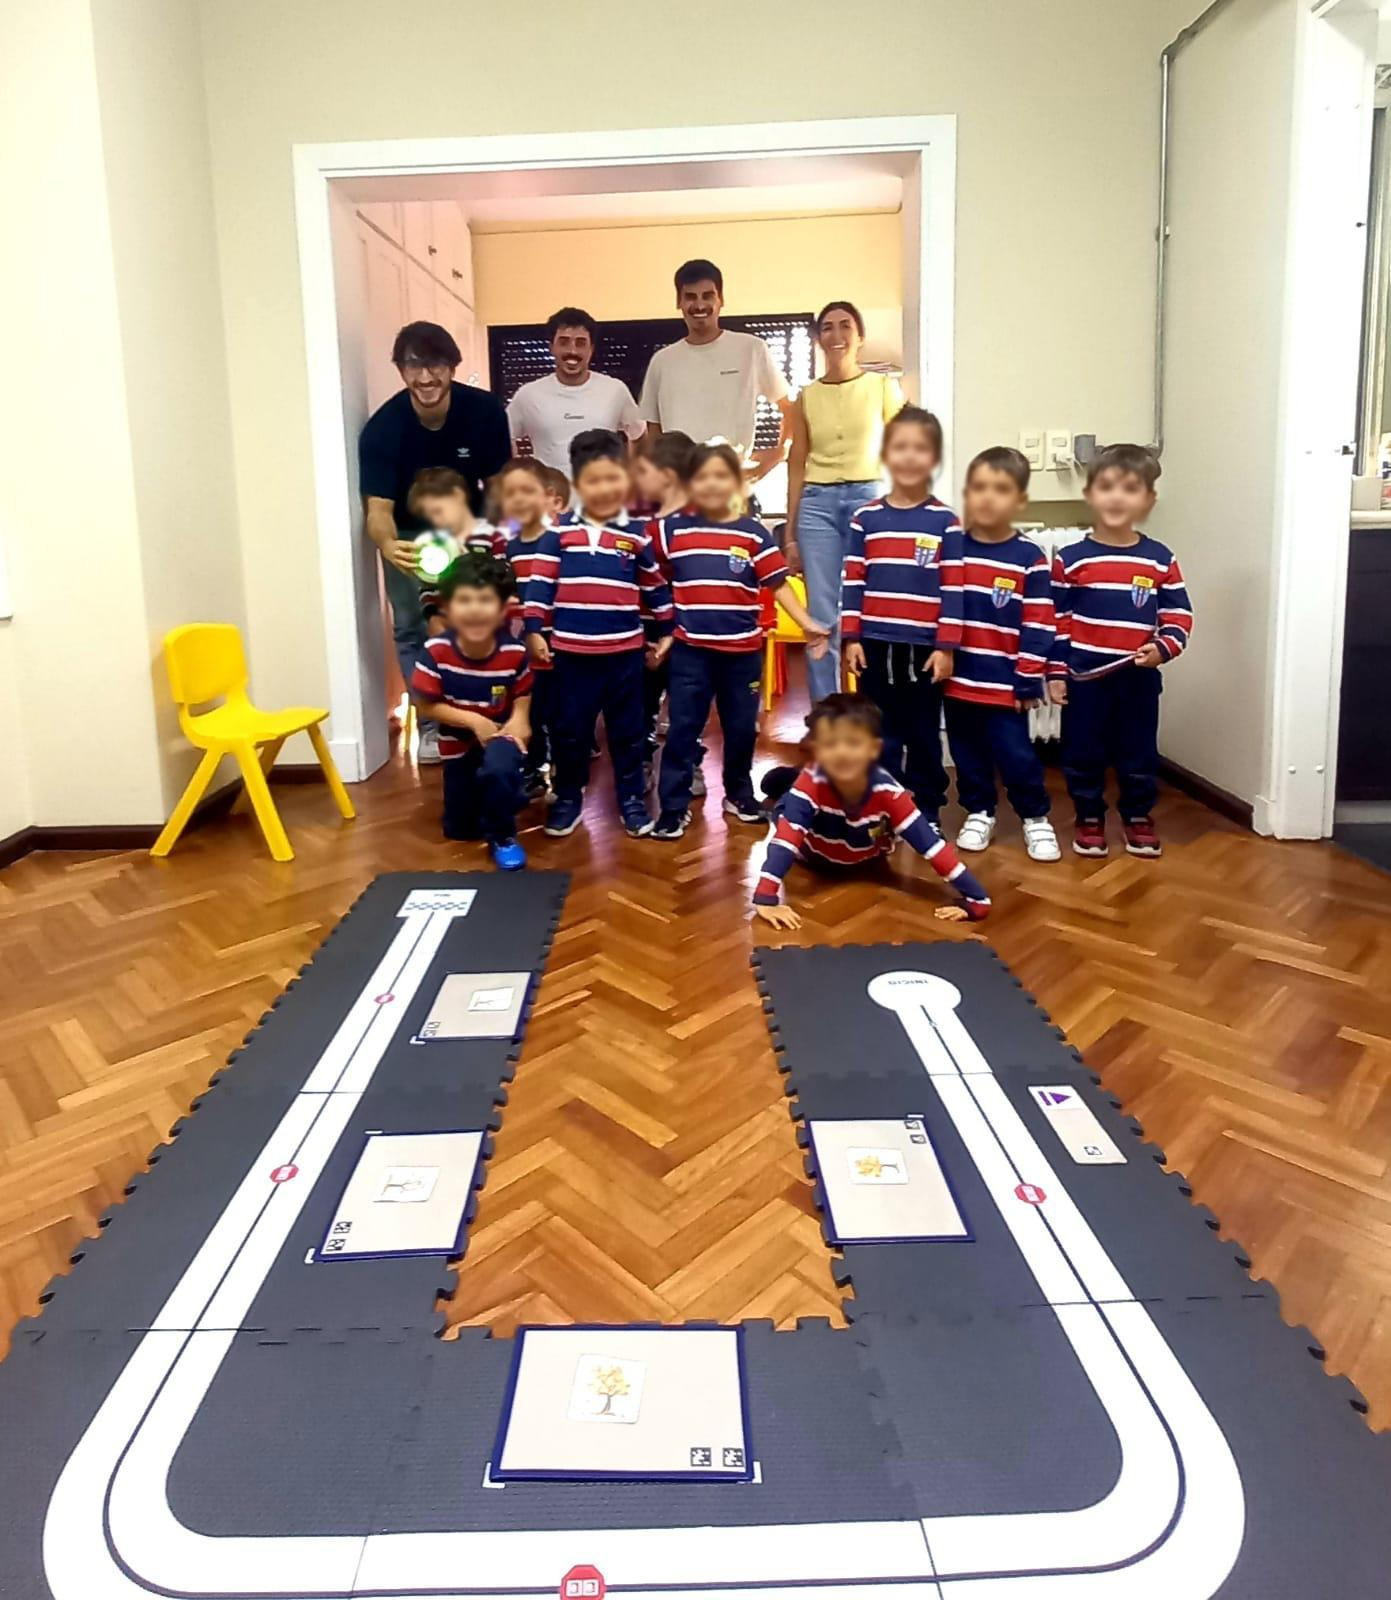
\includegraphics[width=0.9\textwidth]{images/experimentacion/Exp2_1.jpeg}
    }
    \caption{Colegio Richard Anderson}
    \label{fig:exp_2_1}
\end{figure}

\begin{figure}[!htbp]
    \centering
    \makebox[\textwidth][c]{%
        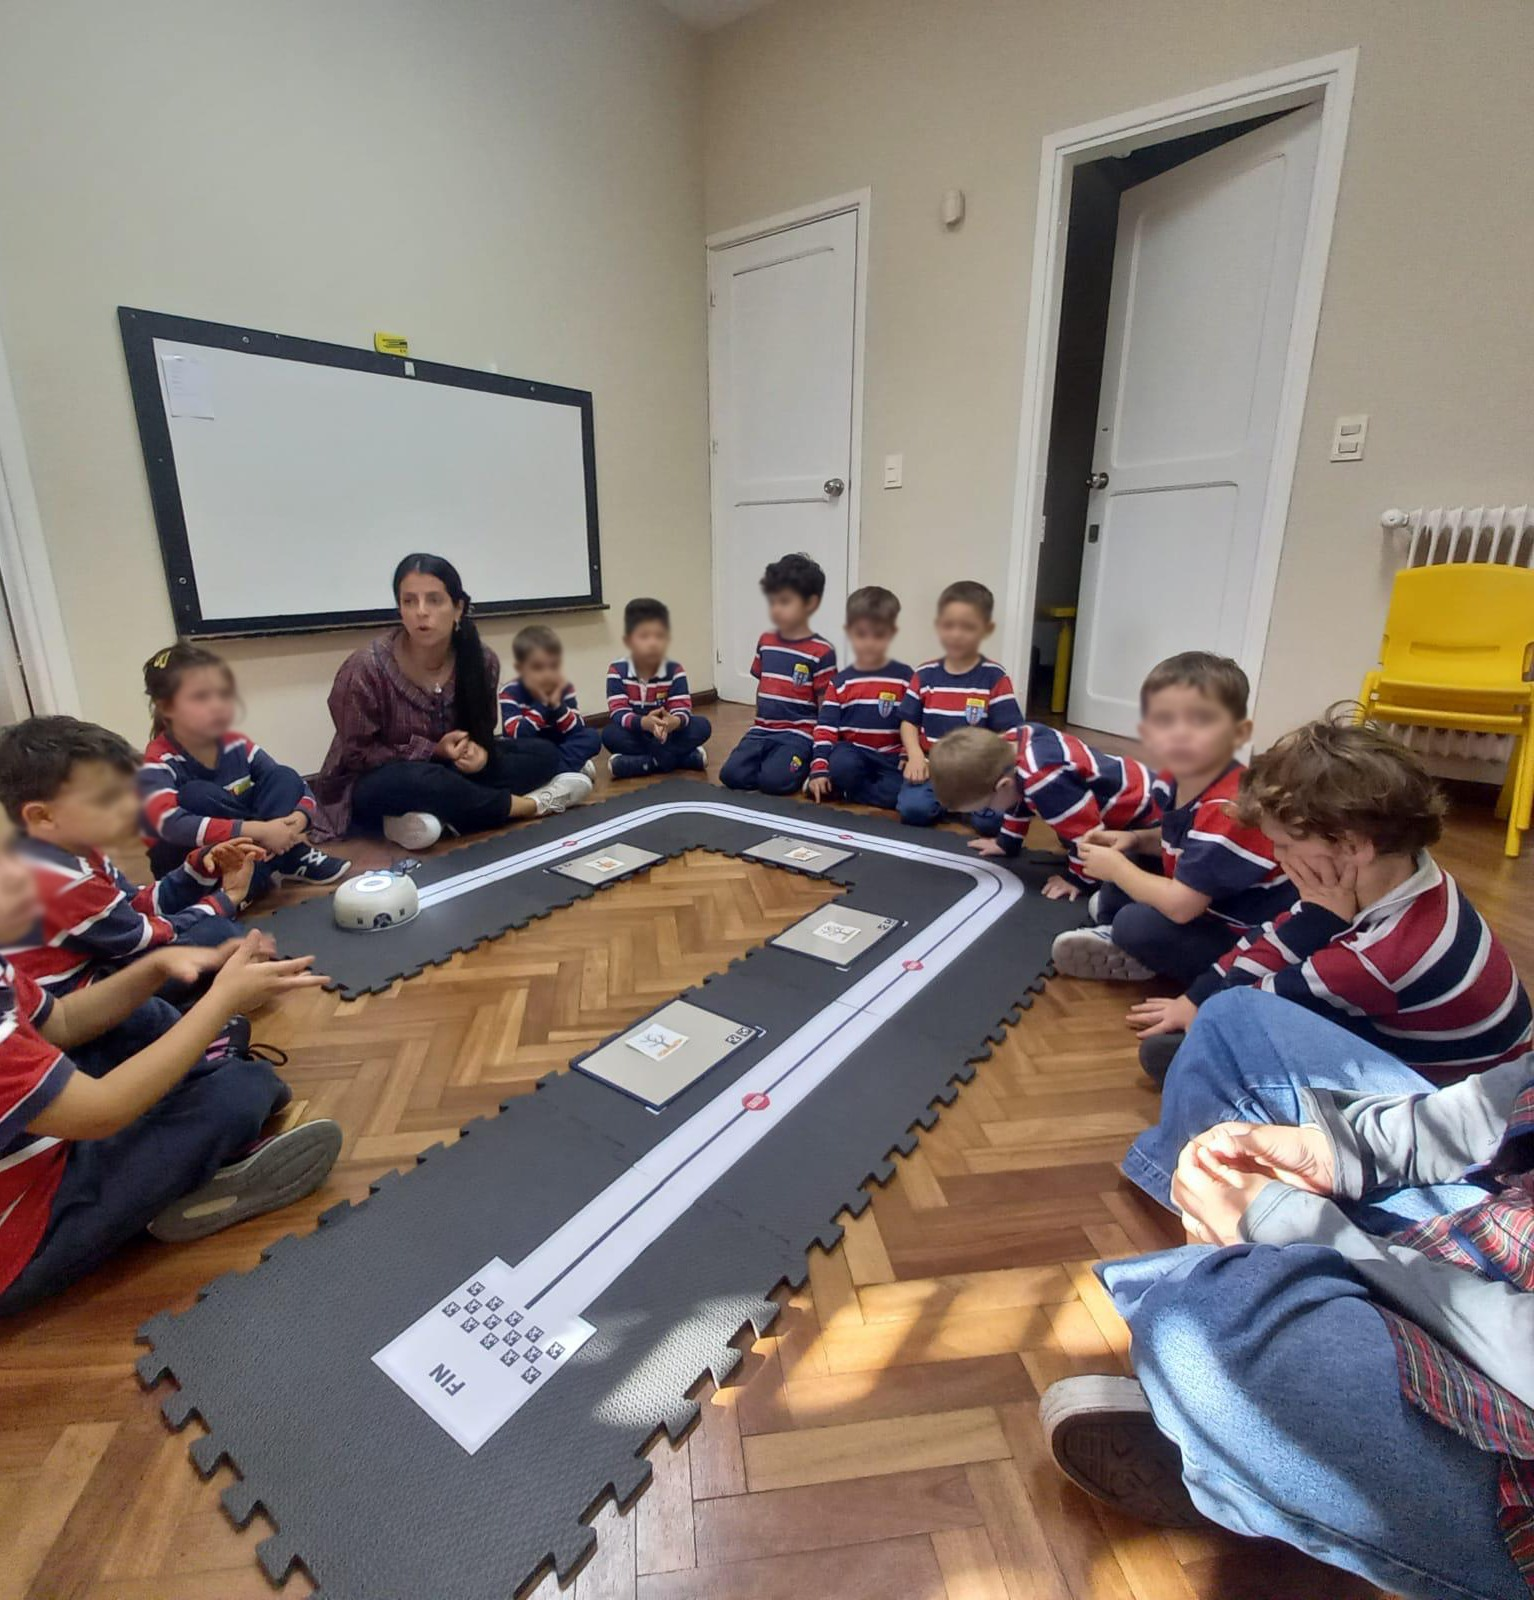
\includegraphics[width=0.9\textwidth]{images/experimentacion/Exp2_2.jpeg}
    }
    \caption{Colegio Richard Anderson}
    \label{fig:exp_2_2}
\end{figure}

\FloatBarrier

\section{Resultados}

\subsection{Retroalimentación de las entrevistas docentes}

Las entrevistas arrojaron comentarios sobre varios aspectos del diseño que se detallan a continuación.

\subsubsection{Diseño de materiales y elementos visuales}
Las docentes validaron positivamente la propuesta de usar piezas de tatami modulares como base física de la actividad. Consideraron que el formato de puzzle es familiar para los niños y facilita tanto el armado colaborativo como la reconfiguración del circuito para diferentes actividades. Sin embargo, sugirieron considerar la durabilidad de los materiales, especialmente de los pegotines de calle con línea negra adheridas, dado el uso intensivo esperado.
Respecto a los puntos de parada, ambas docentes recomendaron reforzar la señal visual del círculo rojo con elementos adicionales que hagan más explícita la acción esperada. Propusieron agregar íconos complementarios como ojos, manos o señales de ``PARE'' que los niños puedan asociar inmediatamente con la acción de detenerse.
\subsubsection{Sistema de tarjetas con tags}
El diseño propuesto de tarjetas---con un tag pequeño para la validación técnica ubicado en una esquina y una imagen central grande para los niños---fue bien recibido. Las maestras destacaron que esta dualidad permite que el contenido educativo sea visualmente predominante, mientras que el aspecto técnico queda en segundo plano.
Elisa y Cecilia plantearon la necesidad de contar con una herramienta auxiliar (aplicación móvil o sistema web) que les permita a los docentes identificar rápidamente qué tag corresponde a cada tarjeta (o qué posición en la secuencia) al momento de preparar las actividades. Sugirieron también implementar un sistema de codificación visual en los bordes de las tarjetas (colores o patrones) que facilite la organización del material sin depender exclusivamente de la tecnología.
Para evitar que los niños memoricen las secuencias por la ubicación física de las tarjetas, propusieron implementar un sistema de rotación de tag, para que en distintas sesiones identifiquen distintos pasos de la secuencia propuesta.
\subsubsection{Progresión pedagógica y etapas diferenciadas}
Una de las recomendaciones más consistentes fue la necesidad de presentar la actividad en etapas claramente diferenciadas, especialmente para niños más pequeños (3 a 5 años). Elisa propuso la siguiente secuencia de complejidad creciente:
\begin{enumerate}
\item \textbf{Etapa inicial}: Introducción al robot y seguimiento libre de líneas sin puntos de parada ni validación.
\item \textbf{Etapa intermedia}: Incorporación de puntos de parada rojos sin validación de secuencia (el robot simplemente se detiene).
\item \textbf{Etapa avanzada}: Introducción del sistema completo con validación de tags y retroalimentación.
\end{enumerate}
Esta progresión permite que los niños comprendan gradualmente cada componente del sistema antes de enfrentarse a la actividad completa.
\subsubsection{Retroalimentación del robot}
Las docentes coincidieron en que la retroalimentación inmediata es fundamental para el aprendizaje, pero debe diseñarse cuidadosamente para no generar frustración excesiva. Recomendaron un sistema de retroalimentación visual mediante luces LED de colores:
\begin{itemize}
\item \textbf{Verde}: Imagen en la posición correcta dentro de la secuencia.
\item \textbf{Rojo}: Imagen en una posición incorrecta dentro de la secuencia.
\end{itemize}
Para el manejo de errores, sugirieron evitar que el robot vuelva automáticamente al inicio tras cada error, ya que esto podría resultar frustrante. En su lugar, propusieron que el robot se detenga en el punto de error, emita la señal visual correspondiente y espere a que los niños corrijan la tarjeta antes de continuar. Esta estrategia mantiene el flujo de la actividad y convierte el error en una oportunidad de reflexión y corrección inmediata.
Al completar exitosamente toda la secuencia, las maestras sugirieron una celebración multimodal: combinación de luces verdes parpadeantes, sonido festivo y, si es posible, algún movimiento expresivo del robot (giro, baile simple).
\subsubsection{Control del flujo de la actividad}
Un aspecto crítico identificado durante las entrevistas fue la necesidad de que los docentes puedan controlar el flujo de ejecución de la actividad. Las maestras plantearon dos situaciones recurrentes en el aula que requerían funcionalidades específicas:
\paragraph{Función de pausa} Los docentes necesitan poder detener el robot en cualquier momento del recorrido para realizar intervenciones pedagógicas oportunas. Situaciones típicas incluyen:
\begin{itemize}
\item Aprovechar un momento de error para generar una discusión grupal sobre la secuencia correcta
\item Atender interrupciones externas (llegada de otro docente, situaciones de convivencia)
\item Permitir que todos los niños del grupo puedan observar un momento específico del recorrido
\item Dar tiempo a los niños para reflexionar sobre lo que el robot hará a continuación
\end{itemize}
\paragraph{Función de reinicio (reset)} La posibilidad de volver a comenzar el recorrido desde cero sin necesidad de apagar y encender el robot resultó fundamental para la dinámica del aula. Esta funcionalidad es necesaria para:
\begin{itemize}
\item Permitir múltiples intentos de la misma secuencia sin interrupciones técnicas
\item Facilitar que diferentes grupos de niños prueben sus propias configuraciones
\item Corregir errores de configuración inicial sin perder tiempo en reinicios manuales
\item Mantener el ritmo de la clase cuando se trabaja con actividades breves y repetitivas
\end{itemize}
Estas sugerencias evidenciaron que el robot no solo debe ejecutar secuencias de manera autónoma, sino también ofrecer puntos de control que permitan al docente mantener la gestión pedagógica de la actividad.
\subsubsection{Aplicaciones curriculares}
Las docentes identificaron múltiples posibilidades de integración curricular. La plataforma permite trabajar con secuencias asociadas a diversas áreas: narrativas de cuentos tradicionales en lenguaje y literatura, procesos naturales como el ciclo de vida de una planta en ciencias naturales, secuencias numéricas y patrones en matemática, o recorridos espaciales que conecten diferentes contextos sociales. Particularmente valoraron la posibilidad de que los niños creen sus propias secuencias mediante dibujos, otorgando mayor sentido de autoría a la actividad.

\subsubsection{Duración y organización de las actividades}
Las maestras recomendaron limitar las secuencias a 3-5 puntos de parada para niños de nivel inicial y primeros años de primaria. Actividades más largas podrían provocar pérdida de atención y dificultad para mantener en mente la secuencia completa.
En cuanto a la duración total de la sesión, sugirieron bloques de 20 a 30 minutos, incluyendo tiempo para el armado colaborativo del circuito, la ejecución y la reflexión posterior. Consideraron fundamental incluir un momento final de cierre donde los niños puedan verbalizar lo que hicieron y aprendieron.
Respecto a la organización, propusieron dinámicas de trabajo en pequeños grupos (3-4 niños) donde se puedan asignar roles rotativos: diseñador del circuito, colocador de tarjetas, observador del robot, y registrador de resultados. Esta distribución de roles fomenta la participación equitativa y el desarrollo de diferentes habilidades.

\subsection{Observaciones de la primera sesión con estudiantes}
La sesión presencial con los dos grupos de segundo año de primaria permitió validar varios de los supuestos de diseño y observar directamente la interacción de los niños con el sistema.
\subsubsection{Comprensión del sistema}
Los estudiantes comprendieron rápidamente el concepto de seguimiento de línea y la función de los puntos de parada rojos. La analogía con las señales de tránsito (semáforo rojo = detenerse) facilitó la comprensión inmediata del sistema.

Un aspecto interesante observado durante la actividad fue la tendencia de los niños a asimilar el robot, o algunas de sus partes, con características humanas. Por ejemplo, varios estudiantes interpretaron la cámara como los ``ojos'' del robot y las ruedas como sus ``piernas''. Estas asociaciones espontáneas facilitaron la construcción de una representación intuitiva del sistema, ya que permitieron vincular componentes técnicos con referencias corporales conocidas por los niños.

Esta forma de interpretación también permitió introducir, de manera implícita, la idea de modularización del robot. Al reconocer que distintas partes cumplen funciones específicas, como ver, moverse o detectar elementos del entorno, se vuelve más comprensible que el robot pueda extender sus capacidades mediante la incorporación de nuevos módulos. En este sentido, la cámara no se percibe únicamente como un accesorio agregado, sino como una funcionalidad adicional que amplía lo que Robotito puede hacer.

Por otro lado, el concepto de secuencia correcta fue inicialmente más abstracto. Algunos niños asumieron que cualquier orden de las tarjetas sería válido. Sin embargo, al presentar ejemplos concretos con narrativas conocidas, la lógica de la secuencia se volvió evidente.

La función de los tags como mecanismo de validación técnica no fue completamente comprendida por todos los niños, pero tampoco resultó necesario que lo comprendieran en profundidad. Para ellos, el robot ``sabía'' si la tarjeta era correcta, lo cual era suficiente para participar en la actividad.
\subsubsection{Autonomía en el armado}
Los estudiantes de segundo año demostraron capacidad para armar circuitos simples de forma relativamente autónoma. Trabajando en grupos de 3-4 niños, lograron conectar las piezas de tatami siguiendo instrucciones básicas. Hubo algunos casos de piezas colocadas en orientaciones incorrectas (línea discontinua, ángulos cerrados), pero con mínima intervención del adulto lograron identificar y corregir los errores.
La colocación de las tarjetas sobre los puntos de parada requirió mayor guía inicial. Algunos niños intentaron colocar múltiples tarjetas en un mismo punto o no alineaban correctamente la tarjeta para que el robot pudiera leer el tag. Tras una demostración y práctica, mejoraron significativamente en esta tarea.
\subsubsection{Motivación y compromiso}
El nivel de motivación fue consistentemente alto durante toda la sesión. Los niños mostraron gran entusiasmo al ver al robot en movimiento y mantuvieron la atención durante las explicaciones cuando estas estaban acompañadas de demostraciones prácticas.

Los niños celebraban espontáneamente cuando el robot completaba exitosamente una secuencia, lo que sugiere que la actividad genera un sentido genuino de logro.
\subsubsection{Reacción ante errores}
Las señales de error (luz roja) no generaron frustración significativa. En la mayoría de los casos, los niños reaccionaron con curiosidad, intentando identificar qué tarjeta estaba en el lugar incorrecto. La recomendación docente de no hacer que el robot vuelva al inicio resultó acertada: permitir que los niños corrigieran el error in situ mantuvo el flujo de la actividad y convirtió el error en una oportunidad de aprendizaje inmediato.
\subsubsection{Colaboración}
Las dinámicas colaborativas funcionaron bien en general. Los niños negociaban espontáneamente quién colocaba cada tarjeta y se ayudaban mutuamente a identificar errores. Sin embargo, en algunos grupos surgieron conflictos menores por el control del material o diferencias de opinión sobre el orden correcto.
La maestra Cecilia intervino en estos casos sugiriendo turnos rotativos y promoviendo el diálogo sobre las razones de cada propuesta, lo que resultó en una experiencia más enriquecedora.

\subsection{Observaciones de la segunda sesión con estudiantes}
La segunda sesión presencial, realizada con un grupo de educación inicial de entre cuatro y cinco años, permitió observar la interacción de niños más pequeños con la plataforma. A diferencia de la primera instancia, el grupo fue reducido, con aproximadamente diez estudiantes, lo que permitió una dinámica más controlada y un acompañamiento más cercano por parte de las maestras.
\subsubsection{Comprensión del sistema}
Debido a la edad de los niños, la comprensión inicial del concepto de robot fue menos precisa que en la primera sesión. Algunos estudiantes asociaron Robotito con una aspiradora robot, utilizando como referencia un objeto tecnológico más familiar en su entorno cotidiano. Si bien estas asociaciones no describían correctamente el propósito del sistema, sí funcionaron como punto de partida para comprender que se trataba de un dispositivo capaz de desplazarse de forma autónoma.

Los niños lograron identificar progresivamente que el robot podía moverse sobre el circuito y detenerse ante ciertas señales. Las señales de parada rojas resultaron especialmente comprensibles, ya que varios estudiantes las relacionaron con la idea de detenerse o esperar. Asimismo, manifestaron curiosidad por la cámara incorporada al robot, realizando preguntas o comentarios sobre su posible función.
\subsubsection{Rol de las docentes durante la actividad}
En esta instancia, la actividad requirió una mediación docente más fuerte que en la sesión anterior. Las maestras guiaron de forma más directa la presentación del robot, el armado del circuito y la interpretación de lo que ocurría durante el recorrido. Esta intervención fue necesaria debido a la edad de los estudiantes y permitió mantener la atención del grupo, ordenar la participación y traducir las consignas a explicaciones más concretas.

A diferencia de la primera sesión, no se generaron instancias extensas de discusión o debate colectivo. Sin embargo, los niños sí participaron mediante comentarios breves, preguntas espontáneas e intentos de anticipar qué debía hacer el robot en cada paso. Esto evidenció que, aunque la actividad debió ser más guiada, seguía habilitando formas iniciales de razonamiento sobre movimiento, secuencia y respuesta del sistema.
\subsubsection{Participación e interés}
La respuesta general de los estudiantes fue muy positiva. Una gran mayoría del grupo se mostró interesada en el robot, observó con atención sus movimientos y participó activamente cuando se les preguntaba qué debía ocurrir a continuación. Varios niños realizaron aportes espontáneos sobre el recorrido, las señales de parada y la función de los elementos visibles del robot.

El tamaño reducido del grupo favoreció que los estudiantes pudieran acercarse, observar el robot con mayor detalle y expresar ideas durante la actividad. Si bien las intervenciones no siempre fueron técnicamente acertadas, sí demostraron curiosidad y disposición a interactuar con la propuesta.
\subsubsection{Adecuación de la actividad para educación inicial}
La sesión permitió comprobar que la propuesta también resulta atractiva para niños de educación inicial, aunque requiere ajustes en la forma de presentación y en el grado de acompañamiento docente. Para este rango etario, la actividad debe apoyarse principalmente en consignas concretas, observación directa del comportamiento del robot y participación guiada en cada etapa del recorrido.

En este sentido, la actividad funcionó adecuadamente cuando fue presentada de forma breve, visual y altamente mediada por las maestras. La experiencia mostró que los niños de cuatro y cinco años pueden comprender qué hace el robot, identificar situaciones simples como el movimiento y la detención ante señales, y participar en la toma de decisiones durante la actividad, aunque todavía no logren formular con precisión qué es un robot o explicar su funcionamiento de manera abstracta.

\section{Análisis, discusión y ajustes}
Los resultados de la experimentación validan la viabilidad tanto técnica como pedagógica de la propuesta. La integración de la cámara HuskyLens con el sistema de tags funciona de manera confiable en condiciones reales de aula, y el diseño de la actividad resulta comprensible y motivador para los estudiantes del rango etario objetivo.

\subsection{Fortalezas identificadas}
\paragraph{Tangibilidad y manipulación física} El uso de materiales físicos (piezas de tatami, tarjetas) favorece el aprendizaje activo y permite que niños con diferentes estilos de aprendizaje se involucren en la actividad. La posibilidad de reconfigurar el circuito otorga un sentido de agencia y creatividad.
\paragraph{Retroalimentación inmediata y visible} El sistema de luces LED proporciona retroalimentación clara, inmediata y no verbal, lo cual es especialmente apropiado para niños pequeños. La retroalimentación visual evita la necesidad de mediación constante del adulto.
\paragraph{Adaptabilidad curricular} La plataforma no está atada a un contenido específico, lo que permite a los docentes integrarla de forma flexible en diferentes áreas y niveles educativos. Esta versatilidad aumenta significativamente su potencial de uso sostenido.
\paragraph{Aprendizaje colaborativo} El diseño natural de la actividad promueve el trabajo en equipo, la negociación y el diálogo, habilidades fundamentales en el desarrollo infantil.
\paragraph{Progresión de complejidad} La posibilidad de utilizar el sistema en diferentes niveles de complejidad (desde seguimiento simple de línea hasta validación completa de secuencias) permite adaptarlo a distintos grupos etarios y niveles de desarrollo.

\subsection{Desafíos y áreas de mejora}
\paragraph{Curva de aprendizaje inicial} Los estudiantes de segundo año de primaria con quienes se realizó la sesión práctica lograron comprender e integrar todos los elementos del sistema (armado del circuito, comprensión de secuencias y validación por tags) dentro de una misma sesión de clase. Sin embargo, para niños de edades más tempranas, es probable que sea necesario planificar sesiones introductorias progresivas que presenten cada componente por separado, tal como sugirieron las docentes entrevistadas.
\paragraph{Gestión de materiales} El sistema requiere múltiples componentes (piezas de tatami, tarjetas, robot) que deben organizarse, almacenarse y mantenerse. Esto puede representar una carga logística para los docentes, especialmente si trabajan con grupos numerosos o tienen limitaciones de espacio físico.
\paragraph{Necesidad de control del flujo de actividad} La experiencia inicial mostró que sin mecanismos de pausa y reinicio, los docentes iban a tener dificultades para gestionar el ritmo de la clase. La imposibilidad de detener el robot para hacer intervenciones pedagógicas o de reiniciar rápidamente para nuevos intentos se determinó como limitante para la flexibilidad de uso en el aula. Este feedback fue determinante para la incorporación de los controles de flujo mencionados.
\paragraph{Dependencia de elementos técnicos} Aunque el sistema es robusto, depende del correcto funcionamiento de la cámara y de la lectura de tags. En la primera sesión con estudiantes se observó una falla de lectura asociada a las condiciones de iluminación del salón, dado que en ese momento el robot utilizaba reconocimiento de colores para identificar las zonas de parada. Esta situación motivó un ajuste en el funcionamiento del sistema: las acciones del recorrido dejaron de depender de la detección de colores y pasaron a ser activadas mediante la lectura de tags. A partir de este cambio, la lógica principal de la actividad quedó basada en el seguimiento de líneas y el reconocimiento de tags, reduciendo la dependencia respecto a la iluminación ambiente para la detección de los puntos de parada. De todos modos, tags dañados, mal alineados o mal ubicados pueden interrumpir la actividad, por lo que es importante desarrollar protocolos para el mantenimiento y la resolución rápida de este tipo de problemas.
\paragraph{Necesidad de herramientas auxiliares para docentes} La solicitud de una herramienta que permita a los docentes identificar tags mediante sus teléfonos móviles es legítima y necesaria. Sin esta herramienta, la preparación de actividades se vuelve más compleja y propensa a errores.
\paragraph{Riesgo de memorización} Sin un sistema de rotación de tags, los niños podrían memorizar posiciones físicas en lugar de razonar sobre secuencias lógicas. Esto disminuiría el valor educativo de la actividad.

\subsection{Validación de decisiones de diseño}
La experimentación validó varias decisiones de diseño tomadas durante el desarrollo:
\begin{enumerate}
\item \textbf{Uso de HuskyLens sobre otras cámaras}: La capacidad de reconocimiento confiable de tags en tiempo real demostró ser adecuada para el contexto educativo. La alternativa de procesamiento remoto habría agregado complejidad innecesaria.
\item \textbf{Eliminación del reconocimiento de colores en puntos de parada}: La primera instancia con estudiantes permitió identificar que la detección de colores podía verse afectada por las condiciones de iluminación del salón. A partir de esta observación, se decidió que las acciones del recorrido no fueran activadas por reconocimiento de colores, sino mediante la lectura de tags. Esta modificación fue validada en la segunda instancia, donde no se observaron problemas de lectura asociados a la iluminación de la sala.
\item \textbf{Retroalimentación paso a paso vs. final}: La retroalimentación inmediata en cada punto de parada resultó más efectiva pedagógicamente que esperar al final del recorrido \cite{marwan2022adaptiveFeedback}.  Permite correcciones oportunas y mantiene el foco de los niños.
\item \textbf{Sistema modular de piezas de tatami}: El formato de puzzle resultó intuitivo y práctico. La modularidad permite escalabilidad (circuitos más largos o complejos) sin requerir nuevos materiales fundamentalmente diferentes.
\item \textbf{Integración de árboles de comportamiento}: Aunque no fue visible para los usuarios finales, la arquitectura basada en Behavior Trees facilitó la implementación de la lógica de control y permitirá futuras extensiones del comportamiento del robot de forma ordenada y mantenible.
\end{enumerate}

\subsection{Ajustes realizados basados en el feedback}
Como resultado de la experimentación, se implementaron y planificaron diversos ajustes:

\paragraph{Mejoras en señales visuales de parada} Se reforzaron los círculos rojos con iconografía adicional (señal de ``PARE'' estilizada) para hacerlos más explícitos, especialmente para niños más pequeños.
\paragraph{Calibración de retroalimentación luminosa} Se ajustó la intensidad y duración de las señales LED para que sean claramente visibles incluso en ambientes bien iluminados, pero sin resultar abrumadoras. Se define además que previo a realizar la retroalimentación luminosa el robot debe mostrarse en un estado ``pensativo'' (sin movimiento, con las luces LED ``girando'' por un segundo) para darle tiempo a los niños que entiendan exactamente qué está pasando en cada paso del recorrido.
\paragraph{Implementación de controles de flujo} En respuesta directa al feedback docente, se incorporaron dos funcionalidades esenciales:
\begin{enumerate}
\item \textbf{Función de pausa}: Se implementó un mecanismo que permite al docente detener la ejecución en cualquier momento realizando la acción de levantar el robot. Cuando se activa la pausa:
\begin{itemize}
\item El robot detiene su movimiento inmediatamente y se activa el modo ``pausa''
\item Se mantiene el contexto de la actividad (no pierde el progreso)
\item Puede reanudarse desde el mismo punto al reubicarlo en el recorrido y mostrar el tag correspondiente a ``iniciar''
\item Permite intervenciones pedagógicas sin interrumpir el flujo lógico de la secuencia
\end{itemize}
\item \textbf{Función de reset}: Se agregó una etiqueta específica (tag) que permite reiniciar el recorrido y comenzarlo desde cero. Esta función:
\begin{itemize}
\item Reinicia el estado interno del robot (contador de secuencia, validaciones previas)
\item Posiciona virtualmente al robot al inicio del circuito
\item Limpia los registros de aciertos/errores anteriores
\item Permite comenzar una nueva ejecución rápidamente sin manipulación física del robot
\end{itemize}
\end{enumerate}
Ambas funcionalidades se diseñaron para ser accesibles en base a acciones simples, permitiendo que los docentes mantengan el control pedagógico de la actividad en tiempo real sin depender de conocimientos técnicos avanzados.
\paragraph{Documentación de progresión pedagógica} Se elaboró material de guía para docentes que describe explícitamente las tres etapas de complejidad creciente (seguimiento libre, paradas simples, validación completa) con ejemplos de actividades para cada nivel, incluyendo ahora recomendaciones sobre cuándo y cómo utilizar las funciones de pausa y reset.

\section{Conclusiones del proceso de experimentación}
La experimentación realizada demuestra que la extensión de Robotito con capacidades de visión artificial y validación de secuencias es técnicamente funcional y pedagógicamente valiosa. La plataforma logra integrar pensamiento computacional, razonamiento secuencial y contenidos curriculares diversos en una experiencia de aprendizaje tangible y motivadora.
El proceso iterativo de diseño, desde las entrevistas con docentes expertas hasta la validación práctica con estudiantes, resultó fundamental para identificar y resolver aspectos que no habrían sido evidentes desde una perspectiva puramente técnica. Las recomendaciones de las maestras sobre progresión pedagógica, gestión de la frustración y adaptabilidad curricular enriquecieron significativamente el diseño final.
Las sesiones con estudiantes confirmaron que la propuesta es accesible y atractiva para el público objetivo, aunque también evidenció la necesidad de herramientas de apoyo para los docentes y protocolos claros para el uso efectivo del sistema. En particular, la incorporación de las funciones de pausa y reset surgió como un elemento crítico para permitir que los docentes mantengan el control pedagógico de la actividad sin sacrificar la autonomía del robot.
En conjunto, la experimentación valida que Robotito extendido con visión artificial constituye una herramienta educativa viable que puede contribuir al desarrollo del pensamiento computacional y al aprendizaje de contenidos curriculares en edades tempranas, cumpliendo así con los objetivos educativos planteados en este proyecto.

%%%%%%%%%%%%%%%%%%%%%%%%%%%%%%%%%%%%%%%%%%%%%%%%%%%%%%%%%%%%%%%%%%%%%%%%%%%%%%%%%%%%%%%%%%%%%%%%


%%%%%%%%%%%%%%%%%%%%%%%%%%%%%%%%%%%%%%%%%%%%%%%%%%%%%%%%%%%%%%%%%%%%%%%%%%%%%%%%%%%%%%%%%%%%%%%%

%conclusiones
\chapter{Conclusiones y Trabajo Futuro}
\label{cap:conclusiones}
\section{Conclusiones}

Este trabajo aporta una extensión concreta y acotada de la plataforma educativa Robotito, desarrollada sobre cuatro frentes: percepción visual limitada al seguimiento de línea y a la lectura de tags mediante la cámara HuskyLens, configuración inalámbrica de actividades mediante un configurador web y un módulo de comunicación Bluetooth con persistencia en NVS, control modular del comportamiento del robot mediante Árboles de Comportamiento e integración de estas tres piezas en una actividad educativa concreta, puesta a prueba en dos instancias con estudiantes de entre 4 y 8 años.

Desde el punto de vista técnico, se desarrollaron tres componentes reutilizables e independientes entre sí, que en conjunto sostienen estos cuatro frentes. El módulo HuskyLens abstrae la complejidad del protocolo de comunicación con la cámara, exponiendo una interfaz uniforme accesible desde C y desde Lua, acotada a las dos capacidades utilizadas en este trabajo: seguimiento de línea y lectura de tags. El motor de Árboles de Comportamiento provee una biblioteca de control general, desacoplada de cualquier lógica de dominio específica, que permite modelar nuevos comportamientos robóticos combinando los nodos existentes sin modificar el núcleo del sistema. La extensión del módulo Bluetooth, junto con el configurador web, resuelve la configuración inalámbrica de actividades: permite preparar una secuencia desde una aplicación externa y transferirla al robot sin modificar su firmware, con persistencia entre sesiones. La integración de estos tres componentes en la actividad implementada muestra que la arquitectura funciona de forma coordinada en un escenario similar al de una clase real, y es la instancia donde efectivamente se validó el aporte del proyecto.

Un resultado adicional del proceso de desarrollo fue la importancia de iterar sobre decisiones técnicas a partir de la puesta a prueba con usuarios reales, dentro de ese mismo frente de integración: la primera sesión con estudiantes evidenció que la detección de puntos de parada basada en reconocimiento de colores era sensible a las condiciones de iluminación del aula, lo que llevó a rediseñar esa lógica para depender exclusivamente de la lectura de tags. Este cambio fue validado en la segunda sesión, donde no se observaron problemas de lectura asociados a la iluminación, y confirma que someter la solución a condiciones de uso reales permitió detectar y corregir un problema que no era evidente desde un análisis puramente técnico.

Desde el punto de vista pedagógico, la experimentación con tres maestras de nivel inicial y primaria y dos sesiones con estudiantes de entre 4 y 8 años permitió observar indicios de accesibilidad y motivación en los grupos participantes, dentro del alcance acotado de la actividad propuesta. Los niños de segundo año de primaria comprendieron rápidamente el mecanismo de seguimiento de línea y el significado de los puntos de parada; el concepto de secuencia correcta resultó inicialmente más abstracto, pero se volvió comprensible al presentarlo mediante ejemplos concretos y narrativas conocidas. Los niños de nivel inicial, por su parte, requirieron una mediación docente más fuerte para seguir la dinámica de la actividad, aunque mostraron interés y participación activa durante toda la sesión. En ambas instancias el nivel de motivación fue alto, y el feedback inmediato en cada punto de parada resultó, según lo observado y lo señalado por las docentes, útil para sostener la dinámica de corrección durante la actividad.

Las entrevistas y sesiones prácticas permitieron además identificar necesidades que no formaban parte del diseño original, en particular la falta de mecanismos para que las y los docentes pausaran o reiniciaran el recorrido sin perder el estado de la actividad. A partir de ese feedback se incorporaron al sistema funciones de pausa y reset, dentro del mismo frente de integración con la actividad educativa.

En conjunto, este trabajo constituye una extensión concreta y acotada de Robotito en percepción visual, configuración inalámbrica, control modular y una actividad educativa que integra las tres capacidades anteriores. La experimentación realizada es una validación inicial, en dos instituciones y con grupos reducidos, de que esta extensión es técnica y pedagógicamente viable dentro de ese alcance. Su desempeño en otros contextos, edades e instituciones queda abierto, y se retoma a continuación como líneas de trabajo futuro que extienden naturalmente los cuatro frentes ya desarrollados.

\section{Líneas de trabajo futuro}

Las siguientes líneas se plantean como extensiones naturales del alcance actual del proyecto: cada una toma uno de los cuatro frentes ya desarrollados (percepción visual, configuración inalámbrica, control modular o integración educativa) y propone profundizarlo, sin implicar un cambio de enfoque respecto de lo ya construido.

\textbf{Persistencia de modelos aprendidos en tarjeta SD (percepción visual).} Los modelos entrenados en la HuskyLens para líneas y tags se almacenan en la memoria interna del dispositivo y pueden perderse si un usuario manipula accidentalmente el menú de la cámara. Guardarlos en una tarjeta SD permitiría restaurarlos, eliminando la necesidad de reentrenar el sensor ante cada desconfiguración, sin modificar el alcance de percepción ya definido.


\textbf{Bifurcaciones en el mapa (control modular).} Incorporar intersecciones en el circuito de tatami, donde el robot deba elegir un camino según el resultado de la validación, es una extensión directa del motor de Árboles de Comportamiento ya desarrollado: implicaría agregar nuevos nodos de decisión sin modificar el núcleo del sistema, introduciendo nociones de condicionales y ramificación lógica de forma concreta y visible.

\textbf{Retroalimentación sonora (integración educativa).} Complementar el feedback visual de los LEDs con señales sonoras diferenciadas para aciertos y errores, dentro de la misma actividad ya implementada, enriquecería la experiencia especialmente en grupos numerosos o con niños de menor edad, donde captar y mantener la atención del grupo completo es más desafiante.



\textbf{Evaluación a mayor escala (integración educativa).} Las dos sesiones realizadas constituyeron una validación inicial con grupos acotados en dos instituciones específicas. Una evaluación con múltiples docentes, niveles educativos e instituciones distintas, manteniendo la misma actividad como base, permitiría obtener evidencia más robusta sobre el impacto pedagógico real y detectar aspectos de diseño que no emergen en contextos controlados. Esta línea no busca demostrar que la solución escala a un uso masivo, sino ampliar de forma gradual la evidencia disponible sobre su viabilidad.


%%%%%%%%%%%%%%%%%%%%%%%%%%%%%%%%%%%%%%%%%%%%%%%%%%%%%%%%%%%%%%%%%%%%%%%%%%%%%%%%%%%%%%%%%%%%%%%%
% Parte final
%%%%%%%%%%%%%%%%%%%%%%%%%%%%%%%%%%%%%%%%%%%%%%%%%%%%%%%%%%%%%%%%%%%%%%%%%%%%%%%%%%%%%%%%%%%%%%%%

{ % inicio backmatter

\backmatter % no numerar capítulos 

% referencias bibliográficas

\newpage
\bibliographystyle{apacite}
\bibliography{referencias}

} % fin backmatter

%%%%%%%%%%%%%%%%%%%%%%%%%%%%%%%%%%%%%%%%%%%%%%%%%%%%%%%%%%%%%%%%%%%%%%%%%%%%%%%%%%%%%%%%%%%%%%%%

% anexos

\begin{appendix}

\chapter{Tabla comparativa de cámaras}
\label{sec:tabla_comparativa_camaras}
% Columna tipo "L": ancho fijo, alineada a la izquierda, con salto de línea
\newcolumntype{L}[1]{>{\raggedright\arraybackslash}p{#1}}
% Columna tipo "C": tipo Y de tabularx pero centrada verticalmente arriba
\newcolumntype{Y}{>{\raggedright\arraybackslash}X}

\begin{table}[ht]
    \centering
    \footnotesize
    \renewcommand{\arraystretch}{1.25}
    \setlength{\tabcolsep}{4pt}
    \begin{tabularx}{\textwidth}{L{2.6cm} Y Y Y Y}
        \toprule
        \rowcolor{white}
        \textbf{Característica} & \textbf{ESP32-CAM} & \textbf{Pixy2} & \textbf{OpenMV Cam H7 R2} & \textbf{HuskyLens AI} \\
        \midrule
        ¿Ya disponible? &
        Sí &
        Sí &
        No &
        No \\

        Procesamiento integrado &
        Básico (a programar) &
        Sí (dedicado a visión) &
        Sí (MicroPython) &
        Sí (IA preentrenada) \\

        Reconocimiento de colores &
        Sí &
        Sí &
        Sí &
        Sí \\

        Detección de flechas &
        Manual con código &
        Nativo &
        Con programación &
        Con entrenamiento \\

        Entrenable fácilmente &
        No &
        Por color &
        Programable &
        IA, aprendizaje simple \\

        Facilidad de uso &
        Media-alta (técnica) &
        Muy alta &
        Alta (IDE amigable) &
        Muy alta (interfaz física) \\

        Interfaz con microcontrolador &
        UART / WiFi / ESP-NOW &
        UART / SPI / I2C &
        UART / SPI / I2C / USB &
        UART / I2C \\

        Lenguaje de programación &
        C++ / Arduino &
        No requiere (PixyMon) &
        MicroPython &
        No requiere \\

        Costo aproximado &
        Muy bajo (6--10 USD) &
        Medio-alto (60--80 USD) &
        Medio (80 USD) &
        Medio-alto (60--90 USD) \\

        Ideal para\dots &
        Prototipos económicos &
        Robótica educativa &
        Proyectos personalizados &
        Educación y prototipado rápido \\
        \bottomrule
    \end{tabularx}
    \caption{Tabla comparativa de módulos de cámara para visión artificial.}
    \label{tab:comparativa-camaras}
\end{table}

\chapter{Modelado de carcasa para Robotito}

Con el objetivo de obtener una versión final del robot más robusta, estética y reproducible a mayor escala, se propone el diseño de una carcasa específica para la integración de Robotito con la cámara HuskyLens. En los prototipos iniciales los módulos se fijaban mediante soportes pegados o atornillados, con cables expuestos y componentes de sujeción visibles, lo que no garantizaba estabilidad mecánica ni una configuración consistente para el correcto funcionamiento del robot. El nuevo modelo permite encapsular los componentes en una estructura única compuesta por la carcasa original de Robotito modificada y una tapa adicional, de modo que el ensamblado sea directo y siempre resulte en la misma disposición validada durante las pruebas.

El diseño se realizó en función de los requerimientos de la cámara HuskyLens, fijando su posición de forma rígida y definiendo un ángulo específico de inclinación respecto al piso, ya que estos parámetros resultaron críticos para el correcto funcionamiento de los algoritmos de visión. Además, se incorporaron orificios internos para el guiado del cableado, logrando que este quede completamente contenido dentro de la estructura. De esta manera se logra la protección de los componentes, la confiabilidad del sistema y la calidad visual del robot, resultando en un dispositivo final adaptado específicamente a la aplicación educativa.

\section{Desarrollo del diseño de la carcasa}

Para evitar modificaciones internas a la disposición de los componentes ya existentes en Robotito, todo el trabajo de rediseño se realizó en la parte externa de la carcasa original. Para esto se trabajó sobre un modelo trisimensional de la carcasa exterior original de Robotito \cite{CarcasaRobotito}, que consiste en una única pieza con dimensiones aproximadas de 16.56cm x 16.42cm x 6.15cm (largo x ancho x alto).

\begin{figure}[htbp]
    \centering

    % -------- Primera fila --------
    \begin{subfigure}{0.4\textwidth}
        \centering
        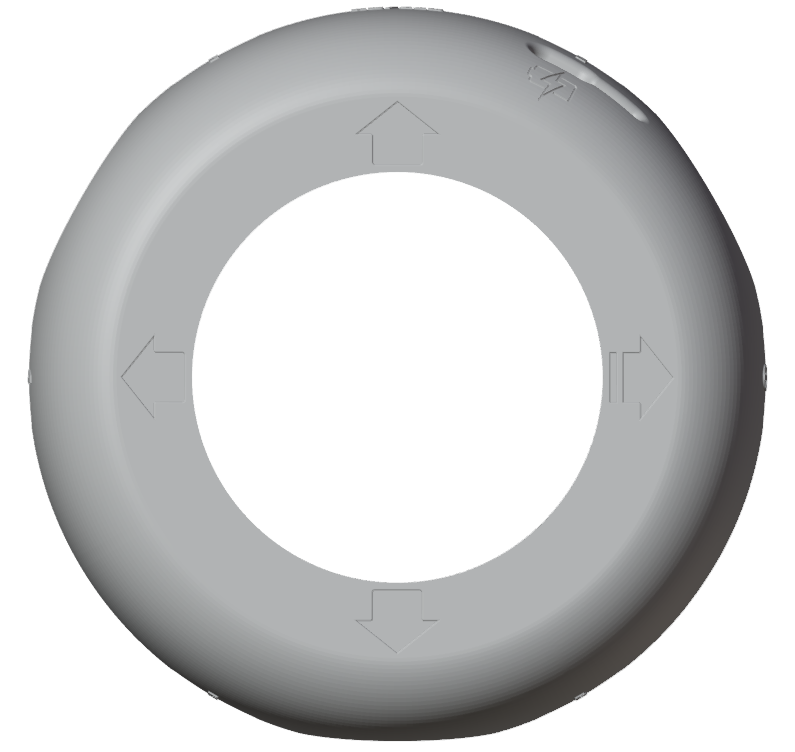
\includegraphics[width=\linewidth]{images/modelos3d/carcasa-original-superior.png}
        \caption{Vista superior}
    \end{subfigure}
    \hfill
    \begin{subfigure}{0.4\textwidth}
        \centering
        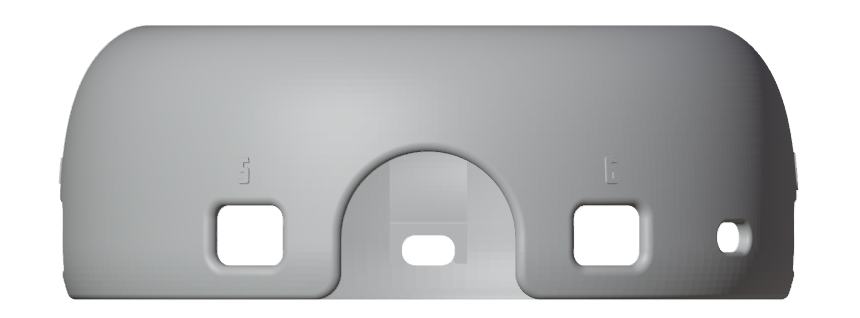
\includegraphics[width=\linewidth]{images/modelos3d/carcasa-original-frontal.png}
        \caption{Vista frontal}
    \end{subfigure}

    % -------- Segunda fila --------
    \begin{subfigure}{0.6\textwidth}
        \centering
        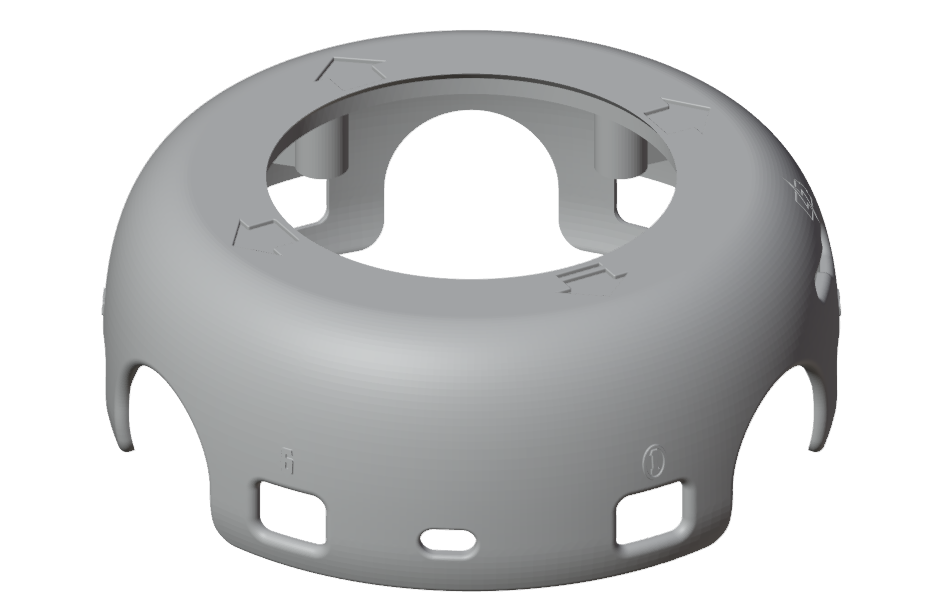
\includegraphics[width=\linewidth]{images/modelos3d/carcasa-original-3d.png}
        \caption{Vista en perspectiva}
    \end{subfigure}

    \caption{Vistas del modelo tridimensional de la carcasa original de Robotito utilizado como base para el rediseño.}
    \label{fig:carcasa-original}
\end{figure}

Además se buscaron modelos de soporte para HuskyLens, llegando a la decisión de utilizar un modelo de dos piezas (incluyendo una base y una tapa) de carcasa externa de la cámara  \cite{CarcasaHuskylens}, con dimensiones aproximadas de 5.72cm x 4.82cm x 7.3cm para la base y 5.72cm x 4.12cm x 9.6cm para la tapa.

\begin{figure}[htbp]
    \centering

    % -------- Primera fila --------
    \begin{subfigure}{0.4\textwidth}
        \centering
        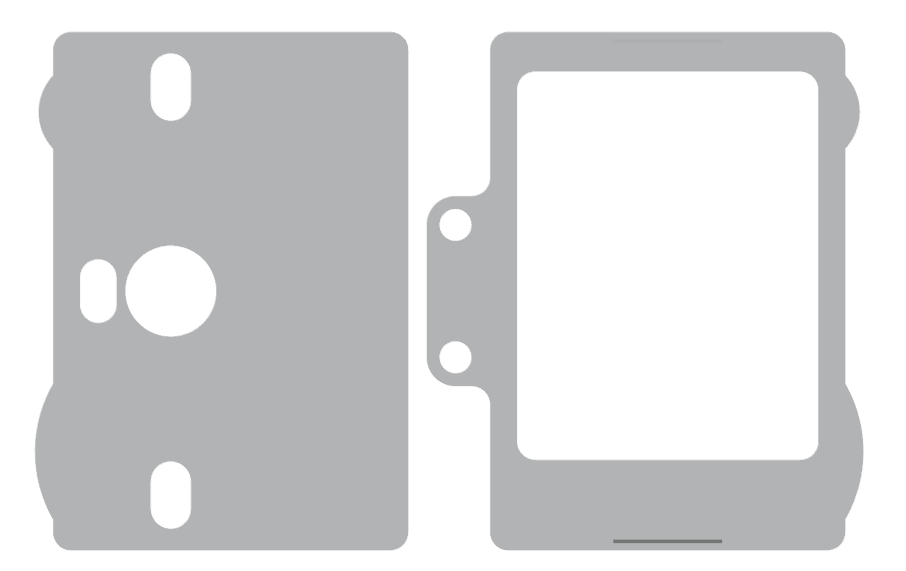
\includegraphics[width=\linewidth]{images/modelos3d/carcasa-husky-superior.png}
        \caption{Vista superior}
    \end{subfigure}
    \hfill
    \begin{subfigure}{0.4\textwidth}
        \centering
        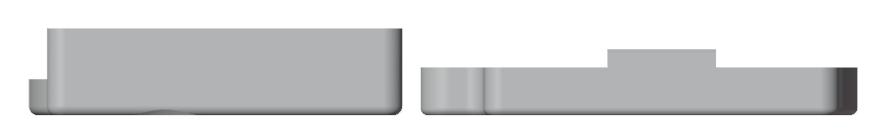
\includegraphics[width=\linewidth]{images/modelos3d/carcasa-husky-lateral.png}
        \caption{Vista Lateral}
    \end{subfigure}

    % -------- Segunda fila --------
    \begin{subfigure}{0.5\textwidth}
        \centering
        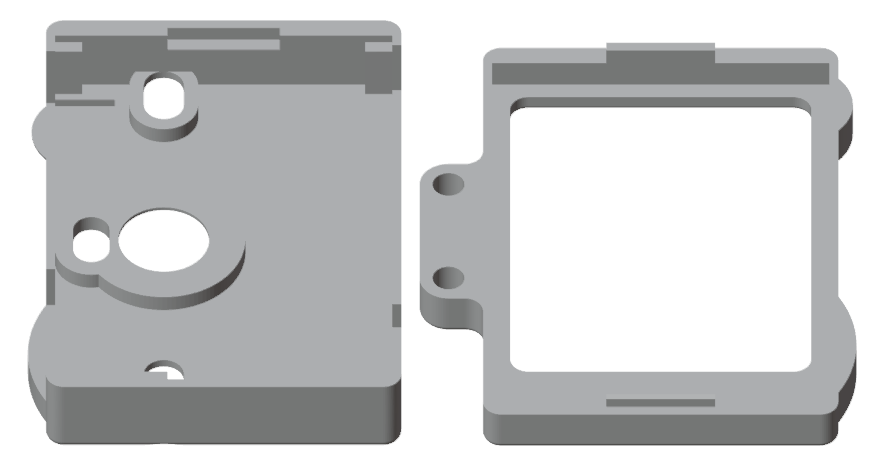
\includegraphics[width=\linewidth]{images/modelos3d/carcasa-husky-3d.png}
        \caption{Vista en perspectiva}
    \end{subfigure}

    \caption{Vistas del modelo tridimensional de la carcasa original de HuskyLens.}
    \label{fig:carcasa-husky-original}
\end{figure}

\FloatBarrier 

\subsection{Diseño conceptual}
% estructura general, criterios de decisión, integración con el robot

Con estos dos modelos como base para el diseño, se buscó fusionarlos en un solo modelo que permita agregar la cámara HuskyLens a su interior, manteniéndola fija en un ángulo determinado y de fácil acceso en caso de tener que configurarla o desarmar la estructura. Tomando como base las pruebas realizadas previas al rediseño de la carcasa, se definió el ángulo de inclinación de la cámara 16.5 grados con respecto al eje horizontal, que permite una visión cercana a Robotito, facilitando su funcionamiento, y que además logra mantener una coherencia estética y estructural con el modelo original, ya que un ángulo significativamente grande representa una pieza sobresaliente a la parte superior del robot que puede ser fácilmente rota al ser manipulada en un entorno educativo infantil.

\subsection{Proceso de modelado CAD}
% herramienta utilizada y metodología básica

La herramienta utilizada para el modelado tridimensional de la nueva carcasa fue Blender \cite{Blender} en su versión para el sistema operativo Windows. Con esta herramienta se logró importar los archivos de extensión .stl (Stereolithography) de cada modelo y trabajar sobre las superficies geométricas definidas en cada uno.

El primer paso para realizar el rediseño luego de obtenidos los dos modelos individuales de carcasa de Robotito y de cámara HuskyLens, fue ubicar a ambos en sus posiciones correspondientes al modelo objetivo. Para esto se ubica la carcasa de Robotito con el centro de su base en el origen (X=0, Y=0, Z=0) y luego se ubica el modelo de soporte de la cámara en la posición definida según las pruebas realizadas (ligeramente arriba de la parte superior de la carcasa de Robotito, sobre el borde del mismo, ubicando la zona correspondiente al lente de la cámara hacia la dirección ``frontal'' del robot, que además coincide con las ruedas frontales de Robotito, apuntando hacia ``abajo'' con una leve inclinación de 16.5 grados con respecto al plano horizontal).

Una vez ubicados ambos modelos en las posiciones correctas, se implementa una tercera estructura que respresenta la ``unión'' física entre ambos. Para eso se busca mantener la coherencia estética del modelo, intentando no utilizar ángulos muy forzados y simplificando la geometría utilizada.

Con los tres modelos presentes y ubicados en sus posiciones finales, se realizan repetidas operaciones booleanas de Unión de Blender. Esto logra unir dos piezas seleccionadas en una sola, haciendo que el modelo consista de la menor cantidad de piezas necesarias. Luego de ejecutadas las uniones se llega a un modelo de dos piezas que incluye la carcasa original de Robotito con una base para HuskyLens, y una tapa para asegurar la cámara luego de ubicada en el robot.

Finalmente, para mejorar la estética del modelo y asegurar su funcionamiento seguro como aplicación en un entorno educativo infantil, se realizaron dos agujeros (en la herramienta Blender) en el modelo de la carcasa para permitir que todo el cableado de la cámara se ubique de forma interna a la estructura del robot. Cada agujero corresponde a una entrada física de cables que permite la cámara, con sus tamaños correspondientes.

\subsection{Resultados y mejoras futuras}
% qué se logró y qué quedaría para una siguiente iteración

El resultado obtenido se detalla a continuación, donde se puede observar el diseño terminado con ambas piezas (carcasa y tapa) ya ubicados en sus respectivos lugares \\

\begin{figure}[htbp]
    \centering

    % -------- Primera fila --------
    \begin{subfigure}{0.49\textwidth}
        \centering
        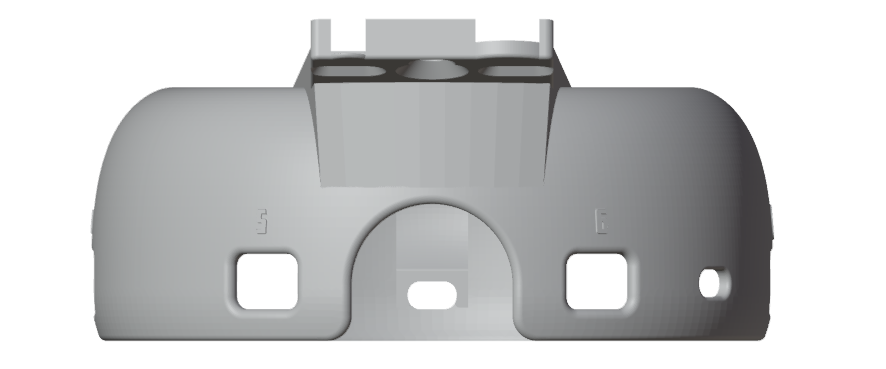
\includegraphics[width=\linewidth]{images/modelos3d/carcasa-nueva-frontal.png}
        \caption{Vista Frontal}
    \end{subfigure}
    \hfill
    \begin{subfigure}{0.49\textwidth}
        \centering
        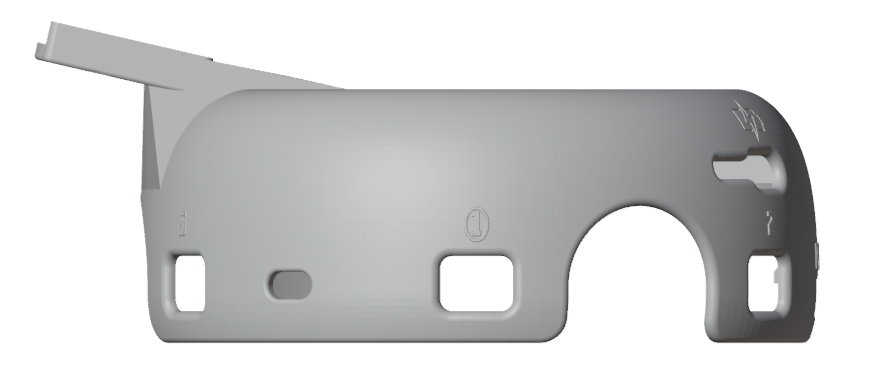
\includegraphics[width=\linewidth]{images/modelos3d/carcasa-nueva-lateral.png}
        \caption{Vista Lateral}
    \end{subfigure}

    % -------- Segunda fila --------
    \begin{subfigure}{0.49\textwidth}
        \centering
        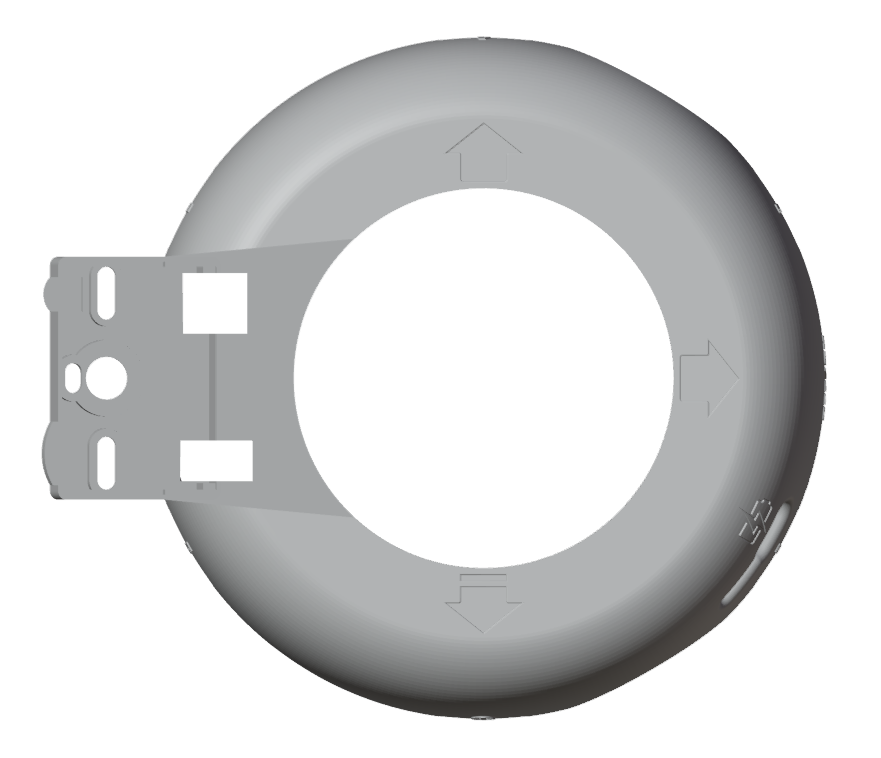
\includegraphics[width=\linewidth]{images/modelos3d/carcasa-nueva-superior.png}
        \caption{Vista Superior}
    \end{subfigure}
    \hfill
    \begin{subfigure}{0.49\textwidth}
        \centering
        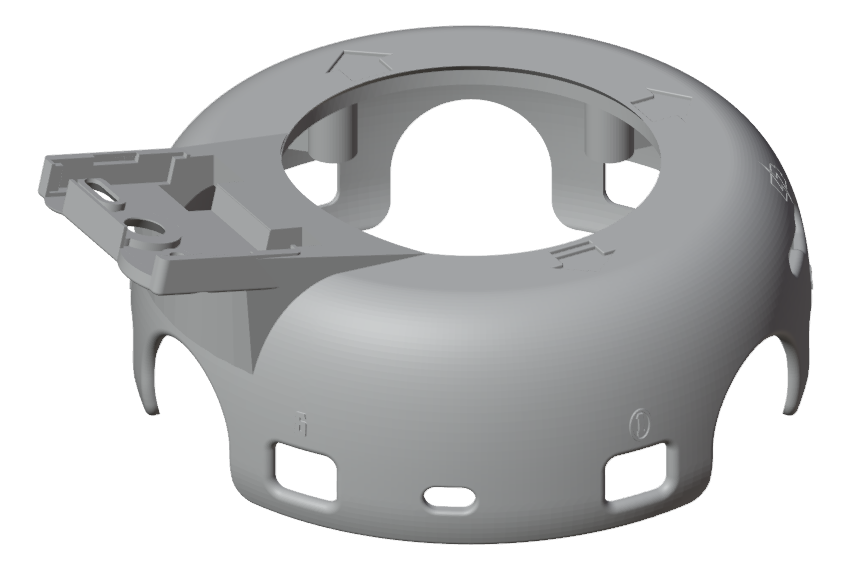
\includegraphics[width=\linewidth]{images/modelos3d/carcasa-nueva-3d.png}
        \caption{Vista en perspectiva}
    \end{subfigure}

    \caption{Vistas del modelo tridimensional de la carcasa nueva de Robotito con soporte para HuskyLens.}
    \label{fig:carcasa-husky-nueva}
\end{figure}

Infelizmente no se pudo realizar la impresión del modelo por lo que este se mantiene conceptual. Resultaría interesante un rediseño del mismo para mejorar su aspecto estético y hacerlo más llamativo a un público objetivo infantil. A partir de esto se podría analizar si genera más interés en un formato de semejanza con lo ``cotidiano'', por ejemplo animales o vehículos, o quizás un formato más ``robótico'' que despierte curiosidad por su aspecto poco común.

\end{appendix}


%%%%%%%%%%%%%%%%%%%%%%%%%%%%%%%%%%%%%%%%%%%%%%%%%%%%%%%%%%%%%%%%%%%%%%%%%%%%%%%%%%%%%%%%%%%%%%%%

\end{document}
